\def\CleanRevision{1}
\documentclass[final,5p]{elsarticle}
\ifdefined\pdfobjcompresslevel
  \pdfobjcompresslevel=0
\fi
\usepackage{amsmath,amssymb,amsfonts}
\usepackage{microtype,pifont}
\usepackage{graphicx}
\usepackage{dblfloatfix}
\usepackage[dvipsnames]{xcolor}
\usepackage{pgfplots}
\usepgfplotslibrary{groupplots}
\pgfplotsset{compat=1.18}
\usepackage{booktabs,multirow,tabularx,array,makecell}
\usepackage{algorithm,algorithmicx,algpseudocode}
\usepackage{enumitem, float,placeins}
\usepackage{caption}
\usepackage[colorlinks,bookmarksopen,bookmarksnumbered,citecolor=black, colorlinks=true,linkcolor=black,urlcolor=black,breaklinks=true]{hyperref}
\usepackage{xurl}
\usepackage{orcidlink}
\usepackage{balance}
% Permit top/bottom placement of two-column floats and reduce float starvation.
\setcounter{topnumber}{3}
\setcounter{dbltopnumber}{3}
\renewcommand{\topfraction}{0.9}
\renewcommand{\dbltopfraction}{0.9}
\renewcommand{\bottomfraction}{0.8}
\renewcommand{\textfraction}{0.05}
\renewcommand{\floatpagefraction}{0.75}
\renewcommand{\dblfloatpagefraction}{0.75}

% =========================
% Commands and styles
% =========================
\newcommand{\cmark}{\textcolor{ForestGreen}{\ding{51}}}
\newcommand{\xmark}{\textcolor{BrickRed}{\ding{55}}}
\ifdefined\CleanRevision
  \colorlet{revisiongreen}{black}
\else
  \colorlet{revisiongreen}{ForestGreen}
\fi
\newcommand{\rev}[1]{\textcolor{revisiongreen}{#1}}
\let\newrev\rev
% Use TeX primitive input for row fragments immediately before booktabs rules.
\newcommand{\TableRows}[1]{\csname @@input\endcsname{#1}}

\newcolumntype{R}[1]{>{\raggedleft\arraybackslash}m{#1}}
\newcolumntype{L}[1]{>{\raggedright\arraybackslash}m{#1}}
\newcolumntype{C}[1]{>{\centering\arraybackslash}m{#1}}

\renewcommand{\algorithmicrequire}{\textbf{Input:}}
\renewcommand{\algorithmicensure}{\textbf{Output:}}
\algrenewcommand\algorithmiccomment[1]{\hfill{\footnotesize$\triangleright$ #1}}

\makeatletter
\newcommand{\algorithmautorefname}{Algorithm}
\renewcommand{\figureautorefname}{Figure}
\renewcommand{\tableautorefname}{Table}
\renewcommand{\equationautorefname}{Eq.}
\renewcommand{\sectionautorefname}{Section}
\makeatother

\journal{Future Generation Computer Systems}

% Generated by scripts/paper/make_numbers.py.
\newcommand{\HILRequests}{12,325}
\newcommand{\SweepPeakGain}{2.51--3.68}
\newcommand{\SweepFinalGain}{2.40--3.30}
% Generated by scripts/paper/make_hil_e2e.py.
\newcommand{\HILEtoEOffered}{398}
\newcommand{\HILEtoESteered}{69}
\newcommand{\HILEtoEFullProbes}{64}
\newcommand{\HILEtoESubmitSteerPNF}{31.6}
\newcommand{\HILEtoESubmitSteerPF}{23.2}
\newcommand{\HILEtoEMigrations}{57}
\newcommand{\HILEtoEReprobeOK}{4}
\newcommand{\HILEtoEReprobeN}{4}
\newcommand{\HILLongPackets}{1,800}
\newcommand{\HILLongRecv}{1,800}
\newcommand{\HILLongRequests}{3,084}
\newcommand{\TrainingMeanMin}{57.375}
\newcommand{\TrainingMeanMax}{57.657}
\newcommand{\TrainingMeanSD}{0.156}
\begin{document}

\begin{frontmatter}

\title{AIO-Mesh: Policy-Independent Admission for Cloud-Native Orchestration over Programmable Data Planes}

\author[add1]{Hanh P. Du\orcidlink{0000-0002-8993-1164}}
\ead{hanhdp@vnu.edu.vn}

\author[add1]{Hung D. Hoang\orcidlink{0009-0004-2310-3536}}
\ead{22028293@vnu.edu.vn}

\author[add2]{Thu H. Le\orcidlink{0009-0006-4295-850X}}
\ead{lehthub1@gmail.com}

\author[add2]{Tuan X. Le\orcidlink{0009-0004-5070-9533}}
\ead{tuanlx.psa@gmail.com}

\author[add3]{Giang L. Nguyen\orcidlink{0000-0001-6184-1469}}
\ead{nlgiang@ioit.ac.vn}

\author[add1]{Hoa N. Nguyen\orcidlink{0000-0002-2565-281X}\corref{cor1}}
\ead{hoa.nguyen@vnu.edu.vn}

\cortext[cor1]{Corresponding author}

\affiliation[add1]{
organization={Department of Information Systems, VNU University of Engineering and Technology},
city={Hanoi},
postcode={11314},
country={Vietnam}
}
\affiliation[add2]{
organization={National Data Center, Ministry of Public Security},
city={Hanoi},
postcode={11309},
country={Vietnam}
}
\affiliation[add3]{
organization={Institute of Information Technology, Vietnam Academy of Science and Technology},
city={Hanoi},
postcode={11355},
country={Vietnam}
}



\begin{abstract}
\newrev{Cloud-native orchestration must reconcile policy proposals with compute capacity and programmable forwarding limits. AIO-Mesh separates replaceable proposal policies from independent admission, resource reservation, and lifecycle actuation. We evaluate this runtime with heuristic baselines and the Hardware-Aware Reinforcement Policy (HARP), which combines graph attention with placement--routing pair masking. Protected simulator policies admitted no modeled hard violations; bypassing maximum segment depth (MSD) admission exposed violations in diagnostic ablations. Policy effectiveness depended on workload and topology. Heuristics generally led in the long-lived stress benchmark, while a fixed-profile arrival-rate experiment identified conditions favoring either HARP or the Segment Routing over IPv6 (SRv6)-aware feasible heuristic (SAF-H). On a ten-switch Behavioral Model version~2 (BMv2) testbed, all \HILEtoESteered{} admitted requests reached deployment, rule readback, and steering confirmation. In-campaign probes delivered 20/20 packets for \HILEtoEFullProbes{} requests. Following a host-firewall correction, all four affected virtual network functions (VNFs) still deployed delivered 20/20 on re-probe; the fifth had been replaced. Two three-hour runs each delivered 1,800/1,800 packets to previously steered VNFs; after capacity release, 209 of 3,083 admission requests were accepted. Controlled over-depth injection confirmed drops at the expected switch. A separate 12-hour control-plane run completed \HILRequests{} requests without timeout. These results establish the measured admission-to-steering workflow and quantify the workload-dependent value and computation cost of learned selection on the evaluated simulator and software data plane.}
\end{abstract}



\begin{keyword}
\newrev{AIOps} \sep \newrev{Service function chaining} \sep \newrev{SRv6} \sep \newrev{P4} \sep \newrev{Reinforcement learning} \sep \newrev{Runtime admission}
\end{keyword}

\end{frontmatter}

\section{Introduction}
\label{sec:introduction}

Future cloud-native infrastructures are becoming distributed, programmable, and operationally dynamic. Modern service platforms combine Kubernetes clusters, edge and regional compute sites, software-defined networking, telemetry pipelines, workflow engines, and programmable forwarding devices. These infrastructures no longer host only conventional microservices; they increasingly host network and security services such as firewalls, intrusion detection systems, load balancers, deep packet inspection functions, gateways, and other virtualized or containerized network functions. Such functions are composed into service chains to enforce traffic-processing policies across tenants, applications, and security domains. As a result, infrastructure operation requires continuous decisions about where to place service functions, how to steer traffic through them, when to migrate overloaded instances, and how to preserve service objectives under changing demand, heterogeneous resources, and topology-dependent latency.

This problem is naturally an \rev{artificial intelligence for IT operations (AIOps)} problem rather than a one-shot optimization problem. In a production cloud-native environment, orchestration decisions are made from telemetry, policy intent, service demand, resource state, and runtime feedback. A learned policy must also be operated as a managed artifact: it must be loaded with the correct topology and normalization state, invoked through a stable inference path, monitored during execution, constrained by safety checks, and connected to cloud-native and network-control actuators. This view is consistent with recent \rev{machine learning operations (MLOps)} and AIOps literature, which emphasizes that machine-learning models must move from isolated training pipelines into monitored, versioned, trustworthy, and feedback-driven operational loops~\cite{kreuzberger2023mlops,diazdearcaya2024joint,eken2025mlops,bayram2025trustworthy,zhang2025aiopsllm,eramo2024architecture}. In infrastructure orchestration, however, the runtime faces an additional challenge: an AI decision may be valid in a logical model but non-deployable on the physical or programmable substrate.

Programmable data planes make this deployability gap explicit. \newrev{Segment Routing over IPv6 (SRv6) allows an ingress node to encode a list of Segment Identifiers (SIDs) in the packet header, enabling stateless traffic steering through paths and service functions~\cite{filsfils2015segment,rfc8986,rfc9352}.} \newrev{The Programming Protocol-independent Packet Processors (P4) language allows switches to expose packet-processing behavior through programmable parser, match-action, and deparser stages~\cite{jeyakumar2014p4}.} Together, SRv6 and P4 provide a practical substrate for steering cloud-native service chains without maintaining per-flow state at every intermediate node. Yet this flexibility is bounded by hardware. A programmable parser can inspect only a limited number of SIDs in a single pass. This limit, commonly represented by the Maximum Segment Depth (MSD), is not a tunable preference but a hard parsing boundary. If a selected service path requires a SID stack deeper than the supported MSD of the relevant forwarding profile, the action is not merely suboptimal; it is not admissible. \rev{Unchecked overflow may cause installation rejection, parser errors, or packet drops, depending on the forwarding target.}

Existing orchestration methods do not fully address this operational safety requirement. Classical \rev{integer linear programming (ILP)} and heuristic formulations provide useful models for service-chain placement and routing, but they \rev{may incur high solution cost or sacrifice global optimality in online operation}. Recent \rev{deep reinforcement learning (DRL)} and graph-based methods improve adaptive \rev{service function chaining (SFC)} embedding and \rev{virtual network function (VNF)} placement~\cite{wang2021drl,xiao2023twostage,liu2024sfcml,taktak2024drl,wu2025drl}, and migration-oriented studies address failure prediction, load pressure, and migration budgets~\cite{zhai2023migration,addad2022ai,qin2023sfcmigrationbudget,afrasiabi2024cluster,zhang2025sfcmigration,hu2026rlpmo}. SRv6-aware approaches such as SFCPlanner show the relevance of source-routed flow steering for service-chain planning~\cite{qiu2024sfcplanner}. \rev{Safe reinforcement learning, shielding, and invalid-action masking also provide established mechanisms for restricting unsafe actions~\cite{gu2024safe,wachi2024constraint,huang2022closer}. However, their applicability to programmable orchestration depends on whether the checked policy action corresponds to the realized forwarding configuration.} This is \rev{important} for AIOps control, where unsafe actuation can convert a policy error into a data-plane failure.

The core research question addressed in this paper is therefore: \rev{\emph{how can an AIOps runtime use learned policies for cloud-native distributed service orchestration while independently checking hardware deployability before actuation?}} This question has three coupled challenges. First, \newrev{placement, routing, SID depth, and latency depend on the substrate, and the policy must receive enough state to represent these dependencies.} Second, the runtime must distinguish hard deployability constraints from soft operational objectives. \newrev{Central processing unit (CPU), memory, and MSD feasibility} must be enforced before actuation, whereas latency, service-level pressure, and \rev{action-switching cost} can be optimized through the reward function. Third, the learned policy must be embedded into a closed-loop AIOps runtime that connects telemetry, state construction, inference, safety validation, cloud-native lifecycle management, programmable steering, and feedback monitoring.

To address these challenges, we propose \textbf{AIO-Mesh}, a hardware-safe AIOps orchestration framework for cloud-native distributed services over programmable infrastructures. AIO-Mesh treats the learned policy as one component of an operational control loop rather than as a standalone optimizer. Its runtime integrates telemetry-driven state construction, policy inference, hard-feasibility validation, smart admission control, Kubernetes/Tekton-based VNF lifecycle actions, SRv6/P4 steering, and data-plane feedback. \newrev{Within AIO-Mesh, HARP is a graph-reinforcement policy for topology-aware placement--routing selection}. HARP combines graph-attention topology encoding, \rev{masked Proximal Policy Optimization (PPO)}, invalid action masking, adaptive penalties for soft service objectives, and explicit \texttt{NO\_SAFE\_ACTION} handling under saturation. \rev{Its proposals pass through a policy-independent runtime admission boundary; migration is managed by the lifecycle workflow.}

\newrev{The distinctive contribution is an admission-to-actuation contract for programmable service infrastructure. HARP instantiates the proposal interface with established graph attention and masked policy optimization; safety enforcement belongs to the common runtime. We make three contributions:}
\begin{itemize}
\item \newrev{We specify and implement a policy-independent boundary that checks modeled compute and SRv6 depth before reservation, then associates an admitted single-VNF realization with deployment, controller confirmation, rule readback, and packet observation.}
\item \newrev{We compare HARP with Greedy, Decoupled AI (DAI), an SRv6-aware feasible heuristic (SAF-H), and a constrained shortest-path first (CSPF) pair baseline under common admission. Corrected checkpoints, matched offered traces, per-seed comparisons, ablations, and timing expose both workload-dependent acceptance and policy cost.}
\item \newrev{We validate the runtime on MicroK8s, Tekton, Mininet, and BMv2: request-correlated single-VNF actuation, controlled over-MSD fault injection, make-before-break ordering, a 12-hour control-plane run, and two three-hour occupancy conditions. The data-plane experiment checks the concrete forwarding path without attributing the runtime safety result to HARP alone.}
\end{itemize}

\section{Background and Related Work}
\label{sec:related}

This section positions AIO-Mesh at the intersection of AIOps, cloud-native resource orchestration, service function chaining, programmable data planes, and safe reinforcement learning. \newrev{AIO-Mesh addresses the runtime interface between candidate selection, local admission, and lifecycle actuation. Its implementation and evaluation distinguish these responsibilities and the evidence required to connect them.}

\subsection{AIOps and MLOps for Cloud-Native Infrastructure}
\label{subsec:related_aiops}

AIOps applies AI techniques to the operation of complex software and infrastructure systems. Typical tasks include anomaly detection, failure prediction, incident triage, capacity planning, root-cause analysis, and automated remediation. Recent AIOps and MLOps surveys emphasize that modern operational systems rely on heterogeneous telemetry and increasingly require closed-loop workflows rather than isolated predictive models~\cite{diazdearcaya2024joint,zhang2025aiopsllm}. MLOps complements this view by addressing the lifecycle of machine-learning artifacts, including model packaging, versioning, deployment, inference serving, monitoring, robustness, and rollback~\cite{kreuzberger2023mlops,eken2025mlops,bayram2025trustworthy}.

For cloud-native infrastructures, this operational perspective is essential. Placement, migration, scaling, and steering decisions are not made once; they are continuously revised as traffic demand, resource pressure, and service objectives change. Recent work on intelligent DevOps automation, Kubernetes-oriented microservice placement, elastic container management, dynamic cloud resource allocation, and computing-continuum resource selection similarly argues that automation systems must connect models, runtime evidence, and deployment actions~\cite{eramo2024architecture,ding2023kubernetes,mao2023flowcon,chen2023workloadwindows,chen2024crossedge,sedghani2024space4aid}. AIO-Mesh follows this direction but focuses on a harder class of actuation: the policy output directly affects VNF lifecycle, traffic steering, and programmable data-plane behavior. Therefore, the runtime must be fail-closed and safety-aware, not merely prediction-driven.

\begin{table*}[t]
\centering
\caption{Positioning of AIO-Mesh against representative related work. \rev{The MSD column concerns explicit SRv6 admission, not general resource-constraint handling.}}
\label{tab:related_comparison}
\renewcommand{\arraystretch}{1.15}
\resizebox{\textwidth}{!}{
\begin{tabular}{p{4.0cm}p{3.1cm}p{2.0cm}p{2.0cm}p{2.0cm}p{1.8cm}p{1.8cm}}
\toprule
\textbf{Work line} & \textbf{Primary focus} & \textbf{Cloud-native lifecycle} & \textbf{Graph-aware policy} & \rev{\textbf{SRv6 MSD admission}} & \textbf{Program- mable actuation} & \textbf{AIOps runtime} \\
\midrule
Classical ILP / greedy heuristics & SFC placement and routing & No & Limited & \rev{Varies} & No & No \\
DRL-based SFC placement~\cite{wang2021drl,taktak2024drl,li2023qosaware} & Online SFC embedding & No & Partial & No & No & No \\
\rev{Graph-assisted embedding}~\cite{xiao2023twostage,pei2025graph,liu2024sfcml} & Topology-aware embedding & No & Yes & No & No & No \\
SFC migration studies~\cite{zhai2023migration,addad2022ai,qin2023sfcmigrationbudget,afrasiabi2024cluster,zhang2025sfcmigration,hu2026rlpmo} & Load/failure migration & Partial & Varies & No & No & Limited \\
SRv6/P4 service-chain systems~\cite{stockmayer2020p4sfc,xiang2019p4sc,yan2024srv6int,li2024stsfc,ma2024sfcache} & Programmable steering & Limited & Partial & Partial & Yes & Limited \\
\newrev{Safe RL for network slicing~\cite{liu2021safeslicing,nagib2025safeslice}} & \newrev{Resource and latency constraints} & Partial & Varies & No & No & Limited \\
SFCPlanner~\cite{qiu2024sfcplanner} & SRv6-aware planning & No & Partial & Partial & Yes & No \\
AIOps/MLOps automation~\cite{kreuzberger2023mlops,diazdearcaya2024joint,eken2025mlops,bayram2025trustworthy,zhang2025aiopsllm,eramo2024architecture} & Operational ML loops & Partial & Not network-specific & No & No & Yes \\
\textbf{AIO-Mesh / HARP} & Hardware-safe AIOps orchestration & \textbf{Yes} & \textbf{Yes} & \rev{Pair-level} & \textbf{Yes} & \textbf{Yes} \\
\bottomrule
\end{tabular}
}
\end{table*}

\subsection{Learning-Based Resource and Service-Chain Orchestration}
\label{subsec:related_learning}

\rev{SFC} steers traffic through an ordered sequence of network functions, such as firewalls, intrusion detection systems, deep packet inspection functions, load balancers, and gateways~\cite{rfc7665}. In \rev{network function virtualization (NFV)}-enabled and cloud-native infrastructures, these functions are implemented as VNFs or containerized network functions that can be instantiated, scaled, migrated, and removed by software controllers. The associated orchestration problem couples placement, routing, admission, and migration: a placement decision consumes compute and memory resources, a routing decision determines latency and path depth, and a migration decision changes both the service path and the residual resource distribution. This line of work is complementary to AIO-Mesh: while prior VNF-embedding studies optimize logical resource allocation, AIO-Mesh focuses on embedding such decisions into a hardware-safe AIOps runtime with explicit programmable-data-plane admission semantics.

Classical ILP and heuristic formulations expose the structure of SFC constraints but are often unsuitable for online operation under dynamic traffic. Learning-based methods have therefore become increasingly common. DRL-SFCP formulates adaptive SFC placement as a reinforcement-learning problem~\cite{wang2021drl}; \rev{Graph convolutional network (GCN)}-based and graph-assisted approaches exploit topology information for SFC embedding and virtualized network embedding \rev{(VNE)}~\cite{xiao2023twostage,pei2025graph,liu2024sfcml}; \rev{quality-of-service (QoS)}-aware and reliable deployment methods address service-level objectives and robustness~\cite{taktak2024drl,li2023qosaware,qu2021reliable}; and recent work considers fast joint mapping for SFC deployment~\cite{wu2025drl}. Migration-oriented studies further address failure prediction, AI-assisted \newrev{fifth-generation (5G) and beyond-5G (B5G)} migration, long-term migration budgets, cluster migration, and reinforcement-learning-based migration planning~\cite{zhai2023migration,addad2022ai,qin2023sfcmigrationbudget,afrasiabi2024cluster,zhang2025sfcmigration,hu2026rlpmo}.

These methods improve adaptivity, but \rev{the cited studies primarily evaluate logical resource feasibility, latency, service reliability, or migration cost. Explicit validation of realized SRv6 SID lists against forwarding-profile MSD receives less attention.} This abstraction is problematic for AIOps orchestration because the policy is not producing recommendations; it is producing infrastructure actions.

\subsection{Programmable Data Planes and Hardware-Constrained Actuation}
\label{subsec:related_pdp}

SRv6 enables source-routed forwarding by encoding a list of SIDs in the IPv6 \newrev{Segment Routing Header (SRH)}~\cite{filsfils2015segment,rfc8986,rfc9352}. Each SID can represent a topological segment, a local behavior, or a service-processing instruction, which makes SRv6 attractive for service-chain steering without per-flow state in every intermediate device. P4 complements this model by making parser, match-action, and deparser behavior programmable~\cite{jeyakumar2014p4}. Prior work has demonstrated P4-based service chaining, SRv6 processing, runtime programmability, test generation, in-switch caching, and stateful service-function deployment~\cite{stockmayer2020p4sfc,xiang2019p4sc,yang2024p4runpro,ruffy2023p4testgen,zhao2023p4lru,ma2024sfcache,li2024stsfc}.

Programmable infrastructures, however, expose hard actuation constraints. A P4 pipeline is constrained by parser states, header stacks, match-action resources, recirculation behavior, and target-specific limits. For SRv6 service chaining, a visible constraint is \rev{MSD}, i.e., the maximum SID depth that the forwarding profile can parse or process. A route that is reachable and low-latency at the graph level can still be non-deployable if the resulting SID stack exceeds MSD. \rev{This is a per-realization forwarding constraint rather than a resource consumed cumulatively across independent flows. Its operational consequences depend on the forwarding target. IS-IS and BGP-LS advertise different SRv6 MSD types for endpoint processing and headend encapsulation~\cite{rfc9352,rfc9514}. Compressed segment lists can reduce the number of header entries when the path supports the required SID behaviors~\cite{rfc9800}.} SRv6-aware planning methods such as SFCPlanner and SRv6 adjustment based on \newrev{in-band network telemetry (INT)} show the importance of source-routed steering and telemetry-assisted reconfiguration~\cite{qiu2024sfcplanner,yan2024srv6int}.

\subsection{Safe and Graph-Aware Reinforcement Learning for Infrastructure Control}
\label{subsec:related_safe_rl}

Reinforcement learning is attractive for infrastructure orchestration because each accepted request changes the residual capacity and future feasible action set. PPO is widely used because it balances training stability and policy improvement~\cite{schulman2017proximal}. \newrev{HARP uses graph attention to aggregate node features over substrate adjacency~\cite{velickovic2018graph}. The ablation evaluates whether this aggregation helps on the complete latency-derived graphs used here.}

\newrev{SafeSlicing maps policy outputs to allocations that respect aggregate capacity~\cite{liu2021safeslicing}. SafeSlice uses a learned cost model to project allocations toward latency-feasible actions~\cite{nagib2025safeslice}. AIO-Mesh instead checks a selected placement and routing proposal against a separate admission predicate that includes segment-list depth, and applies that same predicate to heuristic and learned proposals.}

The main safety issue is constraint semantics. Reward penalties are appropriate for soft operational objectives, such as latency, \rev{service-level agreement (SLA)} pressure, load balance, and migration overhead. They are not sufficient for constraints that define binary deployability. Safe reinforcement learning and constrained policy optimization recognize the need to separate reward optimization from safety enforcement~\cite{gu2024safe,ma2022conservative,wachi2024constraint}. Invalid action masking provides a practical mechanism for discrete or structured action spaces by removing invalid actions before sampling~\cite{huang2022closer}. \newrev{Graph attention and invalid-action masking are established techniques, not algorithmic novelties of this work.} The distinctive issue addressed here is the integration of independent admission with cloud-native lifecycle control and SRv6/P4 actuation, subject to the accuracy of the checked constraints.

\subsection{Research Gap Summary}
\label{subsec:related_gap}
\sloppy
The literature shows substantial progress in cloud-native resource management, SFC placement, learning-based orchestration, programmable data-plane steering, and AIOps/MLOps automation. However, these streams remain only partially connected. \rev{Existing studies provide complementary solutions for topology-aware optimization, safe policy learning, programmable forwarding, and operational automation, but offer limited integration of these capabilities into a unified closed-loop orchestration runtime. In particular, logical placement feasibility does not necessarily establish the deployability of the resulting SRv6/P4 forwarding configuration, and policy-side feasibility checks alone may not protect against inconsistencies introduced during action realization or actuation.}

\autoref{tab:related_comparison} summarizes the positioning of AIO-Mesh. \rev{Its contribution is the integration of policy-independent admission with cloud-native lifecycle control and SRv6/P4 actuation. HARP is a replaceable policy combining established graph attention, PPO, and action masking.}

Based on this gap, AIO-Mesh is designed around four principles. \newrev{First, orchestration must account for the substrate when it checks placements and routes.} Second, hard deployability constraints must be enforced before actuation; MSD violations cannot be delegated to a soft penalty. Third, unsafe saturation should result in explicit admission rejection, not in best-effort deployment. Fourth, the learned policy must be embedded in an AIOps runtime that connects telemetry, inference, safety validation, lifecycle management, programmable steering, and feedback. These principles motivate the system model and design requirements defined in the next section.

\section{System Model and Design Requirements}
\label{sec:system_model}

This section defines the substrate, service-chain, and hardware-safety models used by AIO-Mesh. The purpose is to separate two notions that are often conflated in learning-based orchestration: an action may be attractive under an optimization objective, but still be non-deployable on the cloud-native and programmable-data-plane substrate. We therefore model the infrastructure state, the service-chain decision, the SRv6/P4 deployability constraints, and the admission semantics that the AIOps runtime must enforce before actuation.

\subsection{Cloud-Native Programmable Substrate}
\label{subsec:infrastructure_model}

We model the infrastructure as a distributed substrate graph $\mathcal{G}=(\mathcal{V},\mathcal{E})$, where each node \(v\in\mathcal{V}\) represents a cloud, edge, or regional \rev{NFV infrastructure (NFVI)} site capable of hosting virtualized or containerized network functions, and each edge \(e=(u,v)\in\mathcal{E}\) represents a physical or logical inter-site link. Each node has compute and \newrev{random-access memory (RAM)} capacities $\mathbf{c}_v=\left[c_v^{cpu},c_v^{mem}\right]$, and is associated with a programmable-data-plane profile whose SRv6 \rev{MSD} is denoted by \(m_v^{msd}\). The MSD is not a consumable resource. It is a parser-depth bound that constrains whether a candidate SID stack can be processed by the corresponding SRv6/P4 forwarding profile. Each edge \(e=(u,v)\) has a latency \(l_{uv}\). Additional link-level attributes, such as bandwidth or loss, may be enforced by the controller, but are not included in the core policy interface in order to keep the deployed observation contract stable.

At decision epoch \(t\), the residual compute state of node \(v\) is $\mathbf{r}_v(t)=\left[r_v^{cpu}(t),r_v^{mem}(t)\right]$. AIO-Mesh observes the substrate through telemetry and converts it into a policy-facing state. For a substrate with \(N=|\mathcal{V}|\) nodes, the HARP state is $s_t=(\mathbf{X}_t,\mathbf{g}_t,\mathcal{A}_{topo})$, where \(\mathbf{X}_t\in\mathbb{R}^{N\times 6}\) is the node-feature matrix, \(\mathbf{g}_t\in\mathbb{R}^{13}\) contains global request and operational features, and \(\mathcal{A}_{topo}\) is the substrate adjacency matrix. The node features encode resource pressure, MSD-related headroom or warning indicators, alert state, and topology-related context. This representation keeps the inference interface fixed while allowing the graph encoder to exploit the physical substrate topology.

\subsection{Service-Chain Request and Orchestration Decision}
\label{subsec:sfc_model}

An incoming service-chain request is represented as
\begin{equation}
q=(o_q,z_q,\mathcal{F}_q,\mathbf{d}_q,\tau_q,\kappa_q),
\end{equation}
where \(o_q\) and \(z_q\) are the traffic origin and destination, \(\mathcal{F}_q=[f_1,f_2,\ldots,f_m]\) is the ordered service-function chain, \(\mathbf{d}_q\) denotes the per-function resource demand, \(\tau_q\) is the service-level latency target, and \(\kappa_q\) is the service class or priority. For each function \(f_i\), the compute and memory demands are denoted by \(d_{q,i}^{cpu}\) and \(d_{q,i}^{mem}\).

A placement decision maps service functions to substrate nodes: $\phi_q:\mathcal{F}_q\rightarrow\mathcal{V}$, where \(\phi_q(f_i)=v\) means that \(f_i\) is instantiated or reused at node \(v\). Given a placement, the routing decision selects substrate paths between the origin, consecutive service-function locations, and the destination. The resulting end-to-end service path is
\begin{equation}
\rev{P_q=P_{o_q,\phi_q(f_1)}\oplus P_{\phi_q(f_1),\phi_q(f_2)}\oplus\cdots\oplus P_{\phi_q(f_m),z_q}.}
\label{eq:full_chain_path}
\end{equation}
\newrev{The system-level action couples placement, routing, and operational mode: $a_t=(\phi_q,P_q,m_t)$, where \(m_t\) denotes admission, reuse, scaling, or migration. HARP represents a policy decision as a compact placement--routing pair \(a_t^H=(v_t^{place},v_t^{route})\). The simulator benchmarks evaluate this compact pair for policy selection and pair-level admission. The testbed measurements reported here concern control-plane requests and baseline Kubernetes readiness; they do not establish ordered multi-VNF forwarding.}

Migration is modeled as a controlled transition from an old placement \(\phi_q^{old}\) to a new placement \(\phi_q^{new}\). Its operational cost is
\begin{equation}
C_{mig}(q,t)=\sum_{f_i\in\mathcal{F}_q}\mathbb{I}\!\left[\phi_q^{old}(f_i)\neq\phi_q^{new}(f_i)\right]\mu_i,
\end{equation}
where \(\mu_i\) summarizes deployment delay, state-transfer cost when applicable, and steering-update overhead. AIO-Mesh executes migration using a \rev{make-before-break (MBB)} discipline: the replacement function is created and verified before traffic is steered to the new path, and the old instance is removed only after steering confirmation. \rev{Migration is managed by the lifecycle workflow rather than selected as a separate HARP action.}

\subsection{Hardware-Safety and Admission Constraints}
\label{subsec:hardware_constraint_model}

For a candidate action \(a_t\), the SRv6/P4 controller translates the selected service path into a SID list
\begin{equation}
\mathcal{S}_q(a_t)=[SID_1,SID_2,\ldots,SID_{h_q(a_t)}],
\end{equation}
where \(h_q(a_t)=|\mathcal{S}_q(a_t)|\) is the induced SID-stack depth. The action is data-plane deployable only if the resulting stack can be parsed by all relevant ingress or forwarding profiles:
\begin{equation}
\rev{h_{q,v}(a_t)\le m_v^{msd},\quad\forall v\in\mathcal{P}^{parse}_q(a_t),}
\label{eq:msd_constraint}
\end{equation}
where \(\mathcal{P}^{parse}_q(a_t)\) denotes the set of nodes or profiles that must parse the SID stack \rev{and \(h_{q,v}(a_t)\) is the depth processed at profile \(v\), equal to \(h_q(a_t)\) when the original list is processed unchanged}. Equation~\eqref{eq:msd_constraint} is a hard deployability constraint. It is not a latency penalty or a degraded-service condition: if the stack exceeds the supported parser depth, the action must not be admitted.

The system-level compute and memory feasibility requirements are:
\begin{align}
\rev{\sum_{k\in\mathcal{I}_t(v)}d_k^{cpu}}&\rev{\le c_v^{cpu},\quad\forall v\in\mathcal{V},}\label{eq:cpu_constraint}\\
\rev{\sum_{k\in\mathcal{I}_t(v)}d_k^{mem}}&\rev{\le c_v^{mem},\quad\forall v\in\mathcal{V}.}\label{eq:mem_constraint}
\end{align}
\rev{Here, \(\mathcal{I}_t(v)\) denotes distinct allocated VNF instances, including temporary replacement instances during migration. Reused instances are counted once, together with any additional allocated capacity.} Constraints~\eqref{eq:msd_constraint}--\eqref{eq:mem_constraint} define target system-level feasibility conditions. The evaluated simulator policy applies pair-level checks. The 12-hour control-plane run does not exercise packet forwarding. Separate end-to-end campaigns verify the admitted path and delivery to one selected VNF; ordered traversal through multiple VNFs is outside the measured action interface.

This separation gives each candidate action one of three operational outcomes. An action is \textit{admissible} if it satisfies \rev{the implemented} compute, memory, and MSD \rev{checks} and can be passed to cloud-native and data-plane actuators. It is an \textit{unsafe candidate} if it is generated or considered internally but rejected before admission because at least one hard constraint fails. It is an \textit{admitted violation} if it is accepted by the orchestrator and later produces a data-plane violation, such as an MSD drop. A hardware-safe orchestrator may observe unsafe candidates under saturation, but it should prevent them from becoming admitted violations.

\rev{The scope of hardware safety enforced by AIO-Mesh is bounded by pair-level pre-actuation admission checks operating on controller-visible state. Let $\mathrm{Feasible}_{checked}(a_t^H,s_t)\in\{0,1\}$ denote the admission predicate evaluating modeled CPU allocatable capacity~\eqref{eq:cpu_constraint}, memory allocatable capacity~\eqref{eq:mem_constraint}, and pair-level SRv6 MSD bounds~\eqref{eq:msd_constraint} on observed telemetry state $s_t$. The runtime guarantees a fail-closed safety boundary: any proposal $a_t^H$ evaluating to $\mathrm{Feasible}_{checked}=0$ is rejected pre-actuation with a \texttt{NO\_SAFE\_ACTION} state, preventing unsafe execution.}

\rev{To relate pair-level admission to full-chain deployability, let $\mathbf{C}_{hard}(\mathcal{R},s_t)=[C_{cpu},C_{mem},C_{msd}]$ collect hard-constraint violations across all nodes and switches in the full path. The realization $\mathcal{R}(q,a_t^H,\xi_t,\Pi)$ maps request $q$ and pair $a_t^H$ to infrastructure operations given deployment context $\xi_t$ and forwarding profiles $\Pi$. The full-chain realization soundness condition is:}
\begin{equation}
    \rev{\mathrm{Feasible}_{checked}(a_t^H,s_t)=1\Longrightarrow\mathbf{C}_{hard}\!\left(\mathcal{R}(q,a_t^H,\xi_t,\Pi),s_t\right)=\mathbf{0},}
\label{eq:realization_soundness}
\end{equation}
\rev{Equation~\eqref{eq:realization_soundness} states the desired implication for a multi-function chain. The simulator metrics remain pair-level. On the testbed, the end-to-end campaigns test a realized path to one VNF with rule readback and packet observations; they do not establish the implication for an ordered chain of several VNFs.}

\begin{table*}[!tb]
\centering
\caption{\rev{Mapping of modeled hard constraints to operational failure semantics.}}
\label{tab:hard_constraint_failure_mapping}
\renewcommand{\arraystretch}{1.15}
\small
\begin{tabularx}{\textwidth}{p{2.6cm}p{4.0cm}X}
\toprule
\rev{\textbf{Constraint}} & \rev{\textbf{Violation condition}} & \rev{\textbf{Operational consequence before mitigation}} \\
\midrule
\rev{CPU capacity} & \rev{Requested CPU resources exceed the residual allocatable capacity} & \rev{Kubernetes may leave the requested pod Pending because sufficient allocatable CPU is unavailable; CPU throttling may additionally occur when a running container reaches its configured CPU limit.} \\
\rev{Memory capacity} & \rev{Requested memory exceeds residual allocatable capacity or an applicable runtime limit} & \rev{Scheduling may fail; exceeding a container memory limit can trigger out-of-memory termination, while node memory pressure may cause eviction.} \\
\rev{SRv6 MSD} & \rev{The required processing depth of a concrete SID list exceeds the relevant forwarding-profile capability} & \rev{The selected steering realization is not directly deployable under that profile. Depending on the target, unchecked execution may cause parser failure or packet drops; a supported alternative realization must be selected before actuation.} \\
\bottomrule
\end{tabularx}
\end{table*}

\subsection{Operational Objective}
\label{subsec:objective_metrics}

AIO-Mesh aims to admit as much useful service demand as possible while preserving hard deployability and controlling operational cost. Let \(A_q(t)\in\{0,1\}\) indicate whether request \(q\) is admitted at epoch \(t\), \(L_q(t)\) denote its service latency, \(C_{mig}(q,t)\) denote migration cost, and \(V_q^{sla}(t)\) denote normalized service-level violation. \rev{A general utility objective distinguishes new admissions, active services, and migration events:}
\begin{equation}
\rev{\begin{aligned}
\max_{\pi}\ \mathbb{E}_{\pi}\sum_t\Bigg[
&\alpha\sum_{q\in\mathcal{Q}_t^{new}}A_q(t)\\
&-\sum_{q\in\mathcal{Q}_t^{act}}\big(\beta L_q(t)+\delta V_q^{sla}(t)\big)\\
&-w_{\rm mig}\sum_{q\in\mathcal{Q}_t^{mig}}C_{mig}(q,t)
\Bigg].
\end{aligned}}
\label{eq:utility}
\end{equation}
subject to the hard feasibility constraints in Eqs.~\eqref{eq:msd_constraint}--\eqref{eq:mem_constraint}. \newrev{The sets \(\mathcal{Q}_t^{new}\), \(\mathcal{Q}_t^{act}\), and \(\mathcal{Q}_t^{mig}\) contain new requests, active services, and migrating services at epoch \(t\).} The coefficients \(\alpha\), \(\beta\), \(w_{\rm mig}\), and \(\delta\) control the relative importance of admission, latency, migration cost, and SLA pressure. Equation~\eqref{eq:utility} should be read as an operational objective rather than as an offline solver formulation: HARP learns to rank \rev{locally feasible placement--routing pairs}, while AIO-Mesh enforces \rev{its checked constraints} before actuation. \rev{The implemented HARP reward is a surrogate of this system-level objective.}

Accordingly, the evaluation distinguishes safe acceptance from unsafe candidate pressure and admitted MSD violations. Safe acceptance measures useful admitted demand under hard feasibility. Unsafe candidate rate measures how often the workload pushes the system outside the feasible region before admission. \newrev{The simulator admitted-MSD-violation rate reports the model predicate. The 12-hour control-plane run does not test forwarding; the separate end-to-end and fault-injection experiments use packet observations and BMv2 counters.} This distinction is essential for stress scenarios: rejecting an unsafe request may reduce raw acceptance, but it is the correct behavior if all remaining actions are non-deployable. \rev{An empty local candidate set does not prove that no feasible realization exists elsewhere.}

\subsection{Design Requirements}
\label{subsec:design_requirements}

The above model leads to five requirements for AIO-Mesh. \textbf{R1: pre-actuation constraint checking}. CPU, memory, and MSD feasibility must be checked before actuation; the policy must not rely on data-plane drops to discover unsafe actions. \newrev{\textbf{R2: substrate-aware decision making}. The orchestration state exposes the placement, routing, latency, and SID-depth information required by both learned and heuristic policies.} \textbf{R3: closed-loop observability}. The orchestrator must consume telemetry and expose decisions, admission rejections, steering status, and data-plane counters for subsequent control. \textbf{R4: cloud-native lifecycle integration}. Admitted decisions must be translated into concrete deployment, readiness checking, migration, and steering operations. \textbf{R5: safe rejection under saturation}. When no feasible action exists \rev{within the checked candidate set}, the correct outcome is \texttt{NO\_SAFE\_ACTION}, not best-effort deployment of an unsafe service path.

These requirements define the boundary between the learning policy and the operational runtime. HARP optimizes over topology-aware and hardware-feasible actions, while AIO-Mesh remains responsible for fail-closed admission, lifecycle actuation, programmable steering, and feedback validation.

\section{AIO-Mesh Architecture}
\label{sec:architecture}

AIO-Mesh is a closed-loop AIOps orchestration framework that connects a learned policy with cloud-native lifecycle control and programmable data-plane actuation. Its architectural principle is simple: \rev{the policy proposes placement--routing actions, whereas the runtime validates the selected proposal and manages deployment or migration before changing infrastructure state}. This separates policy optimization from operational admission and \rev{provides a common pre-actuation boundary for checking compute, memory, and local SRv6 MSD constraints}.

\newrev{Figure~\ref{fig:aio_mesh_architecture} presents the overall architecture.} AIO-Mesh consists of five tightly coupled functions: telemetry-driven state construction, policy inference, safety and admission control, cloud-native lifecycle actuation, and SRv6/P4 steering with feedback. HARP is the learned decision engine inside this loop. The surrounding runtime provides the operational \rev{checks} required to use HARP \rev{under the modeled constraints} in a programmable cloud-native environment.

\begin{figure*}[t]
    \centering
    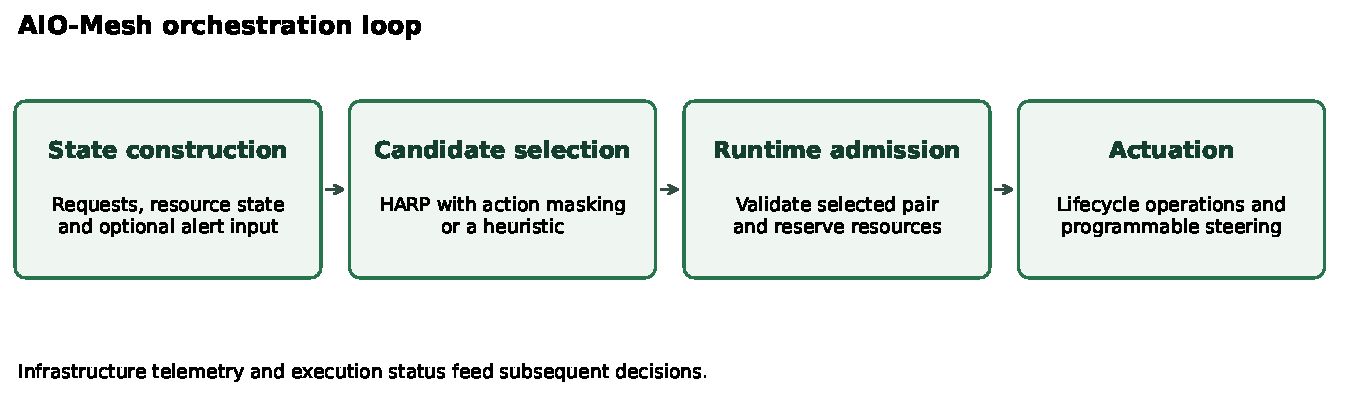
\includegraphics[width=\linewidth]{figs/overview.pdf}
    \caption{\newrev{AIO-Mesh closed-loop architecture connecting telemetry, candidate selection, local admission, cloud-native lifecycle operations, and programmable steering. HARP is a replaceable candidate-selection component. The implemented admission predicates and their relationship to forwarding realization are described in the text.}}
    \label{fig:aio_mesh_architecture}
\end{figure*}

\subsection{Closed-Loop Runtime Organization}
\label{subsec:architecture_overview}

The AIO-Mesh runtime follows an observe--decide--admit--actuate--verify loop. The telemetry layer collects resource, service, orchestration, and data-plane signals, including CPU and memory pressure, active VNF placement, service-chain demand, alert state, SRv6 steering status, and MSD-related counters. The state manager normalizes these signals and constructs the policy-facing graph state defined in \autoref{sec:system_model}. This state is passed to the policy runtime together with the substrate topology.

The policy runtime hosts two decision paths. Under stable load, AIO-Mesh may use a deterministic heuristic path to reduce overhead. Under stress \rev{or an active alert}, it invokes HARP to produce a topology-aware \rev{placement--routing proposal}. The heuristic and learned paths share the same safety boundary; neither path is allowed to actuate directly. This design makes the learned policy replaceable or retrainable without changing the admission contract of the system.

\rev{The Hybrid runtime selects between these paths using hysteresis. Let \(A_t\in\{0,1\}\) indicate an active alert and \(u_t=\max(\bar{u}^{CPU}_t,\bar{u}^{MSD}_t)\), where the terms denote mean normalized CPU utilization and the runtime's MSD accounting indicator. The decision mode is}
\begin{equation}
\rev{\mathrm{mode}_{t+1}=
\begin{cases}
\mathrm{HARP}, & u_t>0.45\ \lor\ A_t=1,\\
\mathrm{heuristic}, & u_t<0.35\ \land\ A_t=0,\\
\mathrm{mode}_t, & \text{otherwise}.
\end{cases}}
\label{eq:hybrid_gate}
\end{equation}
\rev{The MSD indicator is a policy-side accounting feature, not parser capacity consumed across flows. The gate uses the current utilization and alert input without an additional dwell-time rule. The evaluation does not compare Hybrid transitions or forecasting models.}

The admission layer is the boundary between decision making and infrastructure modification. It validates the candidate action against residual compute and memory capacity, \rev{checks the available MSD predicate for the proposed placement--routing pair}, and determines whether the action can proceed to actuation. A feasible action is admitted and passed to the actuation layer. An infeasible action is rejected before deployment or steering, and if no feasible action remains \rev{in the searched candidate set}, the runtime returns \texttt{NO\_SAFE\_ACTION}.

The actuation layer translates admitted decisions into cloud-native and network-control operations. Kubernetes and workflow automation are used to deploy, reuse, scale, or migrate VNFs. The SRv6/P4 interface generates steering state, installs the corresponding forwarding rules, and reports steering confirmation or data-plane anomalies. These post-actuation signals are fed back to the telemetry layer, closing the AIOps loop.

\subsection{Policy Runtime and State Management}
\label{subsec:policy_runtime}

AIO-Mesh treats HARP as an operational policy artifact rather than as an isolated model file. The runtime therefore manages the trained policy, topology descriptor, normalization state, safety configuration, and controller endpoints as a consistent deployment unit. This is necessary because an otherwise valid policy can become unsafe if it is executed with stale topology information, inconsistent preprocessing, or an incompatible data-plane profile.

The state manager maintains the deployed observation contract. It maps heterogeneous telemetry into a fixed graph-structured state containing node features, global request features, and the substrate adjacency matrix. The same contract is used for HARP inference and for runtime admission logging. For each decision, AIO-Mesh records the request context, selected action, feasibility outcome, rejection reason if applicable, and post-actuation feedback. These logs allow operators to distinguish policy unavailability, lack of feasible actions, controller failure, and data-plane violation.

This runtime organization follows an MLOps discipline but is specialized for network operations. Model versioning, preprocessing consistency, and observability are not sufficient by themselves; the policy also needs a fail-closed safety boundary because its output changes infrastructure state. AIO-Mesh therefore does not silently push a learned decision when the model, topology descriptor, normalization state, or controller endpoint is unavailable or inconsistent. In such cases, the runtime either falls back to a heuristic proposal path subject to the same admission checks or returns an explicit rejection.

\subsection{Safety Boundary and Admission Semantics}
\label{subsec:safety_boundary}
\label{subsec:freshness_revalidation}

\newrev{The runtime admission boundary evaluates each proposed placement--routing pair against residual CPU and memory capacity and the configured MSD predicate. Policy-side masking reduces the candidate set; admission independently checks the selected pair and reserves its local resources. A process-level lock serializes local reservations. Admission compares the decision snapshot version with the current local reservation state under that lock. The check covers local updates before reservation. External telemetry not yet ingested and changes during deployment or steering are outside that interval. If no candidate passes the configured checks, the runtime returns \texttt{NO\_SAFE\_ACTION}. The simulator benchmarks report these pair-level predicates as proposed, rejected, and admitted outcomes.}

\newrev{For requests with explicit ingress information, Section~\ref{subsec:data_plane_interface} describes the additional checks on the materialized path.}

\subsection{Cloud-Native Lifecycle Actuation}
\label{subsec:cloud_native_actuation}

\newrev{The architecture includes Kubernetes lifecycle control and a network-control interface for SRv6/P4 configuration. Section~\ref{subsec:testbed_validation} reports three complementary HIL protocols: a 12-hour control-plane run without deployment or migration, request-correlated single-VNF campaigns with Tekton and BMv2 packet probes, and two three-hour occupancy runs combining admission, readiness sampling, and probes to previously steered VNFs.}

\subsection{Programmable Data-Plane Interface}
\label{subsec:data_plane_interface}

\newrev{The forwarding interface accepts an ingress and placement and compiles an ordered sequence of switch SIDs. For the explicit-ingress path, it requires the requested depth to match the materialized list length and checks the limit of each switch profile along the path. The simulator evaluates placement--routing proposals and checks requested depth at the route anchor.}

\subsection{End-to-End Request Lifecycle}
\label{subsec:request_lifecycle}
\newrev{Algorithm~\ref{alg:aiomesh_lifecycle} summarizes the pair-selection service used by the runtime. The Hypertext Transfer Protocol (HTTP) interface accepts orchestration inputs and returns the selected pair, its bounded SID list, and the local reservation outcome.}

\begin{algorithm}[t]
\caption{Local pair-selection and reservation service}
\label{alg:aiomesh_lifecycle}
\small
\begin{algorithmic}[1]
\Require Request \(q\), local state manager, heuristic and DRL proposal providers
\Ensure Selected pair with local reservation, or rejection
\State \(mode\gets\textsc{ChooseMode}()\) using Eq.~\eqref{eq:hybrid_gate}
\If{\(mode=\mathrm{heuristic}\)}
    \State Attempt heuristic pair selection
    \State On hard-constraint failure, request a DRL/fallback proposal
\Else
    \State Request a DRL/fallback proposal
\EndIf
\State \newrev{Build the SID list using the requested depth or the compiled ingress path}
\State Check and reserve the pair under the local process lock
\If{reservation fails and the proposal was heuristic}
    \State Obtain one DRL/fallback proposal; rebuild SID list; retry reservation
\EndIf
\If{reservation fails}
    \State \Return \texttt{NO\_SAFE\_ACTION}
\EndIf
\State \Return Pair, bounded SID list, branch label and local reservation
\end{algorithmic}
\end{algorithm}

\newrev{The selected pair is returned with its local admission result. This evaluation does not establish that the pair expands into, or forwards packets through, a complete ordered VNF chain.}

\section{HARP: Hardware-Aware Reinforcement Policy}
\label{sec:harp}

HARP is the learned decision engine inside AIO-Mesh. Its objective is to select high-quality orchestration actions while preserving the hard deployability constraints defined in \autoref{sec:system_model}. The key design principle is to separate \emph{hard feasibility} from \emph{soft optimization}. CPU, memory, and SRv6 MSD feasibility are \rev{considered during policy masking and independently checked by runtime admission} before actuation. Latency, SLA pressure, load balance, and \rev{action-switching overhead} are optimized through the reward function. \rev{The policy-side mask filters locally infeasible proposals; runtime admission retains authority to reject actions before deployment.}

HARP combines three mechanisms: a graph-attention encoder for topology-aware state representation, masked policy optimization for hard constraints, and adaptive penalties for soft operational objectives. The selected action is not applied directly to the infrastructure. It is returned to the AIO-Mesh runtime, which performs final admission validation, lifecycle actuation, and SRv6/P4 steering.

\subsection{\newrev{Markov Decision Process (MDP) Formulation}}
\label{subsec:harp_mdp}

We formulate online service-chain orchestration as an \newrev{MDP}
$ \rev{\mathcal{M}=(\mathcal{S},\mathcal{A},\mathcal{P},r,\gamma),}$
where \(\mathcal{S}\) is the state space, \(\mathcal{A}\) is the action space, \(\mathcal{P}\) denotes the transition dynamics induced by traffic arrivals and infrastructure updates, \rev{\(r\)} is the reward function, and \(\gamma\) is the discount factor.

At decision epoch \(t\), the state is $ s_t=(\mathbf{X}_t,\mathbf{g}_t,\mathcal{A}_{topo}),$
where \(\mathbf{X}_t\in\mathbb{R}^{N\times 6}\) is the node-feature matrix, \(\mathbf{g}_t\in\mathbb{R}^{13}\) contains request-level and global operational features, and \(\mathcal{A}_{topo}\) is the substrate adjacency matrix. This state representation follows the system model in Section~\ref{sec:system_model}: runtime dynamics are encoded in the node and global features, while the physical topology is preserved as a graph prior.

The abstract orchestration action in Section~\ref{sec:system_model} couples placement, routing, and operational mode. \rev{In the implemented policy, HARP selects a placement--routing pair \(a_t=(v_t^{place},v_t^{route})\), encoded as}
\begin{equation}
\rev{\hat a_t=v_t^{place}N+v_t^{route},\quad \hat a_t\in\{0,\ldots,N^2-1\}.}
\label{eq:harp_action_encoding}
\end{equation}
\rev{The pair is decoded as \(v_t^{place}=\lfloor\hat a_t/N\rfloor\) and \(v_t^{route}=\hat a_t\bmod N\), giving \(|\mathcal A|=N^2\). It does not enumerate every function placement or encode a migration mode. The runtime realizes the pair using the request and deployment context. The main policy and ablation variants use a flat \(\mathrm{Discrete}(N^2)\) action head, with one logit per placement--routing pair. The same pair-level action mask is used during masked PPO training and evaluation. Earlier archived main checkpoints used factorized \(\mathrm{MultiDiscrete}([N,N])\) heads with \(2N\) logits; those legacy checkpoints are excluded from the current primary benchmark series.}

HARP does not enumerate packet-level forwarding rules. Instead, \rev{the policy evaluates local placement--routing feasibility and passes its proposal to the runtime for admission. The complete realized path and SID-list feasibility are not certified by the pair-level policy alone.}

\newrev{The evaluated main policy uses flat N²-action MaskablePPO training. Checkpoint and normalizer hashes are recorded for Vietnam, NSFNET, GEANT2, and the synthetic 25-, 50-, and 100-node substrates. Ablation uses separately trained flat-action variants under the matched-trace protocol.}

\subsection{Graph-Attention State Encoder}
\label{subsec:harp_gat}

\newrev{HARP aggregates node features over the configured adjacency using graph attention~\cite{velickovic2018graph}. An alternative multilayer perceptron (MLP) encodes the node features directly. The ablation compares the two encoders on complete latency-derived graphs.}

Let \rev{\(\mathbf{H}^{(0)}=\bar{\mathbf{X}}_t\), where \(\bar{\mathbf X}_t\) contains the normalized node features defined below.} For attention head \(k\), the unnormalized attention coefficient from node \(j\) to node \(i\) is
\begin{equation}
    e_{ij}^{(k)}
    =
    \mathrm{LeakyReLU}
    \left(
    \mathbf{a}_{k}^{\top}
    [\mathbf{W}_{k}\mathbf{h}_i \Vert \mathbf{W}_{k}\mathbf{h}_j]
    \right),
    \quad j\in\mathcal{N}(i),
\end{equation}
and the normalized attention weight is
\begin{equation}
    \alpha_{ij}^{(k)}
    =
    \frac{\exp(e_{ij}^{(k)})}
    {\sum_{r\in\mathcal{N}(i)}\exp(e_{ir}^{(k)})}.
\end{equation}
The updated node representation is
\begin{equation}
    \mathbf{h}'_i
    =
    \mathop{\Vert}_{k=1}^{K}
    \sigma
    \left(
    \sum_{j\in\mathcal{N}(i)}
    \alpha_{ij}^{(k)}\mathbf{W}_{k}\mathbf{h}_j
    \right),
\end{equation}
\newrev{Here \(K\) is the number of attention heads and \(\sigma\) is the activation. The inference architecture concatenates four 64-dimensional heads in its first attention layer and averages four heads in its second. It adds a residual projection of the node features and flattens the resulting representation in node order. Separate request and context encoders feed the same fusion network:}
\begin{equation}
\newrev{\mathbf{z}_t=\mathrm{Fuse}[\mathrm{vec}(\mathbf{H}^{(L)})\Vert\mathrm{Enc}_{req}(\bar{\mathbf g}_{t,req})\Vert\mathrm{Enc}_{ctx}(\bar{\mathbf g}_{t,ctx})].}
\end{equation}
The vector \(\mathbf{z}_t\) is passed to the actor and critic heads. \rev{Here, \(\bar{\mathbf g}_t\) denotes the normalized global features.}

\rev{The six node features comprise CPU utilization, memory utilization, an MSD accounting ratio and its complement, a CPU-alert flag, and normalized geographic context. The thirteen global features comprise three demand features, five service-type indicators, and five aggregate/context features. CPU and memory percentages are scaled by 100, MSD indicators use configured profile limits, and the assembled observation is clipped to \([0,1]\). These MSD features are policy-side proxies, not physical SID-depth validation.}

\rev{The saved normalizer subsequently applies}
\begin{equation}
\rev{\bar{x}_j=\mathrm{clip}\left(\frac{x_j-\mu_j}{\sqrt{\sigma_j^2+\epsilon_{norm}}},-c,c\right),}
\end{equation}
\rev{where \(\mu_j\) and \(\sigma_j^2\) are training-derived statistics. \rev{Inference uses the checkpoint's saved normalizer with frozen statistics.}}

\subsection{Hard-Feasibility Action Mask}
\label{subsec:harp_masking}

The central \rev{policy-side feasibility mechanism} in HARP is the hard-feasibility mask. Let \(\mathcal{F}_{loc}(s_t)\subseteq\mathcal{A}\) denote the \rev{locally feasible} action set at state \(s_t\):
\begin{equation}
\rev{\begin{aligned}
\mathcal{F}_{loc}(s_t)=\{a\in\mathcal A\mid
&C_{cpu}^{loc}(a,s_t)=0,\ C_{mem}^{loc}(a,s_t)=0,\\
&C_{msd}^{loc}(a,s_t)=0\}.
\end{aligned}}
\label{eq:feasible_set}
\end{equation}
Here \(C_{cpu}^{loc}\), \(C_{mem}^{loc}\), and \(C_{msd}^{loc}\) denote implementation-level checks, rather than a proof of the full-chain constraints. The current simulator and runtime use a flat \(N^2\) pair mask. Main retrain and ablation checkpoints have a flat \(N^2\)-logit output head. \newrev{The benchmark evaluates the flat-action main checkpoints using Stable-Baselines3~\cite{raffin2021sb3}.}

\newrev{For placement node \(p\), routing-profile node \(r\), and proposed SID-list depth \(d_q^{msd}\), runtime reservation checks the allocated CPU \(b^{cpu}_{p,t}\) and memory \(b^{mem}_{p,t}\) plus the corresponding request demand:}
\begin{equation}
\color{revisiongreen}
\begin{aligned}
M^{pair}_t(p,r)=\mathbb I[&b^{cpu}_{p,t}+d_q^{cpu}\le c_p^{cpu}\\
&\land b^{mem}_{p,t}+d_q^{mem}\le c_p^{mem}\\
&\land d_q^{msd}\le m_r^{msd}].
\end{aligned}
\label{eq:runtime_pair_mask}
\end{equation}
\newrev{Reservation increments CPU and RAM only at the placement node. The route-node MSD observation records the greatest active list depth for policy input; it is not an additive capacity consumed by concurrent flows. With an explicit ingress, path compilation additionally checks materialized SID depth against every switch profile on the compiled path. The simulator uses requested depth at the routing anchor. For distinct endpoints it also requires residual modeled link bandwidth \(B_{pr,t}\ge 10d_q^{cpu}\) Mbps. Admission reserves that bandwidth and the request expiry returns it. The local runtime reservation does not enforce the simulator bandwidth predicate.}

\newrev{The policy applies its saved normalizer and rebuilds the mask for each decision. Section~\ref{subsec:freshness_revalidation} describes the scope of the local version check.}

The actor produces a logit \(z_a\) for each action \(a\in\mathcal{A}\). HARP applies the binary mask
\begin{equation}
M_t(a)=
\begin{cases}
1, & \rev{a\in\mathcal{F}_{loc}(s_t)},\\
0, & \rev{a\notin\mathcal{F}_{loc}(s_t)},
\end{cases}
\end{equation}
and replaces infeasible logits by \(-\infty\):
\begin{equation}
\tilde{z}_a=
\begin{cases}
z_a, & M_t(a)=1,\\
-\infty, & M_t(a)=0.
\end{cases}
\end{equation}
The masked policy is then
\begin{equation}
\pi_\theta^{M}(a\mid s_t)=\frac{\exp(\tilde{z}_a)}{\sum_{b\in\mathcal{A}}\exp(\tilde{z}_b)}.
\end{equation}

\sloppy
\newrev{The flat-action main and ablation policies optimize this policy using PPO~\cite{schulman2017proximal}. At evaluation, HARP selects the highest-scoring allowed pair from the same flat N² action distribution.} With
\begin{equation}
    \rho_t(\theta)=
    \frac{\pi_\theta^{M}(a_t\mid s_t)}
    {\pi_{\theta_{old}}^{M}(a_t\mid s_t)},
\end{equation}
the clipped objective is
\begin{equation} \label{eq:ppo_clip} \mathcal{L}^{\mathrm{CLIP}}(\theta) = \mathbb{E}_t \left[ \min \left\{ \begin{aligned} &\rho_t(\theta)\hat{A}_t,\\ &\operatorname{clip}\!\left( \rho_t(\theta), 1-\epsilon_{\mathrm{PPO}}, 1+\epsilon_{\mathrm{PPO}} \right)\hat{A}_t \end{aligned} \right\} \right]. \end{equation}
with standard value and entropy terms added during training. This masking mechanism is related to invalid action masking in policy-gradient methods~\cite{huang2022closer}, \rev{but policy masking alone does not guarantee the correctness of a subsequently realized forwarding action}.

\subsection{Reward for Soft Operational Objectives}
\label{subsec:harp_penalty}

HARP uses the reward function \rev{to rank locally feasible actions and penalize operational costs}. Latency, \rev{action switching}, SLA pressure, and load balance affect service quality, but they do not by themselves determine whether an action is physically deployable. \rev{The implemented training reward is}
\begin{equation}
\rev{\begin{aligned}
r_t&=-20+\rho_{msd}I_{msd}, \quad \text{if the action is invalid};\\
r_t&=100+0.25d_q^{msd}d_q^{cpu}+30I_{core,elephant}\\
&\quad+15I_{v^{place}\ne v^{route}}-10I_{switch}-w_{svc}L_t\\
&\quad+\lambda_t\frac{L_t}{T_{svc}}I_{L_t>T_{svc}}-50I_{alert}+\rho_{msd}I_{msd}, \text{otherwise}.
\end{aligned}}
\label{eq:harp_reward}
\end{equation}
\rev{Here, \(I_{switch}\) indicates a change of placement--routing pair, \(I_{core,elephant}\) rewards a configured core node for Elephant traffic, and \(I_{msd}\) marks an MSD violation. \(I_{alert}\) marks an alert at either endpoint. The latency weights \(w_{svc}\) for IoT, Video, VoIP, Data, and Attack are 0.5, 3, 3, 0.5, and 0.05. The \(0.25d_q^{msd}d_q^{cpu}\) term rewards the product of demand and requested depth, and the 15-point term favors distinct endpoints. The configured thresholds for IoT, Video, VoIP, Data, and Attack are 10, 30, 50, 100, and 500 ms, respectively. The MSD coefficient satisfies \(\rho_{msd}\le0\), with default value \(-50\). In protected configurations, hard admission remains independent of this reward term.}

The SLA penalty multiplier is adapted from recent violation behavior:
\begin{equation}
\rev{\lambda_{k+1}=\mathrm{clip}\left(\lambda_k-\eta_\lambda(\bar{V}_k-\tau),-3000,-5\right),}
\label{eq:lambda_update}
\end{equation}
\rev{where \(\bar V_k\) is the reported violation rate averaged by the training callback, \(\tau=0.015\), \(\eta_\lambda=10\), and the initial multiplier is \(-100\). The environment uses a 20-step rolling violation indicator. The negative sign convention increases the penalty magnitude when violations exceed the target.}

This adaptive penalty regulates soft service-level pressure without weakening hard deployability constraints. \rev{The adaptive update is a reward-shaping heuristic rather than a constrained-RL safety guarantee. }

\subsection{Admission and Migration Semantics}
\label{subsec:harp_admission}
\newrev{The runtime can enumerate a local CPU-, memory-, and MSD-feasible fallback proposal when learned inference is unavailable. The selected fallback still passes independent admission. In the simulator, an empty HARP mask permits an unmasked proposal for the step, leaving the admission predicate in control of the outcome. Candidate pruning therefore includes saturated steps with empty masks.}

Migration is orchestrated by the lifecycle layer rather than emitted as a separate HARP action. The workflow creates and verifies a replacement VNF, updates steering, and removes the prior instance after the replacement path is active.

\subsection{Decision Procedure}
\label{subsec:harp_decision_procedure}
\begin{algorithm}[t]
\caption{Runtime inference path for a flat N²-action policy checkpoint}
\label{alg:harp_decision}
\small
\begin{algorithmic}[1]
\Require Request, local state, model configuration and saved normalizer
\Ensure Proposal with inference/fallback status; not a deployment outcome
\State \newrev{Load the checkpoint and normalizer with one score for each placement--routing pair}
\If{model unavailable}
    \State Return safe-search fallback or propagate hard-constraint failure
\EndIf
\State Build observation and apply the available saved normalizer
\State Build the runtime pair mask of length \(N^2\)
\State Predict a masked flat action and decode the placement--routing pair
\State On inference exception, use the guarded fallback path
\State Pass the proposal to independent local admission in Algorithm~\ref{alg:aiomesh_lifecycle}
\end{algorithmic}
\end{algorithm}

\paragraph{Computational complexity}\label{subsec:harp_complexity}
\newrev{The main and ablation actors produce \(N^2\) logits directly, and the pair mask requires \(\Theta(N^2)\) storage and processing. The graph-encoding term depends on the actual encoder, adjacency representation and attention implementation. The timing experiments in Section~\ref{subsec:decision_cost} report simulator decision costs and SAF-H scaling on synthetic grids.}

\section{Experiments and Evaluation}
\label{sec:evaluation}
\newrev{We evaluate three aspects of the orchestration design: the acceptance achieved by alternative policies under a common admission boundary; the contributions of policy representation, masking, and admission; and sensitivity to offered intensity and background occupancy. The three-workload benchmark establishes policy effectiveness under long-lived stress traffic. Ablation separates candidate selection from admission, while timing measurements quantify simulator decision cost. Load and occupancy sweeps then examine whether the policy comparison changes under different resource-pressure regimes. Table~\ref{tab:evaluation_protocols} summarizes the protocols and their measurement boundaries.}

\subsection{\newrev{Experimental Setup}}
\label{subsec:experimental_setup}
\newrev{The algorithm benchmark evaluates fixed, topology-specific main-policy checkpoints and their observation normalizers; no model is retrained during evaluation. It covers the 10-node Vietnam, 14-node NSFNET, and 23-node GEANT2 topologies under the stress load (arrival rate 1.0; request time-to-live (TTL) 100--500). The three tested workloads are Elephant stress (mapped to Heavy-tail), Burst surge (mapped to Bursty), and a separately configured Chaos workload. Each algorithm--topology--workload condition uses 20 evaluation seeds, \{42, 100, 2024, 8888, 9999, 7, 17, 73, 314, 2718, 11, 23, 47, 89, 101, 211, 512, 1024, 4096, 8192\}, and 3,000 simulator steps per seed. Algorithms share the offered-request trace within each seed; for the Bursty workload, the generator repeats the same trace across seeds.}

\newrev{The stress benchmark uses topology-specific flat \(N^2\) main checkpoints on three named substrates and three synthetic grids. All comparisons are calculated from the seed-level records.}

\newrev{The simulator reads CPU demand, memory demand, service class, and requested SID depth from the telecom trace. Uniform uses the base demands. Bursty applies deterministic peak and off-peak CPU multipliers. Heavy-tail applies a seeded CPU and SID-depth shock. Chaos uses seeded transitions between calm and stressed states, and stress changes CPU, RAM, requested depth, and service class. Request lifetime is measured in simulator steps. For the offered-intensity study, arrival probability increases to one, after which the workload scales CPU and RAM demand, requested depth, and request lifetime.}

\newrev{The Greedy baseline selects the node with the most residual CPU capacity, then the routing node with minimum latency among nodes distinct from the placement node. Decoupled AI selects the least-loaded-CPU placement and then a neighboring node with the least RAM load. SAF-H filters placement--routing pairs using CPU, memory, bandwidth, and MSD checks, then selects the pair minimizing \(0.5L+100u_{\mathrm{cpu}}+5h\), where \(L\) is measured in milliseconds, \(u_{\mathrm{cpu}}\) is a utilization fraction, and \(h\) is a hop count. The constrained shortest-path first (CSPF) baseline enumerates feasible, distinct placement--routing endpoint pairs and minimizes topology latency; hop count and residual placement CPU break ties in that order. Because the simulator action specifies only this endpoint pair and has no ingress/egress request, this is a CSPF-style pair baseline rather than a complete ingress-to-egress path computation. The paired CSPF comparison uses the protected admission mode; the other baselines also have unprotected runs, while Table~\ref{tab:simulation_acceptance_summary} reports protected results. The matched-trace ablation separately evaluates variant-specific checkpoints on Vietnam, NSFNET, and GEANT2 using 20 seeds and 3,000 simulator steps per seed--workload cell.}

\newrev{The named substrates use configured coordinates and node profiles for Vietnam, NSFNET, and GEANT2. Each node has 100 units of CPU and RAM and each modeled link starts with 10,000~Mbps. The adjacency latency thresholds are 15, 25, and 35~ms, respectively. Simulator adjacency is derived by thresholding coordinate-based pair latencies rather than importing the physical backbone edge lists. The evaluated adjacency has 45, 91, and 253 undirected edges, respectively: all three are complete graphs at these settings. Consequently, these experiments vary node count and geographic/resource profiles over complete latency-derived graphs; results should be interpreted for this graph construction.}

\begin{table*}[t]
\centering
\caption{\newrev{Protocols supporting the simulation evaluation. All use 20 evaluation seeds and 3,000 simulator steps per seed and condition. Main-policy and ablation checkpoints are distinct.}}
\label{tab:evaluation_protocols}
\color{revisiongreen}
\scriptsize
\begin{tabular}{p{0.18\textwidth}p{0.19\textwidth}p{0.25\textwidth}p{0.28\textwidth}}
\toprule
Experiment & Checkpoint/interface & Offered traffic and occupancy & Interpretation \\
\midrule
Algorithm benchmark & Corrected main retrain, flat N² head & Three stress workloads; arrival 1.0; TTL 100--500 & Six topologies; completed seed-level results with 20 evaluation seeds per cell \\
Matched-trace ablation & Variant-specific flat-action policies & Four workloads; arrival 1.0; TTL 100--500 & Candidate quality, pruning, and modeled admission; distinct trained variants \\
Timed ablation & Variant-specific flat-action policies & Ten topology--workload conditions; arrival 1.0; TTL 100--500 & Simulator normalization, inference, and stepping; external actuation excluded \\
Background chains & Corrected main flat N² checkpoints & Bursty; arrival 1.0; 0/25/50/100 persistent chains; topology-scaled TTL & Completed occupancy sweep; 20 evaluation seeds per condition \\
Arrival-rate-only & Corrected main flat N² checkpoints & Bursty; arrival probability 0.2--1.0; fixed TTL 100--500 & Isolates arrival probability; 15 topology--rate cells and 20 matched evaluation seeds per policy \\
Load-sweep protocol & Corrected main flat N² checkpoints & Bursty at seven multipliers from 0.2 to 1.5; above 1.0, scale demand, requested SID depth, and TTL & Completed combined offered-intensity sweep; 21 topology--intensity cells and 20 evaluation seeds \\
\bottomrule
\end{tabular}
\end{table*}

\newrev{The serialized timing studies used an Intel Xeon Platinum 8160 CPU at 2.10~GHz, Python 3.9.25, and NumPy 2.0.2. They measure local simulator processing.}

\subsection{\newrev{Baselines, Ablation Variants, and Metrics}}
\label{subsec:baselines_metrics}
\newrev{Decoupled AI is the benchmark name for a sequential CPU/RAM heuristic. SAF-H searches feasible placement--routing pairs using the cost defined above. The benchmark evaluates the main flat N²-action HARP checkpoints, while ablation uses separately trained flat-action variants.}

\newrev{The flat-action ablation defines Full with a graph encoder, action mask, and adaptive SLA penalty. MLP changes the encoder, NoMask removes policy masking, and NoAdapt fixes the SLA coefficient. SoftMSD uses an MSD reward penalty without a policy mask. NoMask and SoftMSD each have an evaluation mode with the MSD admission check disabled, while other resource checks stay active. Each bypass uses its corresponding checkpoint.}

\newrev{The algorithm benchmark reports safe acceptance per offered, non-skipped request and aggregates 20 seed-level rates with sample standard deviation (SD). For each protected HARP--SAF-H and HARP--CSPF contrast, paired seed-level acceptance differences are tested using the two-sided Wilcoxon signed-rank test~\cite{wilcoxon1945}; percentile-bootstrap 95\% confidence intervals (CIs) use 10,000 resamples, and Holm correction~\cite{holm1979} is applied separately across the nine topology--workload comparisons in each family. The fixed-profile arrival-rate sweep uses the same paired test, 20,000 paired percentile-bootstrap resamples, and Holm correction across its 15 topology--rate contrasts. The paired rank-biserial effect is positive when HARP tends to have higher acceptance; it describes the signed rank balance, not the magnitude in percentage points. The timing-instrumented ablation reports safe acceptance and policy-decision P95 over 20 evaluation seeds using mean and sample SD. The matched-trace ablation reports sample SD across seed--workload evaluation cells. These deviations describe evaluation variation conditional on the evaluated checkpoints, not variation across independently trained policies.}

\newrev{For the timing-instrumented and matched-trace ablations, safe acceptance is accepted requests minus the unique admitted requests violating any modeled hard CPU, memory, bandwidth, or MSD constraint, divided by offered non-skipped requests. Proposed CPU, memory, bandwidth, and MSD violation rates may overlap; the union rate is reported separately. Candidate pruning is computed over the flat $N^2$ action set.}

\newrev{All simulation rates use offered requests as the denominator unless stated otherwise. The simulator marks an arrival-free step as skipped. The stress benchmark and matched-trace ablation use arrival probability 1.0, so every seed contributes 3,000 requests. At lower intensities there can be fewer offered requests than steps. Runtime rejection and admitted violation are separate outcomes; neither is a measure of successful physical deployment. Algorithm-benchmark comparisons pair policies by topology, workload, and seed and verify identical offered-trace hashes. The matched-trace ablation likewise reuses the offered trace across variants, although policy-dependent admissions can cause simulated state trajectories to diverge.}

\subsection{\newrev{Hardware-Safe Admission under Workload Saturation}}
\newrev{All five algorithms use the same simulator admission checks in protected mode. Across nine topology--workload conditions, each policy is evaluated for 540,000 simulator steps and records zero admitted modeled hard violations. The common result demonstrates the role of admission across candidate-selection methods. Policy effectiveness is assessed separately through acceptance and the paired HARP--SAF-H differences in Table~\ref{tab:benchmark_paired_statistics} and HARP--CSPF differences in Table~\ref{tab:cspf_paired_statistics}.}



\subsection{\newrev{Simulation Results across Distributed Topologies}}
\label{subsec:simulation_results}
\newrev{Table~\ref{tab:simulation_acceptance_summary} reports mean acceptance over 20 evaluation seeds for the protected versions of five algorithms, including the CSPF-style pair baseline. Each topology--workload cell contains 20 paired seed-level trials of 3,000 simulator steps; policies share offered traces within each seed, while the Bursty generator repeats the same offered trace across seeds. Acceptance is not a full-chain safety metric.}

\begin{table*}[t]
\centering
\caption{\newrev{Protected-policy acceptance (\%; 20 seeds, mean $\pm$ sample SD). Bold marks the highest mean in each row. Profiles: E = Elephant stress, B = Burst surge, C = Chaos.}}
\label{tab:simulation_acceptance_summary}
\scriptsize
\color{revisiongreen}

\setlength{\tabcolsep}{3pt}
\resizebox{\textwidth}{!}{%
\begin{tabular}{llrrrrr}
\toprule
Network & Profile & Greedy & DAI & SAF-H & CSPF & HARP \\
\midrule
Vietnam & E & 44.07 $\pm$ 0.58 & 44.30 $\pm$ 0.61 & \textbf{44.34} $\pm$ 0.69 & 42.61 $\pm$ 0.74 & 43.00 $\pm$ 0.63 \\
Vietnam & B & 58.78 $\pm$ 0.42 & 58.78 $\pm$ 0.47 & \textbf{58.84} $\pm$ 0.63 & 56.79 $\pm$ 0.96 & 57.66 $\pm$ 0.68 \\
Vietnam & C & 45.04 $\pm$ 0.54 & 45.03 $\pm$ 0.66 & \textbf{45.08} $\pm$ 0.65 & 43.32 $\pm$ 0.65 & 43.97 $\pm$ 0.68 \\
NSFNET & E & 52.64 $\pm$ 0.55 & 52.64 $\pm$ 0.55 & \textbf{52.66} $\pm$ 0.43 & 51.45 $\pm$ 0.54 & 52.12 $\pm$ 0.66 \\
NSFNET & B & 68.27 $\pm$ 0.32 & 68.27 $\pm$ 0.32 & \textbf{68.28} $\pm$ 0.34 & 66.67 $\pm$ 0.61 & 67.41 $\pm$ 0.54 \\
NSFNET & C & 53.73 $\pm$ 0.69 & 53.73 $\pm$ 0.69 & \textbf{53.82} $\pm$ 0.66 & 52.07 $\pm$ 0.73 & 52.98 $\pm$ 0.79 \\
GEANT2 & E & 64.73 $\pm$ 0.47 & 64.71 $\pm$ 0.47 & 64.67 $\pm$ 0.40 & 64.25 $\pm$ 0.54 & \textbf{64.77} $\pm$ 0.65 \\
GEANT2 & B & 79.64 $\pm$ 0.25 & 79.64 $\pm$ 0.25 & 79.68 $\pm$ 0.26 & 80.30 $\pm$ 0.48 & \textbf{80.49} $\pm$ 0.49 \\
GEANT2 & C & 66.60 $\pm$ 0.48 & 66.60 $\pm$ 0.48 & \textbf{66.70} $\pm$ 0.50 & 65.84 $\pm$ 0.69 & 66.46 $\pm$ 0.77 \\
\bottomrule
\end{tabular}%
}
\end{table*}

\newrev{A decision-level audit of Greedy and DAI on the same 20 offered seeds per cell explains their identical protected acceptance in five cells (NSFNET E/B/C and GEANT2 B/C). The placement node matched in all 60,000 decisions in each of those cells; the complete placement--route pair matched in only 3.49--7.19\% of decisions. Both policies had identical seed-level safe acceptance in all 20 seeds of each cell. Greedy chooses maximum residual CPU and DAI chooses minimum CPU load; these criteria select the same placement in the observed trajectories. Their route rules differ, so equality of acceptance does not imply identical actions. The audit compares actions at corresponding steps on the policies' separate trajectories with matched offered traces.}

\newrev{All five protected algorithms recorded zero admitted hard violations in the nine simulator conditions. HARP exceeded SAF-H in the GEANT2 Elephant-stress and Burst-surge cells, and remained below SAF-H in the other seven cells. HARP exceeded CSPF in all nine cell means. Tables~\ref{tab:benchmark_paired_statistics} and~\ref{tab:cspf_paired_statistics} report paired seed-level comparisons against SAF-H and CSPF with Holm correction. The refreshed analysis uses the fixed N² checkpoints and 20 evaluation seeds per cell; it does not claim variation across independently trained policies. The matched-trace ablation below separately evaluates candidate masking and local admission.}

\begin{table}[t]
\color{revisiongreen}
\centering
\caption{\newrev{HARP--SAF-H acceptance differences ($\Delta$, percentage points; 20 paired seeds). Intervals: bootstrap 95\% CI; $p_H$: Wilcoxon $p$ with Holm correction across nine conditions; $r$: rank-biserial effect. Profiles E/B/C follow Table~\ref{tab:simulation_acceptance_summary}.}}
\label{tab:benchmark_paired_statistics}
\scriptsize
\setlength{\tabcolsep}{3pt}
\resizebox{\columnwidth}{!}{%
\begin{tabular}{llrrrr}
\toprule
Network & Profile & $\Delta$ & 95\% CI & $p_H$ & $r$ \\
\midrule
Vietnam & E & -1.335 & [-1.603, -1.052] & 2.29e-05 & -0.990 \\
Vietnam & B & -1.185 & [-1.340, -1.027] & 1.72e-05 & -1.000 \\
Vietnam & C & -1.108 & [-1.277, -0.945] & 1.72e-05 & -1.000 \\
NSFNET & E & -0.540 & [-0.715, -0.370] & 0.000523 & -0.989 \\
NSFNET & B & -0.868 & [-1.050, -0.683] & 1.72e-05 & -1.000 \\
NSFNET & C & -0.842 & [-1.055, -0.618] & 4.77e-05 & -0.971 \\
GEANT2 & E & 0.103 & [-0.093, 0.287] & 0.171 & 0.358 \\
GEANT2 & B & 0.808 & [0.645, 0.978] & 0.000523 & 1.000 \\
GEANT2 & C & -0.242 & [-0.460, -0.028] & 0.0537 & -0.579 \\
\bottomrule
\end{tabular}%
}
\end{table}

\newrev{The HARP--SAF-H paired comparison is conditional on the fixed N² checkpoints and simulator configuration. It estimates variation across evaluation seeds and does not quantify uncertainty across independently trained policies. Although each seed uses a shared offered trace, policy-dependent decisions can lead to different subsequent simulator states; the paired test therefore compares seed-level outcomes rather than request-level counterfactuals.}

\begin{table}[t]
\centering
\color{revisiongreen}
\caption{\newrev{Paired protected HARP--CSPF safe-acceptance differences (percentage points; 20 matched seeds). CIs are percentile-bootstrap 95\%; $p_H$ is the two-sided Wilcoxon $p$-value with Holm correction across nine conditions; $r$ is the paired rank-biserial effect.}}
\label{tab:cspf_paired_statistics}
\scriptsize
\setlength{\tabcolsep}{2.5pt}
\resizebox{\columnwidth}{!}{%
\begin{tabular}{llrrrr}
\toprule
Network & Profile & $\Delta$ & 95\% CI & $p_H$ & $r$ \\
\midrule
Vietnam & E & 0.392 & [0.215, 0.577] & 0.00142 & 0.810 \\
Vietnam & B & 0.872 & [0.603, 1.130] & 0.000187 & 0.943 \\
Vietnam & C & 0.650 & [0.477, 0.828] & 0.000787 & 1.000 \\
NSFNET & E & 0.672 & [0.487, 0.867] & 4.58e-05 & 0.981 \\
NSFNET & B & 0.742 & [0.560, 0.932] & 1.72e-05 & 1.000 \\
NSFNET & C & 0.902 & [0.655, 1.143] & 0.000787 & 0.989 \\
GEANT2 & E & 0.518 & [0.305, 0.718] & 0.00105 & 0.857 \\
GEANT2 & B & 0.183 & [0.045, 0.328] & 0.0759 & 0.462 \\
GEANT2 & C & 0.623 & [0.425, 0.832] & 0.00105 & 0.947 \\
\bottomrule
\end{tabular}%
}
\end{table}

\subsection{\newrev{Ablation Study}}
\label{subsec:ablation_study}
\newrev{Table~\ref{tab:vietnam_ablation_summary} compares seven Vietnam ablation variants under Uniform and Bursty traffic, with 20 evaluation seeds and 3,000 simulator steps per seed. It summarizes safe acceptance and the P95 policy-decision interval; the latter includes normalization, inference, and simulator stepping but excludes metric collection and external actuation.}

\begin{table}[t]
\centering
\caption{\newrev{Vietnam ablation (20 seeds; mean $\pm$ sample SD). Safe: safe acceptance; Viol.: admitted hard violations. MSD off disables MSD admission only; other resource checks remain active. The MLP variant uses a multilayer perceptron policy.}}
\label{tab:vietnam_ablation_summary}
\scriptsize
{\color{revisiongreen}
\setlength{\tabcolsep}{3pt}
\resizebox{\columnwidth}{!}{%
\begin{tabular}{lrrr}
\toprule
Variant & Safe (\%) & P95 (ms) & Viol. (\%) \\
\midrule
\multicolumn{4}{l}{\textit{Uniform}} \\
Full & 47.10 $\pm$ 0.54 & 2.201 $\pm$ 0.111 & 0.00 $\pm$ 0.00 \\
MLP & 47.36 $\pm$ 0.49 & 1.401 $\pm$ 0.066 & 0.00 $\pm$ 0.00 \\
NoMask & 10.42 $\pm$ 0.63 & 2.046 $\pm$ 0.050 & 0.00 $\pm$ 0.00 \\
NoMask (MSD off) & 10.42 $\pm$ 0.63 & 2.031 $\pm$ 0.053 & 0.00 $\pm$ 0.00 \\
SoftMSD (MSD off) & 24.02 $\pm$ 1.39 & 2.076 $\pm$ 0.076 & 0.01 $\pm$ 0.02 \\
SoftMSD (MSD on) & 23.89 $\pm$ 1.45 & 2.091 $\pm$ 0.060 & 0.00 $\pm$ 0.00 \\
NoAdapt & 47.05 $\pm$ 0.55 & 2.168 $\pm$ 0.092 & 0.00 $\pm$ 0.00 \\
\multicolumn{4}{l}{\textit{Bursty}} \\
Full & 56.83 $\pm$ 0.78 & 2.250 $\pm$ 0.062 & 0.00 $\pm$ 0.00 \\
MLP & 57.27 $\pm$ 0.61 & 1.457 $\pm$ 0.034 & 0.00 $\pm$ 0.00 \\
NoMask & 13.06 $\pm$ 0.75 & 2.128 $\pm$ 0.066 & 0.00 $\pm$ 0.00 \\
NoMask (MSD off) & 13.06 $\pm$ 0.75 & 2.117 $\pm$ 0.069 & 0.00 $\pm$ 0.00 \\
SoftMSD (MSD off) & 23.49 $\pm$ 0.74 & 2.150 $\pm$ 0.054 & 0.04 $\pm$ 0.04 \\
SoftMSD (MSD on) & 23.77 $\pm$ 1.08 & 2.150 $\pm$ 0.058 & 0.00 $\pm$ 0.00 \\
NoAdapt & 56.52 $\pm$ 0.59 & 2.254 $\pm$ 0.062 & 0.00 $\pm$ 0.00 \\
\bottomrule
\end{tabular}%
}
}
\end{table}

\newrev{With MSD admission disabled, the soft-penalty variant admits modeled hard violations under both Uniform and Bursty traffic. Enabling admission reduces the observed violation rate to zero. This diagnostic comparison illustrates why a reward penalty alone is insufficient to enforce the checked MSD constraint. Table~\ref{tab:timed_full_coverage} extends the full-policy measurements to the other evaluated substrate--workload conditions.}

\newrev{Table~\ref{tab:vietnam_ablation_summary} and Appendix Figure~\ref{fig:ablation_cost} show that graph encoding does not provide an acceptance advantage over the evaluated MLP variant in the two timing-instrumented Vietnam workloads: the full policy achieves 47.10\% and 56.83\% safe acceptance, versus 47.36\% and 57.27\% for MLP. Its mean seed-level decision P95 is also higher (2.201 and 2.250~ms versus 1.401 and 1.457~ms). These results do not establish a benefit from GAT in these conditions. Full and NoAdapt have similar mean safe acceptance in both workloads. These acceptance results do not determine whether adaptation improves service quality. The Full--NoMask difference motivates examining candidate quality, while the paired admission-on/off diagnostic addresses enforcement directly.}



\newrev{Table~\ref{tab:timed_full_coverage} summarizes full-policy acceptance and timing across ten topology--workload conditions. Each condition includes 20 seeds and records zero admitted modeled hard violations. Workload and execution conditions also affect timing, so the differences cannot be attributed to substrate size alone.}
\begin{table}[t]
\centering
\caption{\newrev{Full-policy safe acceptance and decision timing (20 seeds; mean $\pm$ sample SD). Timing summarizes seed-level P95 values; it is not a pooled request-level P95.}}
\label{tab:timed_full_coverage}
{\color{revisiongreen}\scriptsize
\setlength{\tabcolsep}{3pt}
\resizebox{\columnwidth}{!}{%
\begin{tabular}{llrr}
\toprule
Network & Workload & Safe (\%) & P95 (ms) \\
\midrule
GEANT2 & Bursty & 80.52 $\pm$ 0.46 & 2.969 $\pm$ 0.032 \\
GEANT2 & Uniform & 71.32 $\pm$ 0.36 & 2.802 $\pm$ 0.079 \\
NSFNET & Bursty & 66.83 $\pm$ 0.56 & 2.242 $\pm$ 0.051 \\
NSFNET & Chaos & 52.34 $\pm$ 0.73 & 2.223 $\pm$ 0.063 \\
NSFNET & Heavy-tail & 51.43 $\pm$ 0.54 & 2.187 $\pm$ 0.055 \\
NSFNET & Uniform & 56.81 $\pm$ 0.69 & 2.173 $\pm$ 0.025 \\
Vietnam & Bursty & 56.83 $\pm$ 0.78 & 2.250 $\pm$ 0.062 \\
Vietnam & Chaos & 43.31 $\pm$ 0.84 & 1.986 $\pm$ 0.031 \\
Vietnam & Heavy-tail & 42.79 $\pm$ 0.70 & 2.105 $\pm$ 0.145 \\
Vietnam & Uniform & 47.10 $\pm$ 0.54 & 2.201 $\pm$ 0.111 \\
\bottomrule
\end{tabular}%
}}
\end{table}

\subsection{\newrev{Matched-Trace Candidate Pruning and Admission}}
\label{subsec:mask_admission}
\newrev{We evaluated seven ablation variants on Vietnam, NSFNET, and GEANT2 using four workloads (Uniform, Bursty, Heavy-tail, and a separately configured Chaos profile), 20 evaluation seeds, and 3,000 simulator steps per seed--workload cell. Run metadata records the checkpoint and observation normalizer for each variant. For each topology, workload, and seed, all variants use the same offered-request trace. Table~\ref{tab:mask_admission} reports the mean and sample standard deviation across the 80 seed--workload cells per topology; these values describe evaluation variation rather than uncertainty across independently trained policies.}

{\color{revisiongreen}
\begin{table*}[t]
\centering
\caption{Candidate pruning and local admission outcomes under matched traces (20 evaluation seeds across four workloads; mean $\pm$ sample SD over 80 seed--workload cells per topology, percentages). Empty-mask and conditional pruning columns report means.}
\label{tab:mask_admission}
\scriptsize
\begin{tabular}{llrrrrr}
\toprule
Topology & Variant & All pruning & Empty mask & Pruning if nonempty & Admitted violations & Safe acceptance \\
\midrule
Vietnam & Full & 84.20 $\pm$ 2.76 & 52.68 & 66.61 & 0.00 $\pm$ 0.00 & 47.51 $\pm$ 5.71 \\
Vietnam & MLP & 83.61 $\pm$ 2.99 & 52.40 & 65.56 & 0.00 $\pm$ 0.00 & 47.84 $\pm$ 5.75 \\
Vietnam & NoAdapt & 84.19 $\pm$ 2.72 & 52.77 & 66.53 & 0.00 $\pm$ 0.00 & 47.44 $\pm$ 5.56 \\
Vietnam & NoMask & 0.00 $\pm$ 0.00 & 0.00 & 0.00 & 0.00 $\pm$ 0.00 & 13.26 $\pm$ 2.25 \\
Vietnam & NoMask (MSD off) & 0.00 $\pm$ 0.00 & 0.00 & 0.00 & 0.00 $\pm$ 0.01 & 13.25 $\pm$ 2.24 \\
Vietnam & SoftMSD (MSD off) & 0.00 $\pm$ 0.00 & 0.00 & 0.00 & 0.07 $\pm$ 0.08 & 24.05 $\pm$ 1.28 \\
Vietnam & SoftMSD (MSD on) & 0.00 $\pm$ 0.00 & 0.00 & 0.00 & 0.00 $\pm$ 0.00 & 24.20 $\pm$ 1.36 \\
NSFNET & Full & 80.94 $\pm$ 3.55 & 43.23 & 66.42 & 0.00 $\pm$ 0.00 & 56.85 $\pm$ 6.18 \\
NSFNET & MLP & 80.56 $\pm$ 3.33 & 42.98 & 65.91 & 0.00 $\pm$ 0.00 & 57.14 $\pm$ 6.01 \\
NSFNET & NoAdapt & 81.34 $\pm$ 3.36 & 43.47 & 66.98 & 0.00 $\pm$ 0.00 & 56.62 $\pm$ 6.11 \\
NSFNET & NoMask & 0.00 $\pm$ 0.00 & 0.00 & 0.00 & 0.00 $\pm$ 0.00 & 27.13 $\pm$ 3.43 \\
NSFNET & NoMask (MSD off) & 0.00 $\pm$ 0.00 & 0.00 & 0.00 & 0.00 $\pm$ 0.00 & 27.13 $\pm$ 3.43 \\
NSFNET & SoftMSD (MSD off) & 0.00 $\pm$ 0.00 & 0.00 & 0.00 & 0.00 $\pm$ 0.00 & 44.60 $\pm$ 6.35 \\
NSFNET & SoftMSD (MSD on) & 0.00 $\pm$ 0.00 & 0.00 & 0.00 & 0.00 $\pm$ 0.00 & 44.60 $\pm$ 6.35 \\
GEANT2 & Full & 74.72 $\pm$ 4.72 & 29.32 & 64.24 & 0.00 $\pm$ 0.00 & 70.71 $\pm$ 6.23 \\
GEANT2 & MLP & 73.95 $\pm$ 4.66 & 29.29 & 63.16 & 0.00 $\pm$ 0.00 & 70.76 $\pm$ 6.26 \\
GEANT2 & NoAdapt & 75.26 $\pm$ 4.39 & 29.48 & 64.92 & 0.00 $\pm$ 0.00 & 70.54 $\pm$ 6.25 \\
GEANT2 & NoMask & 0.00 $\pm$ 0.00 & 0.00 & 0.00 & 0.00 $\pm$ 0.00 & 34.11 $\pm$ 3.29 \\
GEANT2 & NoMask (MSD off) & 0.00 $\pm$ 0.00 & 0.00 & 0.00 & 0.00 $\pm$ 0.01 & 34.10 $\pm$ 3.29 \\
GEANT2 & SoftMSD (MSD off) & 0.00 $\pm$ 0.00 & 0.00 & 0.00 & 0.01 $\pm$ 0.02 & 26.54 $\pm$ 2.36 \\
GEANT2 & SoftMSD (MSD on) & 0.00 $\pm$ 0.00 & 0.00 & 0.00 & 0.00 $\pm$ 0.00 & 26.60 $\pm$ 2.36 \\
\bottomrule
\end{tabular}
\end{table*}
}

{\color{revisiongreen}
\begin{table}[t]
\centering
\caption{\newrev{Proposed and admitted hard violations (\%; 720,000 simulator steps per variant across topologies, workloads, and seeds). CPU/RAM/bandwidth (BW)/MSD proposal rates overlap; Union counts requests with any proposed hard violation, and Admitted reports admitted hard violations.}}
\label{tab:proposal_violations}
\scriptsize
\setlength{\tabcolsep}{3pt}
\resizebox{\columnwidth}{!}{%
\begin{tabular}{lrrrrrr}
\toprule
Variant & CPU & RAM & BW & MSD & Union & Admitted \\
\midrule
Full & 41.641 & 6.069 & 0.000 & 0.029 & 41.642 & 0.000 \\
MLP & 41.415 & 1.564 & 0.000 & 0.122 & 41.416 & 0.000 \\
NoAdapt & 41.798 & 5.685 & 0.000 & 0.000 & 41.799 & 0.000 \\
NoMask & 75.139 & 3.653 & 0.000 & 0.002 & 75.168 & 0.000 \\
NoMask (MSD off) & 75.146 & 3.633 & 0.000 & 0.001 & 75.175 & 0.001 \\
SoftMSD (MSD off) & 68.214 & 2.863 & 0.000 & 0.328 & 68.271 & 0.025 \\
SoftMSD (MSD on) & 68.136 & 2.819 & 0.000 & 0.352 & 68.198 & 0.000 \\
\bottomrule
\end{tabular}%
}
\end{table}
}

\newrev{Appendix Figure~\ref{fig:ablation_pruning} compares candidate pruning and safe acceptance. Candidate pruning is the per-step fraction of the flat $N^2$ action set removed before policy sampling. Runtime rejection and safe acceptance use offered, non-skipped requests as the denominator; admitted hard violations are the union of the modeled CPU, RAM, bandwidth, and MSD violations among admitted requests. The full policy prunes 74.72--84.20\% of candidates across the three topologies, including decision states with an empty mask. Table~\ref{tab:mask_admission} separates empty-mask frequency and conditional pruning. Empty masks remove every candidate. With equal-length runs, pruning fraction \(p\) and empty-mask fraction \(e\) give conditional pruning \((p-e)/(1-e)\). Empty-mask frequency and rejection rate are marginal summaries. They do not establish how many proposals from nonempty masks were rejected. The pooled ablation comprises 720,000 simulator steps per variant. Each step in this protocol offers one request. On this evaluation, the no-mask variant proposed a hard-invalid action on 75.17\% of offered requests, compared with 41.64\% for the full policy; the admission check rejected these proposals, and no hard-invalid requests were admitted in either protected condition. Because the policies differ as well as the masks, this comparison does not isolate the causal effect of masking. Per-constraint proposal rates in Table~\ref{tab:proposal_violations} overlap; their union avoids double-counting requests. The MSD reward coefficient is $-50$. With the same NoMask checkpoint, disabling MSD admission admitted 9 MSD-invalid actions over the 720,000-step evaluation (0.00125\%); the SoftMSD checkpoint admitted 182 such actions (0.02528\%) with MSD admission disabled and none with it enabled. CPU, RAM, and bandwidth checks remained active in both MSD-admission-bypass conditions. Although paired variants receive the same offered trace, different admission decisions can change later states, so request outcomes are not per-request counterfactual pairs. The reported latency field measures simulated service latency, not policy-computation overhead. These results characterize simulator predicates; forwarding on the BMv2 testbed is reported separately in Section~\ref{subsec:testbed_validation}.}



\subsection{\newrev{Hardware-in-the-Loop Testbed Validation}}
\label{subsec:testbed_validation}
\newrev{Figure~\ref{fig:testbed_architecture_eval} depicts the orchestration backend, policy engine, admission service, MicroK8s/Tekton lifecycle control, Mininet, Behavioral Model version~2 (BMv2) P4 switches, and SRv6 components. Three complementary HIL protocols are reported: a 12-hour API and baseline-readiness run (Table~\ref{tab:hil_12h}), request-correlated deployment and forwarding campaigns (Tables~\ref{tab:hil_e2e} and~\ref{tab:hil_msd}), and two three-hour admission/readiness/packet-probe runs at different occupancy levels (Table~\ref{tab:hil_longrun}). Ten BMv2 switches run in Mininet with the per-switch MSD limits of the Vietnam profile, and the MicroK8s cluster has four nodes; all forwarding results refer to this software data plane.}

\begin{figure*}[t]
    \centering
    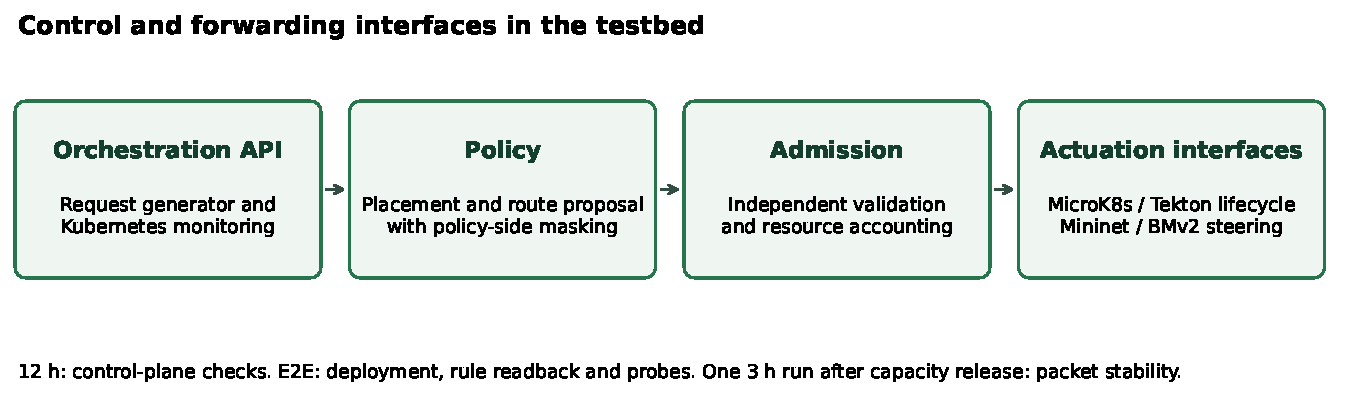
\includegraphics[width=\linewidth]{figs/testbed.pdf}
    \caption{\newrev{AIO-Mesh testbed components, including MicroK8s, Tekton, Mininet, BMv2 P4 switches, SRv6 interfaces, and runtime admission control. The diagram shows architecture; measured quantities are reported in Tables~\ref{tab:hil_12h}--\ref{tab:hil_longrun}.}}
    \label{fig:testbed_architecture_eval}
\end{figure*}

\newrev{The 12-hour experiment exercises orchestration requests through the API and samples Kubernetes readiness once per minute. Readiness is defined for the seven Deployments in the run baseline.}

\newrev{The 12-hour control-plane HIL used one sequential worker, a 3.5~s request interval, and no state reset. Table~\ref{tab:hil_12h} is regenerated from the raw request and readiness logs. Requests asked for SID depth 1 (4,964 requests) or 2 (7,361); the Vietnam profile lists per-node MSD limits of 10, 10, 5, 5, 4, 8, 4, 5, 10, and 5 SID entries. The log classified 9,672 rejections as \texttt{msd\_violation} (89.0\% of rejected requests) and 1,198 as \texttt{no\_safe\_action}, with no separate CPU/RAM-capacity category. The MSD-labeled outcomes primarily reflect a mismatch between requested depth and materialized path depth; they do not establish parser overflow. The \texttt{no\_safe\_action} label is the catchall for hard-constraint errors without a more specific classification. The log does not give the underlying error text. The workload did not request new deployments, so these counts describe admission outcomes only. All admitted requests were attributed to Hybrid:DRL; rejected requests have no policy-method attribution in the records. Client-observed API round-trip time (RTT) was 118.19/169.95/229.40~ms at P50/P95/P99. Among admitted requests, backend inference P50/P95/P99 was 74.89/117.73/154.42~ms and admission validation was 18.28/29.47/41.53~ms; these component percentiles are computed separately and must not be added to obtain RTT. The client RTT includes API and backend processing and is not directly comparable to simulator-only decision timing. The hourly admission range and latency ranges appear in Table~\ref{tab:hil_12h}. Kubernetes readiness was sampled once per minute: all seven baseline Deployments and all seven replicas were ready in 720/720 observations. The run requested no actuation. MSD counters were zero in preflight and at the end of the run; because this workload sent no packets through BMv2, the unchanged counters are not a packet-drop experiment.}

\begin{table*}[t]
\centering
\caption{\newrev{Control-plane HIL summary. Counts and percent denominators are derived from the request log; readiness counts use the 60-second Kubernetes samples.}}
\label{tab:hil_12h}
{\color{revisiongreen}
\small
% Generated by scripts/paper/make_table11.py; do not hand-edit.
\begin{tabular}{@{}lr@{}}
\toprule
Metric & Observed value \\
\midrule
API requests & 12,325 \\
Requested SID depth 1 / 2 & 4,964 / 7,361 \\
Configured per-node MSD limit (SID entries) & 10.0, 10.0, 5.0, 5.0, 4.0, 8.0, 4.0, 5.0, 10.0, 5.0 \\
Admitted (HTTP 200) & 1,455 (11.81\%) \\
Rejected (HTTP 409) & 10,870 (88.19\%) \\
\quad MSD rejection & 9,672 (78.47\%) \\
\quad Other no-safe-action & 1,198 (9.72\%) \\
\quad CPU/RAM capacity rejection & 0 (0.00\%) \\
API timeouts & 0 \\
Accepted policy / branch & Hybrid:DRL / drl \\
Client-observed API RTT P50 / P95 / P99 (ms) & 118.19 / 169.95 / 229.40 \\
Hourly API RTT P95 range (ms) & 164.60--175.30 \\
Hourly admission-rate range (\% of requests) & 9.44--13.92 \\
Backend policy inference P50 / P95 / P99 (ms; admitted only) & 74.89 / 117.73 / 154.42 \\
Backend admission validation P50 / P95 / P99 (ms; admitted only) & 18.28 / 29.47 / 41.53 \\
Actuation requested / deployment confirmed & 0 / 0 \\
Baseline Deployments Ready & 7/7 in 720/720 samples \\
Baseline replicas Ready & 7/7 in 720/720 samples \\
MSD drops / forwarding & not measured / not part of this run \\
\bottomrule
\end{tabular}
}
\end{table*}

\newrev{\textbf{End-to-end campaigns.} The campaign driver submitted requests with the alert flag set, so the Hybrid DRL branch could request deployment or migration. Requested CPU, RAM, and SID depth (2--5) were drawn by a seeded generator, and a campaign stopped after 30 net new VNFs. Each admitted request kept one identifier from admission to packet observation. For each request we logged the HTTP 200 response with the admitted SID list and switch path, the deployment phase and Tekton PipelineRun, Pod readiness, the controller's rule-installation log, a readback of every expected table entry on each switch of the path, the controller's steering confirmation for that request, and a 20-packet probe. The probe source applied Linux SRv6 encapsulation with the admitted SID list; BMv2 advanced the segments, the placement switch decapsulated the packet with the End.DX4 behaviour (decapsulation and IPv4 cross-connect), and the VNF Pod answered (an HTTP marker for vVOC and an Internet Control Message Protocol (ICMP) echo payload derived from the request identifier otherwise). Table~\ref{tab:hil_e2e} reports the campaign with the corrected checkpoint used in the simulator evaluation and an earlier campaign with the pre-correction checkpoint. The two campaigns started from different testbed states and are not paired.}

\newrev{With the corrected checkpoint, all \HILEtoESteered{} admitted requests reached steering confirmation, and readback found every expected rule on every path switch. \HILEtoEFullProbes{} probes delivered all 20 packets. The five remaining probes targeted Pods on the Kubernetes control-plane node before its firewall permitted Calico Virtual Extensible LAN (VXLAN) traffic on UDP port 4789 and forwarding from the VXLAN interface. After this network correction, re-probes delivered 20/20 packets to all four VNFs still deployed; the fifth had been replaced by a later migration. Component percentiles are computed separately and must not be summed. Most rejections (231) occurred because the requested SID depth differed from the depth of the materialized shortest path; six occurred because the materialized path exceeded a switch MSD profile, and no rule was installed for them. Of the admitted requests, \HILEtoEMigrations{} replaced an existing VNF. In every migration the new VNF was Ready before steering confirmation, and confirmation preceded the deletion request for the old VNF. Clients address the Pod IP, which changes on migration, and flow continuity across migration was not measured; these data do not support a zero-downtime claim.}

\begin{table*}[t]
\centering
\caption{\newrev{Request-correlated end-to-end HIL campaigns. Timed rows give P50 / P95 / P99 over steered requests, except the admission API row, which covers all offered requests. Probe rows count the in-campaign probe; re-probes after the firewall correction are reported in the text.}}
\label{tab:hil_e2e}
{\color{revisiongreen}
\small
% Generated by scripts/paper/make_hil_e2e.py; do not hand-edit.
\begin{tabular}{@{}lrr@{}}
\toprule
Metric (P50 / P95 / P99 where timed) & Corrected checkpoint & Pre-correction checkpoint \\
\midrule
Offered requests & 398 & 148 \\
Admitted (HTTP 200) & 69 & 31 \\
Steering confirmed by controller & 69 & 27 \\
Installed rules read back on every path switch & 69 & 27 \\
Rejected: MSD depth $\neq$ materialized path depth & 231 & 105 \\
Rejected: path exceeds switch MSD profile & 6 & 0 \\
Probes with 20/20 packets at the VNF & 64 / 69 & 27 / 27 \\
Probe packets received / sent & 1,280 / 1,380 & 540 / 540 \\
Migrations; make-before-break order held & 57; 57 & 23; 23 \\
Migrations completed (old VNF absence confirmed) & 57 & 19 \\
Admission API response (s) & 0.147 / 0.243 / 0.449 & 0.127 / 0.185 / 0.220 \\
Tekton PipelineRun duration (s) & 34 / 45 / 83 & 32 / 36 / 37 \\
Deployment start to Pod Ready (s) & 20.4 / 28.8 / 32.0 & 17.4 / 24.2 / 24.2 \\
Rule installation and readback confirmation (s) & 0.54 / 0.80 / 1.09 & 0.55 / 1.42 / 2.16 \\
Submission to steering confirmation (s) & 23.2 / 31.6 / 35.1 & 20.8 / 27.4 / 27.6 \\
Probe RTT through SRv6, per-probe median (ms) & 3.3 / 9.7 / 10.6 & 4.1 / 10.6 / 10.8 \\
\bottomrule
\end{tabular}
}
\end{table*}

\newrev{\textbf{SID lists deeper than MSD.} Table~\ref{tab:hil_msd} tests SID lists deeper than the configured MSD on BMv2. In an isolated slice of the topology, with three 100-packet trials per mode, admission rejected the depth-5 path through s7 (MSD 4) and installed no rules. With admission bypassed, the rules were installed and s7 dropped all 300 packets, incrementing its MSD-violation counter by 300. Depth-4 paths delivered all packets in both modes. On a live path admitted at depth 4, injected segment routing headers (SRHs) of depth 7, 9, and 11 were each dropped at the first switch whose MSD they exceeded. These counters describe the parser of our P4 program on BMv2 and do not characterize ASIC behaviour.}

\begin{table*}[t]
\centering
\caption{\newrev{SID lists deeper than MSD on BMv2. Isolated rows aggregate three 100-packet trials per mode; live rows use 50 ICMP echo requests per SRH depth on an admitted path. Counter increments are per-switch \texttt{msd\_violation} deltas.}}
\label{tab:hil_msd}
{\color{revisiongreen}
\small
% Generated by scripts/paper/make_hil_e2e.py; do not hand-edit.
\begin{tabular}{@{}llrlrrl@{}}
\toprule
Experiment & Path (per-switch MSD) & Depth & Admission & Rules & Rx / Tx & Counter \\
\midrule
Isolated, protected & s2-s1-s6-s7 (10,10,8,4) & 4 & admit & 4 & 300 / 300 & 0 \\
Isolated, bypass & s2-s1-s6-s7 (10,10,8,4) & 4 & bypassed & 4 & 300 / 300 & 0 \\
Isolated, protected & s2-s1-s6-s7-s8 (10,10,8,4,5) & 5 & reject & 0 & 0 / 0 & 0 \\
Isolated, bypass & s2-s1-s6-s7-s8 (10,10,8,4,5) & 5 & bypassed & 5 & 0 / 300 & s7 +300 \\
\midrule
Live, admitted path & s2-s1-s6-s5 (10,10,8,4) & 4 & at admitted depth & installed & 50 / 50 & 0 \\
Live, admitted path & s2-s1-s6-s5 (10,10,8,4) & 7 & bypassed & installed & 0 / 50 & s5 +50 \\
Live, admitted path & s2-s1-s6-s5 (10,10,8,4) & 9 & bypassed & installed & 0 / 50 & s6 +50 \\
Live, admitted path & s2-s1-s6-s5 (10,10,8,4) & 11 & bypassed & installed & 0 / 50 & s2 +50 \\
\bottomrule
\end{tabular}
}
\end{table*}

\newrev{\textbf{Long run.} Table~\ref{tab:hil_longrun} reports a 3-hour run after the corrected campaign. It combines the sequential admission workload of the 12-hour run with one-minute Kubernetes readiness samples and, every 120~s, a 20-packet probe to one steered VNF in round-robin order. The campaign left 51 VNFs, and ledger CPU utilization was 92--100\% on every node. Admission therefore rejected all \HILLongRequests{} requests, with no timeout and no admitted violation, so this run characterizes fail-closed behaviour under saturation rather than acceptance. All \HILLongRecv{} of \HILLongPackets{} probe packets were received, and every Deployment was Ready in every readiness sample.}
\newrev{After lifecycle release of 34 VNFs, a second three-hour run started with 17 active VNFs and lower ledger CPU utilization (mean 48.0\% immediately after release). It admitted 209 of 3,083 requests (6.78\%), with no timeout or admitted violation. All 1,800 of 1,800 packets reached nine previously steered VNFs over 90 rounds; all 17 Deployments were Ready in all 180 samples. The admission workload did not deploy or steer those 209 accepted requests. The two runs differ in starting occupancy and are not paired. These experiments validate delivery to previously steered single VNFs under the tested configuration. They do not measure packet traversal through an ordered multi-VNF chain or continuity during migration.}

\begin{table*}[t]
\centering
\caption{\newrev{Two three-hour HIL runs with the corrected checkpoint: saturated capacity and after lifecycle release. Decision latency is the backend decision time logged by the client; probe counts cover all rounds.}}
\label{tab:hil_longrun}
{\color{revisiongreen}
\small
% Generated by scripts/paper/make_hil_e2e.py; do not hand-edit.
\begin{tabular}{@{}lrr@{}}
\toprule
Metric & After corrected campaign (saturated) & After capacity release \\
\midrule
Duration (h); request interval (s) & 3; 3.5 & 3; 3.5 \\
Active VNFs at end; mean ledger CPU utilization (\%) & 51; 97.4 & 17; 48.0 \\
Admission requests; admitted & 3,084; 0 & 3,083; 209 \\
Rejected: MSD; no safe action & 1,069; 2,015 & 2,585; 289 \\
Admitted MSD violations; timeouts & 0; 0 & 0; 0 \\
Backend decision latency P50/P95/P99 (ms) & 81.4 / 200.2 / 423.1 & 127.6 / 178.7 / 234.3 \\
Readiness samples with all Deployments Ready & 180 / 180 (51 Deployments) & 180 / 180 (17 Deployments) \\
Data-plane rounds; VNFs probed & 90; 34 & 90; 9 \\
Packets received / sent & 1,800 / 1,800 & 1,800 / 1,800 \\
Pod IP changes; \texttt{msd\_violation} increments & 0; 0 & 0; 0 \\
\bottomrule
\end{tabular}
}
\end{table*}

\subsection{\newrev{Sensitivity to Offered Load and Background Occupancy}}
\label{subsec:hardware_safe_admission}
\label{subsec:scalability_path_sensitivity}
\newrev{The fixed-profile arrival-rate experiment isolates the effect of arrival probability. It evaluates five protected policies (HARP, SAF-H, CSPF, Greedy, and DAI) at probabilities 0.2, 0.4, 0.6, 0.8, and 1.0 on Vietnam, NSFNET, and GEANT2. The Bursty workload, CPU/RAM demand, requested SID depth, and TTL range (100--500) remain fixed. Each of the 75 policy--topology--rate cells uses 20 matched evaluation seeds and 3,000 simulator steps. Figure~\ref{fig:arrival_rate_only} shows safe acceptance; Appendix Table~\ref{tab:arrival_rate_paired_statistics} reports paired HARP--SAF-H differences, confidence intervals, and multiplicity-adjusted tests.}
\begin{figure*}[t]
\centering
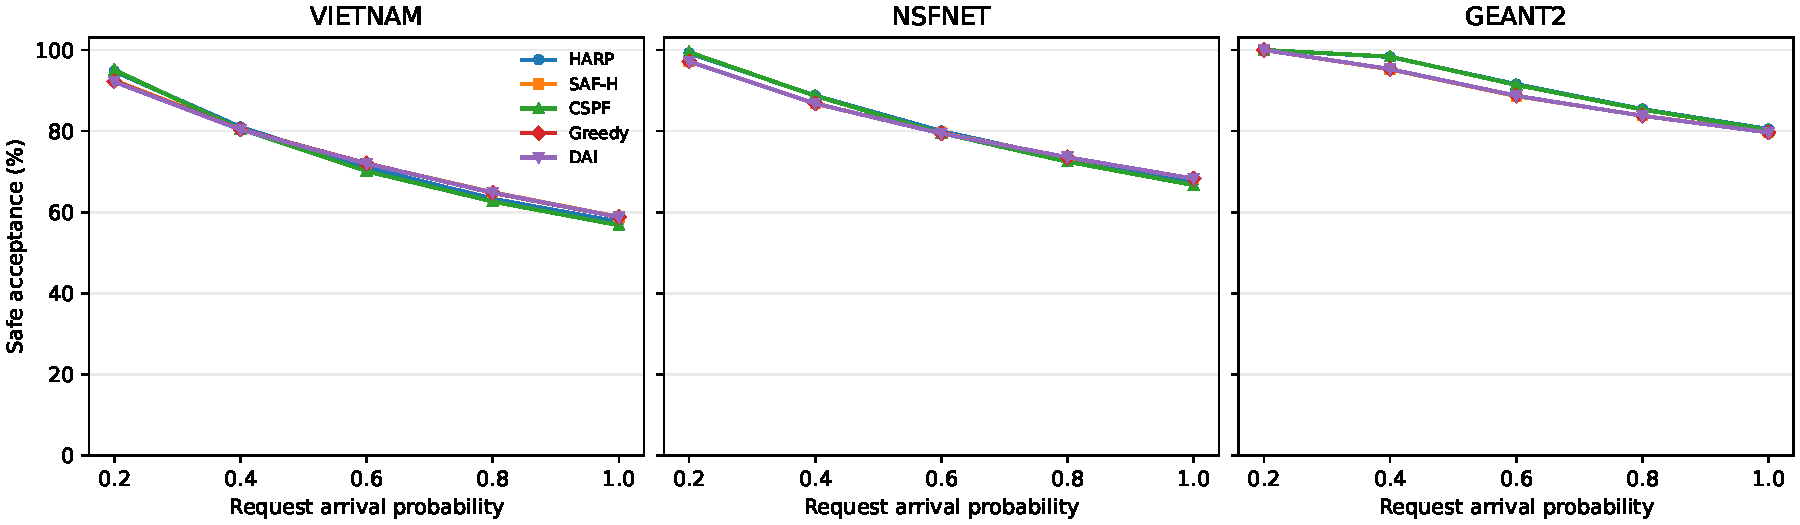
\includegraphics[width=0.94\textwidth]{figs/arrival_rate_only.pdf}
\caption{\newrev{Safe acceptance under a fixed-profile arrival-rate sweep. Arrival probability varies while the Bursty demand profile, request resource demands, requested SID depth, TTL range, topology, and policy checkpoints remain fixed. Points summarize 20 matched evaluation seeds.}}
\label{fig:arrival_rate_only}
\end{figure*}
\newrev{The paired HARP--SAF-H contrast changes direction with topology and load. HARP is higher at arrival probabilities 0.2 and 0.4 on Vietnam, at 0.2--0.6 on NSFNET, and at 0.4--1.0 on GEANT2; SAF-H is higher in the remaining non-ceiling cells. The largest mean HARP advantage is 3.067 percentage points (GEANT2, 0.4), while the largest SAF-H advantage is 1.593 points (Vietnam, 0.8). Fourteen of the 15 exact paired signed-rank comparisons remain significant after Holm correction across the 15 cells. GEANT2 at 0.2 is ceiling-limited (HARP 100.00\%, SAF-H 99.98\%; 18/20 paired differences are zero) and is not significant. These are fixed-checkpoint comparisons conditional on the simulator and matched traces, not variation across independently trained policies.}
\newrev{The separate load-sweep protocol evaluates four protected algorithms at seven combined offered-intensity multipliers from 0.2 to 1.5 on the same three topologies, using 20 seeds and 3,000 simulator steps per seed and multiplier. At multipliers up to 1.0, the multiplier sets request-arrival probability. Above 1.0, arrival probability is capped at 1.0 while CPU/RAM demand, requested SID depth, and TTL are scaled. This combined protocol therefore does not isolate arrival rate.}

\newrev{At zero background chains, the experiment comprises 4,200 seed-level policy trials across three substrates, seven intensities, and ten policy and admission configurations (five policies, protected and unprotected). The main figure presents four protected policies; the table additionally reports CSPF. Figure~\ref{fig:load_sweep} compares four protected policies and Table~\ref{tab:load_sweep_results} reports their safe acceptance at every intensity. No protected trial admitted a modeled hard violation. All 20 seeds at each topology and intensity used the same offered trace, so the reported variation is conditional on that trace.}

\newrev{For the 21 HARP--SAF-H contrasts in the combined offered-intensity experiment, paired percentile-bootstrap intervals use 20,000 resamples. The exact two-sided signed-rank test drops zero differences and assigns average ranks to tied absolute differences. Zero-difference counts, effective sample sizes, and rank-biserial effects are reported; all 21 contrasts remain in the Holm family. Appendix Table~\ref{tab:load_sweep_paired_statistics} reports these contrasts. Appendix Tables~\ref{tab:load_sweep_unprotected}--\ref{tab:load_sweep_unprotected_geant2} report modeled violations with admission disabled.}

\begin{figure*}[t]
\centering
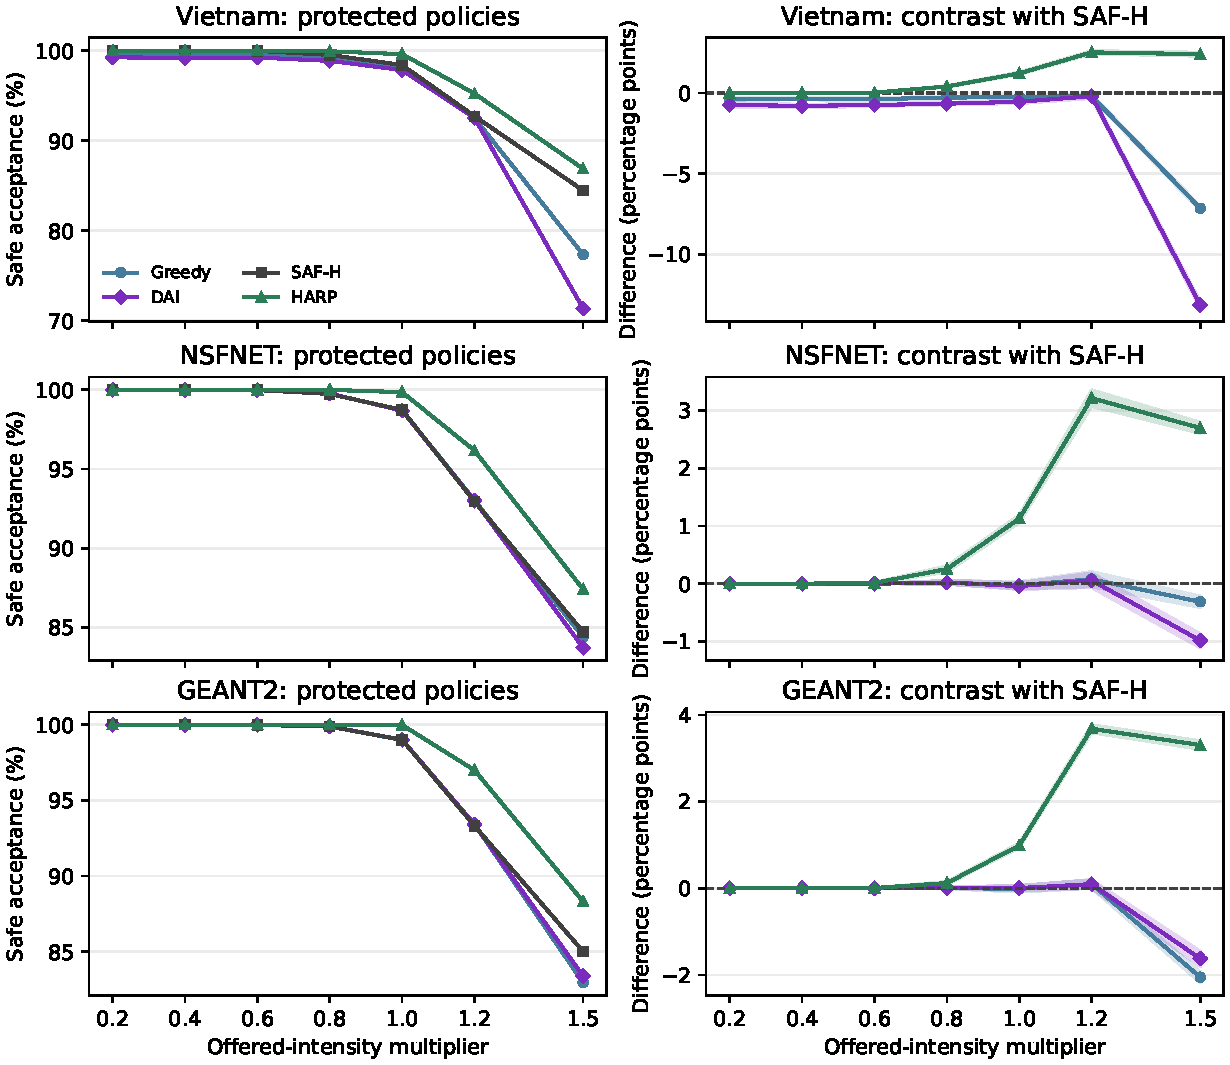
\includegraphics[width=0.97\textwidth]{figs/load_sweep_three_topologies.pdf}
\caption{\newrev{Offered-intensity sweep across Vietnam, NSFNET, and GEANT2. Left panel shows mean safe acceptance over 20 seeds. The right panel shows paired safe-acceptance differences relative to SAF-H with bootstrap 95\% intervals. The offered-intensity multiplier changes arrival probability up to 1.0 and scales demand, requested SID depth, and TTL above 1.0; this is not a pure arrival-rate sweep. All protected admitted hard-violation rates were zero.}}
\label{fig:load_sweep}
\end{figure*}

\begin{table}[t]
\centering
\caption{\newrev{Protected-policy safe acceptance across the load sweep (\%; mean $\pm$ sample SD, 20 seeds). Load denotes offered intensity; DAI denotes Decoupled AI.}}
\label{tab:load_sweep_results}
\scriptsize
{\color{revisiongreen}
\setlength{\tabcolsep}{3pt}
\resizebox{\columnwidth}{!}{%
\begin{tabular}{llrrrrr}
\toprule
Network & Load & Greedy & DAI & SAF-H & CSPF & HARP \\
\midrule
Vietnam & 0.2 & 99.62 $\pm$ 0.20 & 99.26 $\pm$ 0.32 & 100.00 $\pm$ 0.00 & 100.00 $\pm$ 0.00 & 100.00 $\pm$ 0.00 \\
Vietnam & 0.4 & 99.65 $\pm$ 0.17 & 99.20 $\pm$ 0.24 & 100.00 $\pm$ 0.02 & 100.00 $\pm$ 0.00 & 100.00 $\pm$ 0.00 \\
Vietnam & 0.6 & 99.60 $\pm$ 0.22 & 99.24 $\pm$ 0.23 & 99.98 $\pm$ 0.04 & 100.00 $\pm$ 0.00 & 100.00 $\pm$ 0.00 \\
Vietnam & 0.8 & 99.24 $\pm$ 0.20 & 98.87 $\pm$ 0.14 & 99.53 $\pm$ 0.12 & 99.91 $\pm$ 0.06 & 99.93 $\pm$ 0.07 \\
Vietnam & 1.0 & 98.14 $\pm$ 0.19 & 97.85 $\pm$ 0.25 & 98.40 $\pm$ 0.18 & 99.61 $\pm$ 0.07 & 99.61 $\pm$ 0.08 \\
Vietnam & 1.2 & 92.52 $\pm$ 0.25 & 92.52 $\pm$ 0.29 & 92.72 $\pm$ 0.19 & 95.38 $\pm$ 0.17 & 95.23 $\pm$ 0.21 \\
Vietnam & 1.5 & 77.33 $\pm$ 0.26 & 71.35 $\pm$ 0.46 & 84.47 $\pm$ 0.23 & 86.86 $\pm$ 0.29 & 86.88 $\pm$ 0.24 \\
NSFNET & 0.2 & 100.00 $\pm$ 0.00 & 100.00 $\pm$ 0.00 & 100.00 $\pm$ 0.00 & 100.00 $\pm$ 0.00 & 100.00 $\pm$ 0.00 \\
NSFNET & 0.4 & 100.00 $\pm$ 0.00 & 100.00 $\pm$ 0.00 & 100.00 $\pm$ 0.00 & 100.00 $\pm$ 0.00 & 100.00 $\pm$ 0.00 \\
NSFNET & 0.6 & 99.99 $\pm$ 0.03 & 99.99 $\pm$ 0.03 & 99.99 $\pm$ 0.03 & 100.00 $\pm$ 0.00 & 100.00 $\pm$ 0.00 \\
NSFNET & 0.8 & 99.76 $\pm$ 0.11 & 99.76 $\pm$ 0.10 & 99.74 $\pm$ 0.13 & 99.99 $\pm$ 0.02 & 99.99 $\pm$ 0.02 \\
NSFNET & 1.0 & 98.70 $\pm$ 0.17 & 98.69 $\pm$ 0.17 & 98.73 $\pm$ 0.16 & 99.84 $\pm$ 0.05 & 99.86 $\pm$ 0.06 \\
NSFNET & 1.2 & 93.03 $\pm$ 0.16 & 93.00 $\pm$ 0.16 & 92.95 $\pm$ 0.29 & 96.21 $\pm$ 0.18 & 96.16 $\pm$ 0.24 \\
NSFNET & 1.5 & 84.40 $\pm$ 0.25 & 83.73 $\pm$ 0.33 & 84.71 $\pm$ 0.16 & 87.37 $\pm$ 0.27 & 87.41 $\pm$ 0.22 \\
GEANT2 & 0.2 & 100.00 $\pm$ 0.00 & 100.00 $\pm$ 0.00 & 100.00 $\pm$ 0.00 & 100.00 $\pm$ 0.00 & 100.00 $\pm$ 0.00 \\
GEANT2 & 0.4 & 100.00 $\pm$ 0.00 & 100.00 $\pm$ 0.00 & 100.00 $\pm$ 0.00 & 100.00 $\pm$ 0.00 & 100.00 $\pm$ 0.00 \\
GEANT2 & 0.6 & 99.99 $\pm$ 0.02 & 99.99 $\pm$ 0.02 & 99.99 $\pm$ 0.02 & 100.00 $\pm$ 0.00 & 100.00 $\pm$ 0.00 \\
GEANT2 & 0.8 & 99.89 $\pm$ 0.07 & 99.89 $\pm$ 0.07 & 99.88 $\pm$ 0.08 & 100.00 $\pm$ 0.00 & 100.00 $\pm$ 0.00 \\
GEANT2 & 1.0 & 98.99 $\pm$ 0.13 & 99.01 $\pm$ 0.12 & 99.00 $\pm$ 0.13 & 99.98 $\pm$ 0.03 & 99.99 $\pm$ 0.02 \\
GEANT2 & 1.2 & 93.42 $\pm$ 0.24 & 93.42 $\pm$ 0.24 & 93.32 $\pm$ 0.24 & 97.06 $\pm$ 0.16 & 97.00 $\pm$ 0.21 \\
GEANT2 & 1.5 & 82.96 $\pm$ 0.26 & 83.39 $\pm$ 0.31 & 85.01 $\pm$ 0.22 & 88.36 $\pm$ 0.23 & 88.31 $\pm$ 0.27 \\
\bottomrule
\end{tabular}%
}}
\end{table}

\newrev{In the offered-intensity evaluation, HARP's safe-acceptance advantage over SAF-H at intensity 1.2 was 2.515, 3.213, and 3.680 percentage points on Vietnam, NSFNET, and GEANT2, respectively. At intensity 1.5, the differences were 2.402, 2.697, and 3.303 points. Appendix Table~\ref{tab:load_sweep_paired_statistics} reports paired confidence intervals and Holm-adjusted tests. These estimates are conditional on fixed N² checkpoints and the offered workload, not independently trained policy populations.}

\newrev{Acceptance is substantially higher under the shorter, topology-scaled TTL protocol than in the three-workload stress benchmark. The favorable sweep results therefore identify a workload regime in which HARP improves safe acceptance relative to SAF-H; they do not establish an advantage under long-lived stress traffic or explain individual rejections as globally infeasible.}

\newrev{To quantify rejected choices with feasible alternatives, we exhaustively evaluated the simulator's complete 10-node pair-action space at sampled decision states. For each of 10 seeds, 120 states were sampled at a stride of 25 from a 3,000-step Bursty run. Every one of the 100 placement--routing pairs was replayed from the same pre-decision snapshot through the simulator step, including its TTL-expiration phase before admission. In the Vietnam oracle experiment, HARP selected a rejected action at 583/1,200 sampled states; 30 had an alternative accepted by the same simulator predicate. The per-seed rate of such alternatives among HARP's selected rejections averaged 5.16\% (sample SD 1.84\%). SAF-H had 579/1,200 selected rejections, of which 33 had an accepted alternative; the corresponding mean was 5.70\% (sample SD 2.32\%). These descriptive rates do not use sampled decisions as independent replicates; policy trajectories also differ. They identify avoidable choices in the simulator's pair space, not live-network or full-chain feasibility.}

\begin{table*}[t]
\centering
\caption{\newrev{Sampled exhaustive pair-action oracle on Vietnam (10 seeds; 120 states per seed). Conditional rates are seed-level means with sample SD.}}
\label{tab:missed_feasible_oracle}
\scriptsize
{\color{revisiongreen}
\setlength{\tabcolsep}{3pt}
\resizebox{\textwidth}{!}{%
\begin{tabular}{lrrrr}
\toprule
Policy & Sampled states & Selected rejections & With accepted alternative & Conditional rate (\%; mean $\pm$ SD) \\
\midrule
HARP & 1,200 & 583 & 30 & 5.16 $\pm$ 1.84 \\
SAF-H & 1,200 & 579 & 33 & 5.70 $\pm$ 2.32 \\
\bottomrule
\end{tabular}%
}}
\end{table*}

\newrev{A separate active-chain experiment initializes 0, 25, 50, or 100 long-lived background chains before each 3,000-step Bursty evaluation. Each chain reserves 2 CPU units, 2 RAM units, and 20 bandwidth units, with round-robin placement. The run covers 20 seeds and all four protected algorithms on Vietnam, NSFNET, and GEANT2. Table~\ref{tab:active_chain_stress} compares protected HARP, SAF-H, and CSPF; the reported values are mean safe acceptance with sample standard deviation across seeds. Admitted modeled hard violations were zero for all protected algorithms in every tested condition. HARP's safe acceptance declined as background occupancy increased, while remaining above SAF-H in these simulator conditions.}

{\color{revisiongreen}
\begin{table}[t]
\centering
\caption{Safe acceptance under long-lived background-chain occupancy (20 seeds; mean $\pm$ sample SD, percentages).}
\label{tab:active_chain_stress}
\scriptsize
\setlength{\tabcolsep}{3pt}
\resizebox{\columnwidth}{!}{%
\begin{tabular}{lrrrr}
\toprule
Network & Chains & HARP & SAF-H & CSPF \\
\midrule
Vietnam & 0 & 99.61 $\pm$ 0.08 & 98.40 $\pm$ 0.18 & 99.61 $\pm$ 0.07 \\
Vietnam & 25 & 99.19 $\pm$ 0.10 & 97.62 $\pm$ 0.18 & 99.21 $\pm$ 0.11 \\
Vietnam & 50 & 98.55 $\pm$ 0.15 & 96.69 $\pm$ 0.23 & 98.59 $\pm$ 0.15 \\
Vietnam & 100 & 97.08 $\pm$ 0.13 & 94.38 $\pm$ 0.17 & 97.00 $\pm$ 0.15 \\
NSFNET & 0 & 99.86 $\pm$ 0.06 & 98.73 $\pm$ 0.16 & 99.84 $\pm$ 0.05 \\
NSFNET & 25 & 99.73 $\pm$ 0.10 & 98.19 $\pm$ 0.15 & 99.72 $\pm$ 0.10 \\
NSFNET & 50 & 99.47 $\pm$ 0.12 & 97.56 $\pm$ 0.14 & 99.40 $\pm$ 0.10 \\
NSFNET & 100 & 98.62 $\pm$ 0.14 & 95.96 $\pm$ 0.19 & 98.64 $\pm$ 0.14 \\
GEANT2 & 0 & 99.99 $\pm$ 0.02 & 99.00 $\pm$ 0.13 & 99.98 $\pm$ 0.03 \\
GEANT2 & 25 & 99.99 $\pm$ 0.03 & 98.75 $\pm$ 0.16 & 99.97 $\pm$ 0.03 \\
GEANT2 & 50 & 99.94 $\pm$ 0.05 & 98.47 $\pm$ 0.12 & 99.91 $\pm$ 0.06 \\
GEANT2 & 100 & 99.79 $\pm$ 0.08 & 97.69 $\pm$ 0.18 & 99.79 $\pm$ 0.10 \\
\bottomrule
\end{tabular}%
}
\end{table}
}

\newrev{We additionally evaluated the size-matched HARP checkpoints on synthetic 25-, 50-, and 100-node topologies. Table~\ref{tab:synthetic_stress} reports safe acceptance in the same three stress workloads, with 20 evaluation seeds and 3,000 offered requests per seed. These fixed-checkpoint simulator results quantify workload-specific acceptance; they do not measure independent training variability or physical deployment.}
\begin{table*}[t]
\centering
\caption{Protected safe acceptance on synthetic topologies (percent; mean $\pm$ sample SD across 20 seeds). E, B, and C denote Elephant stress, Burst surge, and Chaos.}
\label{tab:synthetic_stress}
\scriptsize
\begin{tabular}{llrrrrr}
\toprule
Nodes & Profile & Greedy & DAI & SAF-H & CSPF & HARP \\
\midrule
25 & E & 66.45 $\pm$ 0.38 & 66.45 $\pm$ 0.38 & 66.51 $\pm$ 0.37 & 66.52 $\pm$ 0.36 & 66.76 $\pm$ 0.54 \\
25 & B & 81.35 $\pm$ 0.27 & 81.35 $\pm$ 0.27 & 81.35 $\pm$ 0.25 & 81.35 $\pm$ 0.25 & 82.62 $\pm$ 0.44 \\
25 & C & 68.56 $\pm$ 0.47 & 68.56 $\pm$ 0.47 & 68.44 $\pm$ 0.41 & 68.45 $\pm$ 0.41 & 68.33 $\pm$ 0.58 \\
50 & E & 79.98 $\pm$ 0.23 & 79.99 $\pm$ 0.22 & 79.97 $\pm$ 0.24 & 79.99 $\pm$ 0.23 & 83.67 $\pm$ 0.34 \\
50 & B & 93.37 $\pm$ 0.25 & 93.35 $\pm$ 0.31 & 93.35 $\pm$ 0.19 & 93.33 $\pm$ 0.17 & 97.64 $\pm$ 0.23 \\
50 & C & 82.06 $\pm$ 0.27 & 82.08 $\pm$ 0.28 & 82.03 $\pm$ 0.28 & 82.06 $\pm$ 0.31 & 85.70 $\pm$ 0.28 \\
100 & E & 92.66 $\pm$ 0.27 & 92.65 $\pm$ 0.26 & 92.64 $\pm$ 0.30 & 92.66 $\pm$ 0.29 & 98.84 $\pm$ 0.30 \\
100 & B & 100.00 $\pm$ 0.01 & 100.00 $\pm$ 0.01 & 100.00 $\pm$ 0.01 & 100.00 $\pm$ 0.01 & 100.00 $\pm$ 0.00 \\
100 & C & 92.36 $\pm$ 0.34 & 92.36 $\pm$ 0.27 & 92.47 $\pm$ 0.33 & 92.44 $\pm$ 0.35 & 99.57 $\pm$ 0.20 \\
\bottomrule
\end{tabular}
\end{table*}

\begin{table*}[t]
\centering
\caption{Exploratory HARP minus strongest protected baseline safe acceptance (percentage points; 20 paired seeds). The strongest baseline is selected by sample mean in the same cell. $p_H$ uses Holm correction over nine real-topology comparisons; selection uncertainty is not accounted for.}
\label{tab:best_baseline_exploratory}
\scriptsize
\begin{tabular}{lllrrrr}
\toprule
Network & Profile & Baseline & $\Delta$ & 95\% CI & $p_H$ & $n_{eff}$ \\
\midrule
Vietnam & E & SAF-H & -1.335 & [-1.603, -1.052] & 2.29e-05 & 20 \\
Vietnam & B & SAF-H & -1.185 & [-1.338, -1.028] & 1.72e-05 & 20 \\
Vietnam & C & SAF-H & -1.108 & [-1.273, -0.948] & 1.72e-05 & 20 \\
NSFNET & E & SAF-H & -0.540 & [-0.715, -0.368] & 3.81e-05 & 19 \\
NSFNET & B & SAF-H & -0.868 & [-1.052, -0.685] & 1.72e-05 & 20 \\
NSFNET & C & SAF-H & -0.842 & [-1.057, -0.623] & 3.81e-05 & 20 \\
GEANT2 & E & Greedy & 0.043 & [-0.115, 0.200] & 0.564 & 20 \\
GEANT2 & B & CSPF & 0.183 & [0.042, 0.327] & 0.142 & 20 \\
GEANT2 & C & SAF-H & -0.242 & [-0.455, -0.030] & 0.0751 & 19 \\
\bottomrule
\end{tabular}
\end{table*}

\newrev{Table~\ref{tab:best_baseline_exploratory} compares HARP with the strongest protected baseline in each real-topology workload cell. This comparison is exploratory because the baseline is selected using the same evaluation seeds; the interval and corrected $p$ values do not account for selection.}

\newrev{A further audit follows the corrected HARP checkpoint over 20 Bursty stress seeds per topology and cross-tabulates pre-decision mask emptiness with the subsequent admission outcome (Table~\ref{tab:mask_ttl_audit}). No rejection occurred when the mask was nonempty in these 180,000 offered decisions. The mask is computed before the simulator advances TTL; when the same state is inspected after pending expiry, some previously empty masks contain feasible pairs. This counterfactual does not change the executed action or establish the outcome of a post-expiry policy.}
\begin{table}[t]
\centering
\caption{Pre-step mask and admission audit: 20 seeds and 60,000 decisions per topology. Last column counts empty masks becoming nonempty after pending TTL expiry.}
\label{tab:mask_ttl_audit}
\scriptsize
\resizebox{\columnwidth}{!}{%
\begin{tabular}{lrrrr}
\toprule
Network & Empty & Rejected, empty & Rejected, nonempty & Empty $\rightarrow$ nonempty \\
\midrule
Vietnam & 25547 & 25406 & 0 & 1422 \\
NSFNET & 19591 & 19554 & 0 & 971 \\
GEANT2 & 11750 & 11708 & 0 & 556 \\
\bottomrule
\end{tabular}}
\end{table}

\newrev{We then ran a separate simulator intervention for 20 Bursty seeds per topology. It selects the action using a mask computed after the pending TTL expiry, while retaining the pre-expiry observation; the simulator transition and runtime code are unchanged. Each intervention run shares its offered trace with the current-policy run, and every current-policy safe-acceptance value matches the benchmark seed record. Mean paired changes in safe acceptance were +0.065 percentage points on Vietnam (95\% bootstrap CI [-0.143, 0.265]), -0.005 on NSFNET ([-0.187, 0.182]), and +0.085 on GEANT2 ([-0.045, 0.220]); Holm-adjusted Wilcoxon $p$ values were 0.938, 0.938, and 0.787. The CIs include zero and the policy trajectories diverge after changed actions. This evidence does not justify reporting a systematic acceptance gain from changing TTL/mask order; the evaluated runtime therefore retains its original state-transition order.}

\newrev{To check the repeated Bursty trace limitation, a supplementary experiment offsets the input dataset by a seed-dependent amount while retaining the same Bursty schedule. All five protected policies share the offered trace within each seed; results cover 20 seeds per topology, and the same intervention was evaluated over the load and background-chain protocols. These are additional simulator workloads and do not estimate variation across independent policy training runs. In this seed-offset stress comparison, mean safe acceptance for HARP and SAF-H was 57.37\% and 58.75\% on Vietnam, 67.55\% and 68.47\% on NSFNET, and 80.42\% and 79.70\% on GEANT2, respectively.}

\newrev{For SAF-H weight sensitivity, we doubled each of the latency, CPU-utilization, and hop coefficients separately, keeping the other coefficients fixed. Across these four settings, mean safe acceptance ranged from 92.67--92.72\% on Vietnam, 92.95\% on NSFNET, and 93.32\% on GEANT2 at intensity 1.2; at intensity 1.5, the corresponding ranges were 84.47--84.65\%, 84.68--84.72\%, and 85.01--85.08\%. These exploratory ranges use 20 matched seeds and do not establish robustness to all weight choices.}

\newrev{We also evaluated the existing Full and MLP ablation checkpoints on a symmetric three-nearest-neighbour adjacency constructed from pair latency. Table~\ref{tab:sparse_gat_mlp} reports matched-seed safe acceptance. The GAT adjacency is replaced at evaluation time; the policies were not retrained on this graph. The adjacency is synthetic, and the simulator does not establish physical multihop forwarding.}
\begin{table}[t]
\centering
\caption{Full GAT versus MLP under synthetic sparse adjacency (20 matched Bursty seeds; safe acceptance percent, paired difference in percentage points with 95\% bootstrap CI).}
\label{tab:sparse_gat_mlp}
\scriptsize
\resizebox{\columnwidth}{!}{%
\begin{tabular}{lrrrr}
\toprule
Network & Full & MLP & Difference & 95\% CI \\
\midrule
Vietnam & 56.87 & 57.27 & -0.398 & [-0.572, -0.235] \\
NSFNET & 67.05 & 66.87 & 0.178 & [-0.027, 0.377] \\
GEANT2 & 80.55 & 80.63 & -0.080 & [-0.233, 0.072] \\
\bottomrule
\end{tabular}}
\end{table}

\newrev{We extended the sampled pair oracle to offered intensities 1.2 and 1.5 across the three topologies (Table~\ref{tab:oracle_load_followup}). Each policy uses ten seeds and 120 sampled decisions per seed. Accepted alternatives are conditional on the simulator snapshot and TTL-expiry transition; the policies may follow different trajectories.}
\begin{table}[t]
\centering
\caption{Sampled pair oracle for the offered-intensity protocol. Counts aggregate ten seeds; sampled states are not independent replications.}
\label{tab:oracle_load_followup}
\scriptsize
\resizebox{\columnwidth}{!}{%
\begin{tabular}{llrrrr}
\toprule
Network & Load & Policy & States & Rejected & With alternative \\
\midrule
Vietnam & 1.2 & HARP & 1200 & 52 & 8 \\
Vietnam & 1.2 & SAF-H & 1200 & 89 & 13 \\
Vietnam & 1.5 & HARP & 1200 & 156 & 23 \\
Vietnam & 1.5 & SAF-H & 1200 & 211 & 19 \\
NSFNET & 1.2 & HARP & 1200 & 52 & 4 \\
NSFNET & 1.2 & SAF-H & 1200 & 81 & 16 \\
NSFNET & 1.5 & HARP & 1200 & 172 & 13 \\
NSFNET & 1.5 & SAF-H & 1200 & 211 & 21 \\
GEANT2 & 1.2 & HARP & 1200 & 45 & 7 \\
GEANT2 & 1.2 & SAF-H & 1200 & 97 & 16 \\
GEANT2 & 1.5 & HARP & 1200 & 168 & 17 \\
GEANT2 & 1.5 & SAF-H & 1200 & 211 & 20 \\
\bottomrule
\end{tabular}}
\end{table}

\subsection{\newrev{Decision Cost and Topology Scaling}}
\label{subsec:decision_cost}
\newrev{A separate serialized, same-process Vietnam policy-decision timing study used the Bursty workload, 10 matched seeds, and 3,000 steps per seed. This controlled study uses a separately pinned HARP checkpoint; the size-matched main-policy measurements are reported separately in Table~\ref{tab:harp_component_timing}. Per-seed offered-trace hashes matched exactly between HARP and SAF-H. After one excluded warm-up run per policy, execution order alternated across seeds. Mean seed-level decision P50/P95/P99 was 1.925/2.131/2.481~ms for HARP and 0.339/0.494/0.527~ms for SAF-H; HARP's P95 was 1.637~ms higher (4.3$\times$). HARP's mean seed-level policy-inference P95 was 1.617~ms. For SAF-H, feasible-set construction and heuristic selection had mean seed-level P95 values of 0.062 and 0.133~ms. The measured simulator runners processed 537 and 3,282 offered decisions per second, respectively, calculated from completed simulator decisions and run wall time. The decision intervals include the simulator step and exclude live telemetry transport, controller handoff, deployment, readiness, and steering.}

\newrev{For the size-matched HARP stress benchmark, Table~\ref{tab:harp_component_timing} reports means of seed-level P95 timings for normalization, mask construction, policy inference, and total simulator decision time in the Burst-surge profile. Benchmark jobs ran concurrently on a shared host; these measurements are not isolated latency measurements. Components can overlap and their P95 values cannot be added to obtain total P95.}
\begin{table}[t]
\centering
\caption{HARP simulator timing in synthetic Burst-surge runs (ms; mean of 20 seed-level P95 values).}
\label{tab:harp_component_timing}
\scriptsize
\resizebox{\columnwidth}{!}{%
\begin{tabular}{rrrrr}
\toprule
Nodes & Normalize & Mask & Inference & Decision \\
\midrule
25 & 0.067 & 0.550 & 3.948 & 5.378 \\
50 & 0.074 & 2.022 & 10.831 & 13.642 \\
100 & 0.056 & 6.659 & 19.118 & 26.101 \\
\bottomrule
\end{tabular}}
\end{table}

\newrev{Topology-size timing was measured for SAF-H on deterministic synthetic grids with 25, 50, and 100 nodes, 10 seeds, and 300 decisions per seed; the complete pair-action space contains $N^2$ candidates. Mean per-seed feasible-set P50/P95/P99 time was 0.315/0.368/0.390~ms, 1.355/1.488/1.649~ms, and 5.534/70.175/76.377~ms, respectively. Mean per-seed decision P95/P99 was 1.554/1.620, 5.297/5.728, and 83.562/89.829~ms. The 100-node feasible-set P95 ranged from 68.441 to 72.238~ms across the ten seeds, versus a P50 range of 5.510--5.563~ms; the corresponding decision P95 range was 81.643--85.574~ms. Thus the tail recurred within every seed and was concentrated in feasible-set construction, rather than being a single anomalous seed. The saved percentiles cannot identify which suboperation or host condition within that construction caused the tail. These measurements characterize SAF-H's simulator-side scaling on synthetic grids; HARP decision timings are reported for the evaluated benchmark topologies. The synthetic-grid SAF-H timing runs were serial with no pre-seeded background chains; the evaluated implementations did not use a candidate-path cache. Live API concurrency and campaign actuation latency are reported separately in Section~\ref{subsec:testbed_validation}.}

\begin{table}[t]
\centering
\caption{\newrev{SAF-H timing versus synthetic topology size (10 seeds; 300 decisions per seed). Values are means of seed-level percentiles.}}
\label{tab:synthetic_scalability}
\scriptsize
{\color{revisiongreen}
\setlength{\tabcolsep}{3pt}
\resizebox{\columnwidth}{!}{%
\begin{tabular}{rrrrrr}
\toprule
Nodes & Links & Pair actions ($N^2$) & Feasible-set P50 (ms) & Feasible-set P95 (ms) & Decision P95 (ms) \\
\midrule
25 & 40 & 625 & 0.315 & 0.368 & 1.554 \\
50 & 85 & 2,500 & 1.355 & 1.488 & 5.297 \\
100 & 180 & 10,000 & 5.534 & 70.175 & 83.562 \\
\bottomrule
\end{tabular}%
}}
\end{table}

\begin{figure*}[t]
    \centering
    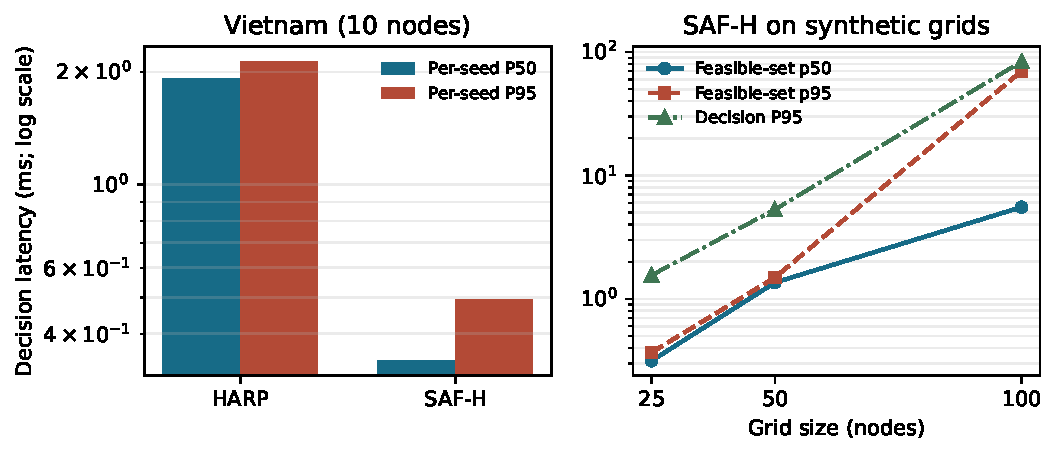
\includegraphics[width=0.92\textwidth]{figs/policy_cost_scalability.pdf}
    \caption{\newrev{Measured simulator decision latency and SAF-H topology-size cost. Left: mean per-seed decision P50 and P95 for HARP and SAF-H on Vietnam (10 seeds, 3,000 steps per seed). Right: mean per-seed feasible-set P50 and P95 and decision P95 for SAF-H on synthetic 25-, 50-, and 100-node grids (10 seeds, 300 decisions per seed). Axes use a logarithmic scale. Measurements cover local simulator decisions.}}
    \label{fig:policy_cost_scalability}
\end{figure*}

\newrev{The simulator measurements characterize policy-decision processing. The 12-hour control-plane HIL separately reports API response latency and Kubernetes baseline readiness. In the end-to-end campaign, submission to steering confirmation took \HILEtoESubmitSteerPF{}/\HILEtoESubmitSteerPNF{}~s at P50/P95 and was dominated by Tekton deployment and Pod readiness, not by policy computation.}

\paragraph{Variation across independently trained policies.}
\newrev{To distinguish training variation from evaluation-seed variation, we trained Vietnam HARP with seeds 42, 7, and 2024 at the same nominal two-million-transition budget. All three final checkpoints contain 2,002,944 transitions. Each model is evaluated deterministically over the same 20 Bursty stress seeds and 3,000 offered requests per seed, using its own frozen observation normalizer. Appendix Table~\ref{tab:independent_training} reports the model-specific mean and evaluation-seed SD. Model means range from \TrainingMeanMin{}\% to \TrainingMeanMax{}\%, with sample SD \TrainingMeanSD{} percentage points across the three model means. This descriptive check estimates training variation for Vietnam under this workload; it does not extend the training-seed analysis to other topologies.}

\subsection{\newrev{Operational Interpretation, Overhead, and Limitations}}
\label{subsec:operational_interpretation}
\newrev{The policy comparison depends on workload and resource pressure. SAF-H achieves higher acceptance in all six Vietnam and NSFNET stress conditions, and in GEANT2 Chaos; HARP improves GEANT2 Burst-surge acceptance by 0.808 percentage points, while the Elephant-stress difference is inconclusive. The fixed-profile arrival-rate experiment also shows direction changes across topologies and rates, while the combined offered-intensity and background-occupancy protocols favor HARP in their tested conditions. These complementary results support workload-specific policy selection through a common admission interface.}

\newrev{Acceptance gains must also be weighed against computation. In the Vietnam ablation, the MLP variant achieves slightly higher mean safe acceptance and lower mean seed-level decision P95 than the full GAT policy under both Uniform and Bursty traffic (Figure~\ref{fig:ablation_cost}). In the controlled HARP--SAF-H comparison, HARP's mean decision P95 was 4.3 times SAF-H's, while the HARP policy-inference component alone averaged 1.617~ms at P95. The measured advantage therefore depends on the workload regime and carries a local computation cost; the evidence supports policy choice through a common admission boundary, not a general efficiency advantage.}

\newrev{Appendix Table~\ref{tab:stress_qos} reports service latency and SLA outcomes for HARP and SAF-H by workload. Across the nine stress conditions, mean seed-level simulated service latency is 5.25--7.39~ms for HARP and 0.32--0.62~ms for SAF-H; mean seed-level SLA-violation rates are approximately 0.00--0.21\% and zero, respectively. These quantities describe the requests admitted by each policy, whose composition may differ. SAF-H may choose the same node for placement and routing. HARP also permits that pair but its reward includes a bonus for distinct endpoints. They provide no evidence of a HARP service-latency advantage in these conditions and are distinct from policy-computation timing.}

\newrev{The evaluation uses latency-derived graphs and synthetic demand; the named substrate graphs are complete at the chosen thresholds. Main policy comparisons are conditional on topology-specific checkpoints; the three-training-seed check covers Vietnam only. The primary Bursty sweeps share an offered trace, supplemented by a seed-offset sensitivity study. MSD-invalid proposals are infrequent in simulation. Shared-host HARP timings include scheduling effects. HIL measurements concern one VNF per request on BMv2, with the recorded runtime network configuration. They establish deployment, rule readback, steering, packet delivery, and migration ordering under the tested conditions. Ordered multi-VNF traversal, ASIC behavior, flow continuity during migration, and Hybrid switching performance are outside this measurement scope.}

\section{Conclusion}
\label{sec:conclusion}
\newrev{AIO-Mesh connects policy proposals to a fail-closed admission and actuation path for programmable cloud-native infrastructure. The common admission boundary rejected modeled hard-invalid proposals from both learned and heuristic policies; the MSD-bypass ablations exposed 9 and 182 admitted MSD-invalid actions over 720,000 simulator decisions per variant. On BMv2, admitted single-VNF paths were associated with deployment, rule readback, steering confirmation, and packet probes. Controlled over-depth traffic was dropped at the first switch whose configured MSD was exceeded. The 12-hour control-plane run completed \HILRequests{} requests without timeout, while both three-hour runs delivered 1,800/1,800 probes to previously steered VNFs; the released-capacity run accepted 209/3,083 admission requests.}

\newrev{Policy effectiveness varied with workload and topology. SAF-H generally led in the long-lived stress benchmark. The fixed-profile arrival-rate experiment showed paired differences favoring HARP in some topology--rate conditions and SAF-H in others; the combined offered-intensity and occupancy experiments favored HARP under their tested conditions, at greater local decision cost. These results support workload-aware policy choice through a common admission interface. HIL forwarding evidence covers single-VNF requests on BMv2 and does not establish ordered multi-VNF traversal, migration flow continuity, or ASIC behavior.}

\clearpage
\section*{Appendix: Supplementary Results}
\begingroup
\setcounter{figure}{0}
\renewcommand{\thefigure}{A.\arabic{figure}}
\renewcommand{\theHfigure}{appendix.\arabic{figure}}
\setcounter{table}{0}
\renewcommand{\thetable}{A.\arabic{table}}
\renewcommand{\theHtable}{appendix.\arabic{table}}
\begin{figure*}[p]
\centering
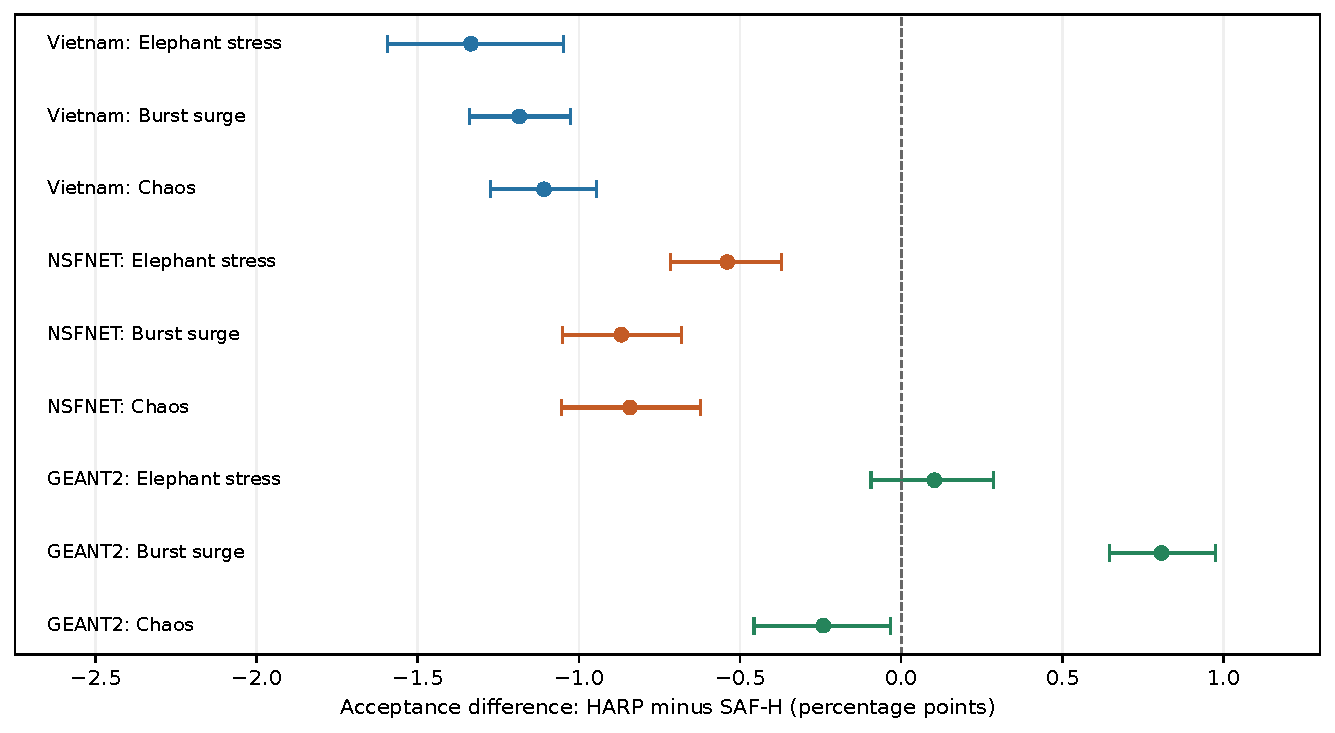
\includegraphics[width=0.94\textwidth]{figs/benchmark_paired_effects.pdf}
\caption{\newrev{Protected HARP minus SAF-H acceptance across three topologies and three stress workloads. Points show mean paired seed-level differences; horizontal intervals are percentile-bootstrap 95\% confidence intervals from paired seed-level trials. Positive values favor HARP. Holm-adjusted tests across all nine conditions are reported in Table~\ref{tab:benchmark_paired_statistics}.}}
\label{fig:benchmark_effects}
\end{figure*}

\begin{figure*}[p]
\centering
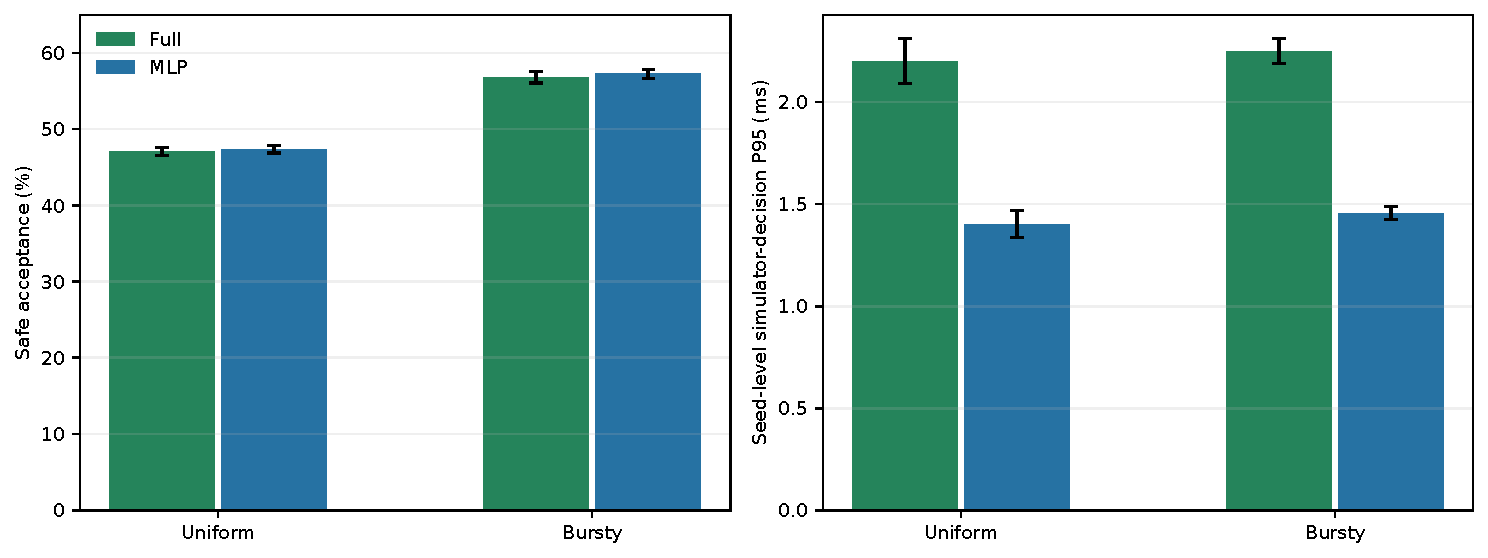
\includegraphics[width=0.94\textwidth]{figs/ablation_compute_cost.pdf}
\caption{\newrev{Acceptance and measured computation cost of Full and MLP ablation checkpoints on Vietnam. Bars show means and error bars show sample SD across 20 evaluation seeds. The right panel aggregates the per-seed P95 interval including normalization, inference, and simulator stepping; it excludes external controller actuation.}}
\label{fig:ablation_cost}
\end{figure*}

\begin{figure*}[p]
\centering
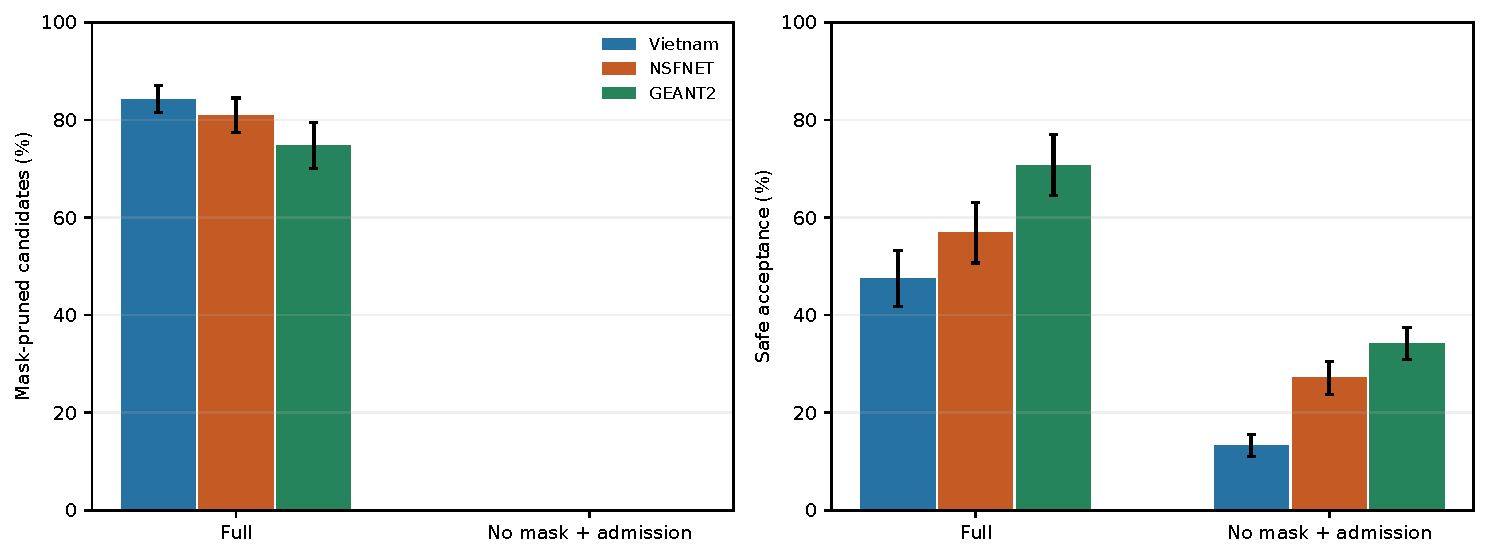
\includegraphics[width=0.94\textwidth]{figs/ablation_mask_admission.pdf}
\caption{\newrev{Candidate pruning and safe acceptance for Full and NoMask ablation variants with runtime admission enabled. Bars summarize 80 seed--workload cells per topology; error bars are sample SD across those cells. All six protected configurations recorded zero admitted hard violations. Distinct checkpoints and resulting state trajectories limit causal attribution to masking alone.}}
\label{fig:ablation_pruning}
\end{figure*}

\begin{table*}[p]
\centering
\color{revisiongreen}\small
\begin{tabular}{llrrrrrr}
\toprule
Topology & Intensity & $\Delta$ (pp) & 95\% CI & $p$ & $r_{rb}$ & $n_{eff}$ & $p_{Holm}$ \\
\midrule
VIETNAM & 0.2 & 0.000 & [0.000, 0.000] & 1 & -- & 0 & 1 \\
VIETNAM & 0.4 & 0.004 & [0.000, 0.012] & 1 & 1.000 & 1 & 1 \\
VIETNAM & 0.6 & 0.019 & [0.006, 0.038] & 0.0625 & 1.000 & 5 & 0.562 \\
VIETNAM & 0.8 & 0.401 & [0.353, 0.450] & 1.91e-06 & 1.000 & 20 & 4.01e-05 \\
VIETNAM & 1.0 & 1.213 & [1.132, 1.297] & 1.91e-06 & 1.000 & 20 & 4.01e-05 \\
VIETNAM & 1.2 & 2.515 & [2.415, 2.618] & 1.91e-06 & 1.000 & 20 & 4.01e-05 \\
VIETNAM & 1.5 & 2.402 & [2.278, 2.523] & 1.91e-06 & 1.000 & 20 & 4.01e-05 \\
NSFNET & 0.2 & 0.000 & [0.000, 0.000] & 1 & -- & 0 & 1 \\
NSFNET & 0.4 & 0.000 & [0.000, 0.000] & 1 & -- & 0 & 1 \\
NSFNET & 0.6 & 0.014 & [0.003, 0.028] & 0.125 & 1.000 & 4 & 1 \\
NSFNET & 0.8 & 0.253 & [0.201, 0.307] & 1.91e-06 & 1.000 & 20 & 4.01e-05 \\
NSFNET & 1.0 & 1.127 & [1.057, 1.190] & 1.91e-06 & 1.000 & 20 & 4.01e-05 \\
NSFNET & 1.2 & 3.213 & [3.070, 3.357] & 1.91e-06 & 1.000 & 20 & 4.01e-05 \\
NSFNET & 1.5 & 2.697 & [2.607, 2.802] & 1.91e-06 & 1.000 & 20 & 4.01e-05 \\
GEANT2 & 0.2 & 0.000 & [0.000, 0.000] & 1 & -- & 0 & 1 \\
GEANT2 & 0.4 & 0.000 & [0.000, 0.000] & 1 & -- & 0 & 1 \\
GEANT2 & 0.6 & 0.006 & [0.000, 0.014] & 0.5 & 1.000 & 2 & 1 \\
GEANT2 & 0.8 & 0.120 & [0.089, 0.154] & 3.81e-06 & 1.000 & 19 & 4.01e-05 \\
GEANT2 & 1.0 & 0.985 & [0.928, 1.040] & 1.91e-06 & 1.000 & 20 & 4.01e-05 \\
GEANT2 & 1.2 & 3.680 & [3.585, 3.770] & 1.91e-06 & 1.000 & 20 & 4.01e-05 \\
GEANT2 & 1.5 & 3.303 & [3.205, 3.403] & 1.91e-06 & 1.000 & 20 & 4.01e-05 \\
\bottomrule
\end{tabular}
\caption{Paired HARP--SAF-H safe-acceptance differences in the refreshed-model load sweep. $\Delta$ is the matched-seed mean; CI is a 20,000-resample paired percentile-bootstrap 95\% interval. $p$ is the exact two-sided Wilcoxon signed-rank test after dropping zeros and averaging tied absolute ranks; Holm correction covers all 21 topology--intensity tests.}
\label{tab:load_sweep_paired_statistics}
\end{table*}
\begin{table*}[p]
\centering
\color{revisiongreen}\small
\begin{tabular}{llrrrrr}
\toprule
Intensity & Policy & CPU & RAM & BW & MSD & Any hard violation \\
\midrule
0.2 & Greedy & 0.000 $\pm$ 0.000 & 0.000 $\pm$ 0.000 & 0.000 $\pm$ 0.000 & 0.378 $\pm$ 0.201 & 0.378 $\pm$ 0.201 \\
0.2 & DAI & 0.000 $\pm$ 0.000 & 0.000 $\pm$ 0.000 & 0.000 $\pm$ 0.000 & 0.748 $\pm$ 0.310 & 0.748 $\pm$ 0.310 \\
0.2 & SAF-H & 0.000 $\pm$ 0.000 & 0.000 $\pm$ 0.000 & 0.000 $\pm$ 0.000 & 0.865 $\pm$ 0.334 & 0.865 $\pm$ 0.334 \\
0.2 & HARP & 2.180 $\pm$ 0.662 & 0.158 $\pm$ 0.214 & 0.000 $\pm$ 0.000 & 0.000 $\pm$ 0.000 & 2.180 $\pm$ 0.662 \\
0.4 & Greedy & 0.004 $\pm$ 0.018 & 0.000 $\pm$ 0.000 & 0.000 $\pm$ 0.000 & 0.368 $\pm$ 0.139 & 0.372 $\pm$ 0.134 \\
0.4 & DAI & 0.004 $\pm$ 0.018 & 0.000 $\pm$ 0.000 & 0.000 $\pm$ 0.000 & 0.687 $\pm$ 0.198 & 0.692 $\pm$ 0.201 \\
0.4 & SAF-H & 0.004 $\pm$ 0.018 & 0.000 $\pm$ 0.000 & 0.000 $\pm$ 0.000 & 0.728 $\pm$ 0.208 & 0.732 $\pm$ 0.210 \\
0.4 & HARP & 6.853 $\pm$ 0.837 & 2.298 $\pm$ 0.689 & 0.000 $\pm$ 0.000 & 0.000 $\pm$ 0.000 & 6.853 $\pm$ 0.837 \\
0.6 & Greedy & 0.019 $\pm$ 0.037 & 0.000 $\pm$ 0.000 & 0.000 $\pm$ 0.000 & 0.289 $\pm$ 0.154 & 0.308 $\pm$ 0.170 \\
0.6 & DAI & 0.019 $\pm$ 0.037 & 0.000 $\pm$ 0.000 & 0.000 $\pm$ 0.000 & 0.698 $\pm$ 0.153 & 0.715 $\pm$ 0.158 \\
0.6 & SAF-H & 0.019 $\pm$ 0.037 & 0.000 $\pm$ 0.000 & 0.000 $\pm$ 0.000 & 0.703 $\pm$ 0.176 & 0.720 $\pm$ 0.186 \\
0.6 & HARP & 14.058 $\pm$ 1.448 & 6.322 $\pm$ 1.205 & 0.000 $\pm$ 0.000 & 0.022 $\pm$ 0.028 & 14.080 $\pm$ 1.445 \\
0.8 & Greedy & 0.508 $\pm$ 0.152 & 0.002 $\pm$ 0.009 & 0.000 $\pm$ 0.000 & 0.351 $\pm$ 0.109 & 0.845 $\pm$ 0.185 \\
0.8 & DAI & 0.509 $\pm$ 0.150 & 0.000 $\pm$ 0.000 & 0.000 $\pm$ 0.000 & 0.735 $\pm$ 0.131 & 1.206 $\pm$ 0.188 \\
0.8 & SAF-H & 0.506 $\pm$ 0.146 & 0.000 $\pm$ 0.000 & 0.000 $\pm$ 0.000 & 0.756 $\pm$ 0.145 & 1.229 $\pm$ 0.235 \\
0.8 & HARP & 27.387 $\pm$ 1.456 & 16.232 $\pm$ 1.393 & 0.000 $\pm$ 0.000 & 0.044 $\pm$ 0.044 & 27.428 $\pm$ 1.441 \\
1.0 & Greedy & 2.158 $\pm$ 0.240 & 0.005 $\pm$ 0.012 & 0.000 $\pm$ 0.000 & 0.342 $\pm$ 0.113 & 2.467 $\pm$ 0.290 \\
1.0 & DAI & 2.158 $\pm$ 0.240 & 0.005 $\pm$ 0.012 & 0.000 $\pm$ 0.000 & 0.707 $\pm$ 0.150 & 2.765 $\pm$ 0.239 \\
1.0 & SAF-H & 2.162 $\pm$ 0.240 & 0.005 $\pm$ 0.012 & 0.000 $\pm$ 0.000 & 0.717 $\pm$ 0.114 & 2.775 $\pm$ 0.209 \\
1.0 & HARP & 41.292 $\pm$ 2.354 & 31.202 $\pm$ 2.239 & 0.000 $\pm$ 0.000 & 0.047 $\pm$ 0.035 & 41.338 $\pm$ 2.362 \\
1.2 & Greedy & 13.998 $\pm$ 0.688 & 0.557 $\pm$ 0.092 & 0.000 $\pm$ 0.000 & 0.345 $\pm$ 0.111 & 14.173 $\pm$ 0.702 \\
1.2 & DAI & 13.978 $\pm$ 0.777 & 0.660 $\pm$ 0.192 & 0.000 $\pm$ 0.000 & 0.722 $\pm$ 0.128 & 14.352 $\pm$ 0.755 \\
1.2 & SAF-H & 14.010 $\pm$ 0.669 & 0.555 $\pm$ 0.094 & 0.000 $\pm$ 0.000 & 0.638 $\pm$ 0.119 & 14.330 $\pm$ 0.660 \\
1.2 & HARP & 55.490 $\pm$ 1.947 & 50.573 $\pm$ 2.092 & 0.093 $\pm$ 0.110 & 0.090 $\pm$ 0.057 & 55.573 $\pm$ 1.953 \\
1.5 & Greedy & 58.993 $\pm$ 2.023 & 12.195 $\pm$ 0.790 & 0.000 $\pm$ 0.000 & 10.872 $\pm$ 0.309 & 60.855 $\pm$ 1.881 \\
1.5 & DAI & 47.770 $\pm$ 0.977 & 21.058 $\pm$ 0.786 & 0.000 $\pm$ 0.000 & 23.242 $\pm$ 0.808 & 53.555 $\pm$ 0.775 \\
1.5 & SAF-H & 58.972 $\pm$ 2.042 & 12.182 $\pm$ 0.774 & 0.000 $\pm$ 0.000 & 21.417 $\pm$ 0.205 & 62.790 $\pm$ 1.934 \\
1.5 & HARP & 94.538 $\pm$ 0.955 & 94.497 $\pm$ 0.966 & 84.240 $\pm$ 2.771 & 0.275 $\pm$ 0.095 & 94.793 $\pm$ 0.920 \\
\bottomrule
\end{tabular}
\caption{Vietnam offered-intensity experiment with admission disabled. Rates are mean and sample SD in percent over 20 seeds. The denominator is all offered requests; violation categories can overlap.}
\label{tab:load_sweep_unprotected}
\end{table*}
\begin{table*}[p]
\centering
\color{revisiongreen}\small
\begin{tabular}{llrrrrr}
\toprule
Intensity & Policy & CPU & RAM & BW & MSD & Any hard violation \\
\midrule
0.2 & Greedy & 0.000 $\pm$ 0.000 & 0.000 $\pm$ 0.000 & 0.000 $\pm$ 0.000 & 0.000 $\pm$ 0.000 & 0.000 $\pm$ 0.000 \\
0.2 & DAI & 0.000 $\pm$ 0.000 & 0.000 $\pm$ 0.000 & 0.000 $\pm$ 0.000 & 0.000 $\pm$ 0.000 & 0.000 $\pm$ 0.000 \\
0.2 & SAF-H & 0.000 $\pm$ 0.000 & 0.000 $\pm$ 0.000 & 0.000 $\pm$ 0.000 & 0.000 $\pm$ 0.000 & 0.000 $\pm$ 0.000 \\
0.2 & HARP & 14.152 $\pm$ 1.814 & 5.559 $\pm$ 1.339 & 0.000 $\pm$ 0.000 & 0.000 $\pm$ 0.000 & 14.152 $\pm$ 1.814 \\
0.4 & Greedy & 0.000 $\pm$ 0.000 & 0.000 $\pm$ 0.000 & 0.000 $\pm$ 0.000 & 0.000 $\pm$ 0.000 & 0.000 $\pm$ 0.000 \\
0.4 & DAI & 0.000 $\pm$ 0.000 & 0.000 $\pm$ 0.000 & 0.000 $\pm$ 0.000 & 0.000 $\pm$ 0.000 & 0.000 $\pm$ 0.000 \\
0.4 & SAF-H & 0.000 $\pm$ 0.000 & 0.000 $\pm$ 0.000 & 0.000 $\pm$ 0.000 & 0.000 $\pm$ 0.000 & 0.000 $\pm$ 0.000 \\
0.4 & HARP & 15.563 $\pm$ 1.045 & 8.110 $\pm$ 1.052 & 0.000 $\pm$ 0.000 & 0.000 $\pm$ 0.000 & 15.563 $\pm$ 1.045 \\
0.6 & Greedy & 0.014 $\pm$ 0.040 & 0.000 $\pm$ 0.000 & 0.000 $\pm$ 0.000 & 0.000 $\pm$ 0.000 & 0.014 $\pm$ 0.040 \\
0.6 & DAI & 0.019 $\pm$ 0.045 & 0.000 $\pm$ 0.000 & 0.000 $\pm$ 0.000 & 0.000 $\pm$ 0.000 & 0.019 $\pm$ 0.045 \\
0.6 & SAF-H & 0.019 $\pm$ 0.045 & 0.000 $\pm$ 0.000 & 0.000 $\pm$ 0.000 & 0.000 $\pm$ 0.000 & 0.019 $\pm$ 0.045 \\
0.6 & HARP & 25.150 $\pm$ 2.933 & 8.493 $\pm$ 1.116 & 0.000 $\pm$ 0.000 & 0.000 $\pm$ 0.000 & 25.150 $\pm$ 2.933 \\
0.8 & Greedy & 0.330 $\pm$ 0.081 & 0.000 $\pm$ 0.000 & 0.000 $\pm$ 0.000 & 0.000 $\pm$ 0.000 & 0.330 $\pm$ 0.081 \\
0.8 & DAI & 0.332 $\pm$ 0.082 & 0.000 $\pm$ 0.000 & 0.000 $\pm$ 0.000 & 0.000 $\pm$ 0.000 & 0.332 $\pm$ 0.082 \\
0.8 & SAF-H & 0.330 $\pm$ 0.080 & 0.000 $\pm$ 0.000 & 0.000 $\pm$ 0.000 & 0.000 $\pm$ 0.000 & 0.330 $\pm$ 0.080 \\
0.8 & HARP & 53.319 $\pm$ 3.290 & 21.684 $\pm$ 2.588 & 0.000 $\pm$ 0.000 & 0.000 $\pm$ 0.000 & 53.319 $\pm$ 3.290 \\
1.0 & Greedy & 1.747 $\pm$ 0.203 & 0.005 $\pm$ 0.012 & 0.000 $\pm$ 0.000 & 0.000 $\pm$ 0.000 & 1.747 $\pm$ 0.203 \\
1.0 & DAI & 1.742 $\pm$ 0.201 & 0.005 $\pm$ 0.012 & 0.000 $\pm$ 0.000 & 0.000 $\pm$ 0.000 & 1.742 $\pm$ 0.201 \\
1.0 & SAF-H & 1.728 $\pm$ 0.206 & 0.005 $\pm$ 0.012 & 0.000 $\pm$ 0.000 & 0.000 $\pm$ 0.000 & 1.728 $\pm$ 0.206 \\
1.0 & HARP & 69.373 $\pm$ 2.461 & 44.325 $\pm$ 3.262 & 0.000 $\pm$ 0.000 & 0.000 $\pm$ 0.000 & 69.373 $\pm$ 2.461 \\
1.2 & Greedy & 12.332 $\pm$ 0.552 & 0.368 $\pm$ 0.091 & 0.000 $\pm$ 0.000 & 0.000 $\pm$ 0.000 & 12.332 $\pm$ 0.552 \\
1.2 & DAI & 12.307 $\pm$ 0.639 & 0.367 $\pm$ 0.079 & 0.000 $\pm$ 0.000 & 0.000 $\pm$ 0.000 & 12.307 $\pm$ 0.639 \\
1.2 & SAF-H & 12.288 $\pm$ 0.627 & 0.365 $\pm$ 0.097 & 0.000 $\pm$ 0.000 & 0.000 $\pm$ 0.000 & 12.288 $\pm$ 0.627 \\
1.2 & HARP & 75.437 $\pm$ 1.761 & 59.025 $\pm$ 3.845 & 0.057 $\pm$ 0.068 & 0.000 $\pm$ 0.000 & 75.437 $\pm$ 1.761 \\
1.5 & Greedy & 58.308 $\pm$ 2.128 & 11.053 $\pm$ 0.800 & 0.000 $\pm$ 0.000 & 1.008 $\pm$ 0.138 & 58.467 $\pm$ 2.115 \\
1.5 & DAI & 47.147 $\pm$ 1.406 & 19.627 $\pm$ 1.506 & 0.000 $\pm$ 0.000 & 3.110 $\pm$ 0.491 & 47.725 $\pm$ 1.418 \\
1.5 & SAF-H & 58.308 $\pm$ 2.128 & 11.053 $\pm$ 0.800 & 0.000 $\pm$ 0.000 & 3.052 $\pm$ 0.193 & 58.743 $\pm$ 2.090 \\
1.5 & HARP & 81.085 $\pm$ 3.878 & 73.348 $\pm$ 6.122 & 5.948 $\pm$ 2.203 & 3.407 $\pm$ 0.063 & 81.428 $\pm$ 3.807 \\
\bottomrule
\end{tabular}
\caption{NSFNET offered-intensity experiment with admission disabled. Rates are mean and sample SD in percent over 20 seeds. The denominator is all offered requests; violation categories can overlap.}
\label{tab:load_sweep_unprotected_nsfnet}
\end{table*}
\begin{table*}[p]
\centering
\color{revisiongreen}\small
\begin{tabular}{llrrrrr}
\toprule
Intensity & Policy & CPU & RAM & BW & MSD & Any hard violation \\
\midrule
0.2 & Greedy & 0.000 $\pm$ 0.000 & 0.000 $\pm$ 0.000 & 0.000 $\pm$ 0.000 & 0.000 $\pm$ 0.000 & 0.000 $\pm$ 0.000 \\
0.2 & DAI & 0.000 $\pm$ 0.000 & 0.000 $\pm$ 0.000 & 0.000 $\pm$ 0.000 & 0.000 $\pm$ 0.000 & 0.000 $\pm$ 0.000 \\
0.2 & SAF-H & 0.000 $\pm$ 0.000 & 0.000 $\pm$ 0.000 & 0.000 $\pm$ 0.000 & 0.000 $\pm$ 0.000 & 0.000 $\pm$ 0.000 \\
0.2 & HARP & 22.580 $\pm$ 5.343 & 5.397 $\pm$ 2.950 & 0.000 $\pm$ 0.000 & 0.000 $\pm$ 0.000 & 22.580 $\pm$ 5.343 \\
0.4 & Greedy & 0.000 $\pm$ 0.000 & 0.000 $\pm$ 0.000 & 0.000 $\pm$ 0.000 & 0.000 $\pm$ 0.000 & 0.000 $\pm$ 0.000 \\
0.4 & DAI & 0.000 $\pm$ 0.000 & 0.000 $\pm$ 0.000 & 0.000 $\pm$ 0.000 & 0.000 $\pm$ 0.000 & 0.000 $\pm$ 0.000 \\
0.4 & SAF-H & 0.000 $\pm$ 0.000 & 0.000 $\pm$ 0.000 & 0.000 $\pm$ 0.000 & 0.000 $\pm$ 0.000 & 0.000 $\pm$ 0.000 \\
0.4 & HARP & 36.704 $\pm$ 4.185 & 16.846 $\pm$ 2.107 & 0.000 $\pm$ 0.000 & 0.000 $\pm$ 0.000 & 36.713 $\pm$ 4.179 \\
0.6 & Greedy & 0.006 $\pm$ 0.017 & 0.000 $\pm$ 0.000 & 0.000 $\pm$ 0.000 & 0.000 $\pm$ 0.000 & 0.006 $\pm$ 0.017 \\
0.6 & DAI & 0.006 $\pm$ 0.017 & 0.000 $\pm$ 0.000 & 0.000 $\pm$ 0.000 & 0.000 $\pm$ 0.000 & 0.006 $\pm$ 0.017 \\
0.6 & SAF-H & 0.006 $\pm$ 0.017 & 0.000 $\pm$ 0.000 & 0.000 $\pm$ 0.000 & 0.000 $\pm$ 0.000 & 0.006 $\pm$ 0.017 \\
0.6 & HARP & 78.464 $\pm$ 2.844 & 46.151 $\pm$ 3.730 & 0.000 $\pm$ 0.000 & 0.000 $\pm$ 0.000 & 78.464 $\pm$ 2.844 \\
0.8 & Greedy & 0.112 $\pm$ 0.070 & 0.000 $\pm$ 0.000 & 0.000 $\pm$ 0.000 & 0.000 $\pm$ 0.000 & 0.112 $\pm$ 0.070 \\
0.8 & DAI & 0.110 $\pm$ 0.069 & 0.000 $\pm$ 0.000 & 0.000 $\pm$ 0.000 & 0.000 $\pm$ 0.000 & 0.110 $\pm$ 0.069 \\
0.8 & SAF-H & 0.112 $\pm$ 0.072 & 0.000 $\pm$ 0.000 & 0.000 $\pm$ 0.000 & 0.000 $\pm$ 0.000 & 0.112 $\pm$ 0.072 \\
0.8 & HARP & 88.073 $\pm$ 0.769 & 80.184 $\pm$ 2.039 & 0.037 $\pm$ 0.059 & 0.000 $\pm$ 0.000 & 88.073 $\pm$ 0.769 \\
1.0 & Greedy & 1.248 $\pm$ 0.160 & 0.003 $\pm$ 0.010 & 0.000 $\pm$ 0.000 & 0.000 $\pm$ 0.000 & 1.248 $\pm$ 0.160 \\
1.0 & DAI & 1.242 $\pm$ 0.150 & 0.002 $\pm$ 0.007 & 0.000 $\pm$ 0.000 & 0.000 $\pm$ 0.000 & 1.242 $\pm$ 0.150 \\
1.0 & SAF-H & 1.247 $\pm$ 0.159 & 0.003 $\pm$ 0.010 & 0.000 $\pm$ 0.000 & 0.000 $\pm$ 0.000 & 1.247 $\pm$ 0.159 \\
1.0 & HARP & 90.202 $\pm$ 0.813 & 89.118 $\pm$ 1.011 & 0.782 $\pm$ 0.385 & 0.000 $\pm$ 0.000 & 90.202 $\pm$ 0.813 \\
1.2 & Greedy & 11.328 $\pm$ 0.563 & 0.267 $\pm$ 0.073 & 0.000 $\pm$ 0.000 & 0.000 $\pm$ 0.000 & 11.328 $\pm$ 0.563 \\
1.2 & DAI & 11.317 $\pm$ 0.562 & 0.267 $\pm$ 0.073 & 0.000 $\pm$ 0.000 & 0.000 $\pm$ 0.000 & 11.317 $\pm$ 0.562 \\
1.2 & SAF-H & 11.313 $\pm$ 0.560 & 0.263 $\pm$ 0.076 & 0.000 $\pm$ 0.000 & 0.000 $\pm$ 0.000 & 11.313 $\pm$ 0.560 \\
1.2 & HARP & 94.368 $\pm$ 0.550 & 93.517 $\pm$ 0.528 & 8.848 $\pm$ 0.645 & 0.000 $\pm$ 0.000 & 94.368 $\pm$ 0.550 \\
1.5 & Greedy & 57.227 $\pm$ 2.820 & 10.035 $\pm$ 0.827 & 0.000 $\pm$ 0.000 & 4.955 $\pm$ 0.234 & 58.050 $\pm$ 2.759 \\
1.5 & DAI & 45.788 $\pm$ 1.696 & 16.995 $\pm$ 1.430 & 0.012 $\pm$ 0.038 & 4.270 $\pm$ 0.616 & 46.715 $\pm$ 1.712 \\
1.5 & SAF-H & 57.190 $\pm$ 2.915 & 10.037 $\pm$ 0.771 & 0.000 $\pm$ 0.000 & 3.970 $\pm$ 0.249 & 57.817 $\pm$ 2.856 \\
1.5 & HARP & 97.005 $\pm$ 0.663 & 93.413 $\pm$ 0.980 & 58.997 $\pm$ 2.818 & 0.000 $\pm$ 0.000 & 97.005 $\pm$ 0.663 \\
\bottomrule
\end{tabular}
\caption{GEANT2 offered-intensity experiment with admission disabled. Rates are mean and sample SD in percent over 20 seeds. The denominator is all offered requests; violation categories can overlap.}
\label{tab:load_sweep_unprotected_geant2}
\end{table*}
\begin{table*}[p]
\centering
\caption{Unprotected stress benchmark: mean admitted modeled violations across 20 seeds (percent of offered requests). CPU, RAM, bandwidth, and MSD categories may overlap; the union counts each request once.}
\label{tab:unprotected_stress}
\scriptsize
\begin{tabular}{lllrrrrr}
\toprule
Network & Profile & Policy & CPU & RAM & BW & MSD & Union \\
\midrule
Vietnam & Elephant stress & Greedy & 98.772 & 96.523 & 55.792 & 2.942 & 98.795 \\
Vietnam & Elephant stress & DAI & 91.975 & 84.662 & 62.062 & 6.950 & 92.178 \\
Vietnam & Elephant stress & SAF-H & 98.772 & 96.522 & 0.000 & 6.125 & 98.847 \\
Vietnam & Elephant stress & CSPF & 99.750 & 99.280 & 98.690 & 0.000 & 99.750 \\
Vietnam & Elephant stress & HARP & 87.483 & 80.277 & 67.965 & 0.800 & 87.525 \\
Vietnam & Burst surge & Greedy & 98.100 & 96.558 & 5.792 & 0.342 & 98.100 \\
Vietnam & Burst surge & DAI & 86.498 & 76.925 & 34.188 & 0.732 & 86.528 \\
Vietnam & Burst surge & SAF-H & 98.100 & 96.558 & 0.000 & 0.662 & 98.100 \\
Vietnam & Burst surge & CSPF & 99.600 & 99.233 & 98.067 & 0.000 & 99.600 \\
Vietnam & Burst surge & HARP & 80.650 & 77.833 & 71.438 & 0.045 & 80.732 \\
Vietnam & Chaos & Greedy & 98.690 & 97.067 & 55.608 & 1.708 & 98.693 \\
Vietnam & Chaos & DAI & 91.617 & 84.597 & 60.330 & 3.758 & 91.705 \\
Vietnam & Chaos & SAF-H & 98.690 & 97.067 & 0.000 & 3.322 & 98.735 \\
Vietnam & Chaos & CSPF & 99.730 & 99.375 & 98.628 & 0.000 & 99.730 \\
Vietnam & Chaos & HARP & 87.018 & 80.765 & 73.787 & 0.080 & 87.082 \\
NSFNET & Elephant stress & Greedy & 98.277 & 94.738 & 43.827 & 0.000 & 98.277 \\
NSFNET & Elephant stress & DAI & 88.365 & 77.960 & 53.842 & 0.323 & 88.367 \\
NSFNET & Elephant stress & SAF-H & 98.277 & 94.738 & 0.000 & 0.288 & 98.277 \\
NSFNET & Elephant stress & CSPF & 99.750 & 99.280 & 98.690 & 0.000 & 99.750 \\
NSFNET & Elephant stress & HARP & 93.522 & 85.062 & 57.158 & 0.003 & 93.532 \\
NSFNET & Burst surge & Greedy & 97.080 & 94.763 & 0.000 & 0.000 & 97.080 \\
NSFNET & Burst surge & DAI & 80.615 & 67.115 & 23.485 & 0.000 & 80.617 \\
NSFNET & Burst surge & SAF-H & 97.080 & 94.763 & 0.000 & 0.000 & 97.080 \\
NSFNET & Burst surge & CSPF & 99.600 & 99.233 & 98.067 & 0.000 & 99.600 \\
NSFNET & Burst surge & HARP & 92.140 & 88.757 & 38.045 & 0.000 & 92.142 \\
NSFNET & Chaos & Greedy & 98.238 & 95.530 & 39.647 & 0.000 & 98.238 \\
NSFNET & Chaos & DAI & 87.928 & 77.918 & 49.657 & 0.042 & 87.928 \\
NSFNET & Chaos & SAF-H & 98.238 & 95.530 & 0.000 & 0.032 & 98.238 \\
NSFNET & Chaos & CSPF & 99.730 & 99.375 & 98.628 & 0.000 & 99.730 \\
NSFNET & Chaos & HARP & 93.600 & 85.847 & 55.412 & 0.000 & 93.600 \\
GEANT2 & Elephant stress & Greedy & 97.207 & 71.468 & 0.000 & 0.905 & 97.237 \\
GEANT2 & Elephant stress & DAI & 80.805 & 63.572 & 37.043 & 0.742 & 80.837 \\
GEANT2 & Elephant stress & SAF-H & 97.207 & 71.508 & 0.000 & 0.690 & 97.220 \\
GEANT2 & Elephant stress & CSPF & 99.750 & 99.280 & 98.690 & 0.000 & 99.750 \\
GEANT2 & Elephant stress & HARP & 92.535 & 83.725 & 50.873 & 0.000 & 92.535 \\
GEANT2 & Burst surge & Greedy & 94.453 & 73.043 & 0.000 & 0.000 & 94.453 \\
GEANT2 & Burst surge & DAI & 67.055 & 45.090 & 7.442 & 0.000 & 67.060 \\
GEANT2 & Burst surge & SAF-H & 94.453 & 73.008 & 0.000 & 0.000 & 94.453 \\
GEANT2 & Burst surge & CSPF & 99.600 & 99.233 & 98.067 & 0.000 & 99.600 \\
GEANT2 & Burst surge & HARP & 95.055 & 94.422 & 56.653 & 0.000 & 95.057 \\
GEANT2 & Chaos & Greedy & 97.092 & 84.120 & 0.000 & 0.138 & 97.092 \\
GEANT2 & Chaos & DAI & 79.562 & 62.637 & 33.943 & 0.133 & 79.563 \\
GEANT2 & Chaos & SAF-H & 97.092 & 84.063 & 0.000 & 0.128 & 97.092 \\
GEANT2 & Chaos & CSPF & 99.730 & 99.375 & 98.628 & 0.000 & 99.730 \\
GEANT2 & Chaos & HARP & 96.038 & 94.972 & 80.345 & 0.000 & 96.038 \\
\bottomrule
\end{tabular}
\end{table*}


\begin{table*}[p]
\centering
\caption{\newrev{Simulated service quality for the admitted requests of each policy. Each cell averages 20 seed-level measurements. The policies may admit different request populations.}}
\label{tab:stress_qos}
{\color{revisiongreen}
\begin{tabular}{llrrrr}
\toprule
& & \multicolumn{2}{c}{HARP} & \multicolumn{2}{c}{SAF-H} \\
\cmidrule(lr){3-4}\cmidrule(lr){5-6}
Topology & Workload & Latency (ms) & SLA violation (\%) & Latency (ms) & SLA violation (\%) \\
\midrule
Vietnam & Elephant stress & 5.47 & 0.05 & 0.56 & 0.00 \\
Vietnam & Burst surge & 5.25 & 0.00 & 0.62 & 0.00 \\
Vietnam & Chaos & 5.53 & 0.02 & 0.56 & 0.00 \\
NSFNET & Elephant stress & 7.05 & 0.04 & 0.45 & 0.00 \\
NSFNET & Burst surge & 7.39 & 0.06 & 0.47 & 0.00 \\
NSFNET & Chaos & 6.78 & 0.02 & 0.46 & 0.00 \\
GEANT2 & Elephant stress & 7.17 & 0.21 & 0.34 & 0.00 \\
GEANT2 & Burst surge & 7.16 & 0.12 & 0.32 & 0.00 \\
GEANT2 & Chaos & 7.34 & 0.15 & 0.34 & 0.00 \\
\bottomrule
\end{tabular}
}
\end{table*}

\begin{table*}[p]
\centering
\caption{\newrev{Paired HARP minus SAF-H safe-acceptance differences in the fixed-profile arrival-rate experiment (percentage points; 20 matched seeds). Intervals are paired percentile-bootstrap 95\% CIs; $p_H$ is the exact signed-rank p-value after Holm correction over 15 topology--rate cells.}}
\label{tab:arrival_rate_paired_statistics}
\scriptsize
\begin{tabular}{llrrrrr}
\toprule
Topology & Arrival probability & Mean difference & 95\% CI & $p$ & $p_H$ \\
\midrule
VIETNAM & 0.2 & 2.221 & [1.865, 2.574] & 1.91e-06 & 2.86e-05 \\
VIETNAM & 0.4 & 0.544 & [0.328, 0.758] & 0.000168 & 0.000504 \\
VIETNAM & 0.6 & -0.950 & [-1.164, -0.744] & 1.91e-06 & 2.86e-05 \\
VIETNAM & 0.8 & -1.593 & [-1.810, -1.387] & 1.91e-06 & 2.86e-05 \\
VIETNAM & 1.0 & -1.185 & [-1.340, -1.023] & 1.91e-06 & 2.86e-05 \\
NSFNET & 0.2 & 2.064 & [1.837, 2.294] & 1.91e-06 & 2.86e-05 \\
NSFNET & 0.4 & 1.998 & [1.800, 2.176] & 1.91e-06 & 2.86e-05 \\
NSFNET & 0.6 & 0.476 & [0.307, 0.637] & 0.000105 & 0.00042 \\
NSFNET & 0.8 & -0.321 & [-0.539, -0.105] & 0.0159 & 0.0319 \\
NSFNET & 1.0 & -0.868 & [-1.048, -0.685] & 1.91e-06 & 2.86e-05 \\
GEANT2 & 0.2 & 0.017 & [0.000, 0.043] & 0.5 & 0.5 \\
GEANT2 & 0.4 & 3.067 & [2.916, 3.220] & 1.91e-06 & 2.86e-05 \\
GEANT2 & 0.6 & 2.935 & [2.740, 3.125] & 1.91e-06 & 2.86e-05 \\
GEANT2 & 0.8 & 1.612 & [1.476, 1.760] & 1.91e-06 & 2.86e-05 \\
GEANT2 & 1.0 & 0.808 & [0.645, 0.977] & 3.81e-06 & 2.86e-05 \\
\bottomrule
\end{tabular}
\end{table*}
\begin{table*}[p]
\centering
\caption{\newrev{Independent HARP training on Vietnam at the nominal 2M-transition budget. Each model is evaluated on 20 matched Bursty stress seeds; acceptance is in percent, and SD is across evaluation seeds. Training seeds and evaluation seeds are separate experimental factors.}}
\label{tab:independent_training}
{\color{revisiongreen}
\begin{tabular}{rrrr}
\toprule
Training seed & Saved transitions & Mean safe acceptance (\%) & Evaluation SD (pp) \\
\midrule
42 & 2,002,944 & 57.657 & 0.679 \\
7 & 2,002,944 & 57.375 & 0.601 \\
2024 & 2,002,944 & 57.633 & 0.504 \\
\bottomrule
\end{tabular}}
\end{table*}
\clearpage
\endgroup

\section*{Declaration of Competing Interest}
The authors declare that they have no known competing financial interests or personal relationships that could have appeared to influence the work reported in this paper.

\section*{Funding} 
\noindent This work was supported by the Ministry of Science and Technology of Vietnam through the National Science and Technology Program, under Project No.~KC.01.06/21-30.

\section*{Data and Code Availability}
\newrev{The project source code is available at the repository below. The reproduction guide indexes retained simulator records and scripts for the offered-intensity and fixed-profile arrival-rate results, together with the testbed inputs used to generate the control-plane, end-to-end, and long-run HIL tables. The source repository is:}
\url{https://github.com/uet-dis/AIO-Mesh/}.

\section*{Declaration of Generative AI and AI-Assisted Technologies in the Writing Process}
During the preparation of this work, the authors used OpenAI Codex to assist with organizing and refining scientific prose, checking consistency between manuscript statements and supplied experimental records, and editing LaTeX formatting. The authors reviewed the resulting text and remain responsible for verifying the underlying evidence and for the final content of the published article.

\section*{CRediT Authorship Contribution Statement}
\textbf{Hanh P. Du}: Conceptualization, Methodology, Formal analysis, Validation, Writing -- original draft.
\textbf{Hung D. Hoang}: Software, Investigation, Testbed implementation, Visualization, Validation, Writing -- original draft.
\textbf{Thu H. Le}: Software, Data curation, Experimental evaluation, Visualization, Writing -- review \& editing.
\textbf{Tuan X. Le}: Software, Validation, Writing -- review \& editing.
\textbf{Giang L. Nguyen}: Formal analysis, Validation, Writing -- review \& editing.
\textbf{Hoa N. Nguyen}: Conceptualization, Methodology, Supervision, Project administration, Funding acquisition, Writing -- review \& editing.

\bibliographystyle{elsarticle-num}
\bibliography{refs}

\end{document}
